% ****** Start of file apssamp.tex ******
%
%   This file is part of the APS files in the REVTeX 4.2 distribution.
%   Version 4.2a of REVTeX, December 2014
%
%   Copyright (c) 2014 The American Physical Society.
%
%   See the REVTeX 4 README file for restrictions and more information.
%
% TeX'ing this file requires that you have AMS-LaTeX 2.0 installed
% as well as the rest of the prerequisites for REVTeX 4.2
%
% See the REVTeX 4 README file
% It also requires running BibTeX. The commands are as follows:
%
%  1)  latex apssamp.tex
%  2)  bibtex apssamp
%  3)  latex apssamp.tex
%  4)  latex apssamp.tex
%
\documentclass[superscriptaddress,unsortedaddress,
%runinaddress,
%frontmatterverbose, 
%preprint,
%preprintnumbers,
%nofootinbib,
%nobibnotes,
%bibnotes,
 amsmath,amssymb,
 aps,
%pra,
%prb,
%rmp,
%prstab,
%prstper,
%floatfix,
]{revtex4-2}

\usepackage{amsmath}
\usepackage{amsthm}
\usepackage{amssymb}
\usepackage[top=4cm,bottom=4cm,left=2.8cm,right=3.75cm,asymmetric,twoside]{geometry}
\usepackage{graphicx}
\usepackage{fancyhdr}
\usepackage{comment}
\usepackage{tikzorbital}
\usepackage{array} % center tables + 2 next lines
\newcolumntype{P}[1]{>{\centering\arraybackslash}p{#1}}
\newcolumntype{M}[1]{>{\centering\arraybackslash}m{#1}}
\usepackage{multirow} % confusion matrix
\newcommand\MyBox[2]{
  \fbox{\lower0.75cm
    \vbox to 2.0cm{\vfil
      \hbox to 2.0cm{\hfil\parbox{1.4cm}{#1\\#2}\hfil}
      \vfil}%
  }%
}
\usepackage{grffile}
\usepackage{epigraph} % quote
\usepackage{wrapfig} %wrapping text to fig
\usepackage{tikz} %draw figures
\usepackage{longtable}
\usepackage{subcaption} %subcaption
%\usepackage[font=small,labelfont=bf,width=0.9\textwidth]{caption}
\captionsetup[table]{skip=10pt}
\usepackage[T1]{fontenc}
\usepackage[sc, osf]{mathpazo}
\usepackage[euler-digits]{eulervm}
\usepackage{booktabs}
\usepackage{enumerate}
\usepackage{commath}
\usepackage{mathtools}
\usepackage[utf8]{inputenc}
\usepackage{pgfplots}
\usepgfplotslibrary{groupplots,dateplot}
\usetikzlibrary{patterns,shapes.arrows, arrows.meta,bending, shapes,calc,fadings,decorations.pathreplacing,positioning,arrows.meta}
\pgfplotsset{compat=newest}

\usepackage{sansmath}
\tikzset{>=stealth,
OptimumStyle/.style={align=center,anchor=east,rotate=90,font=\scriptsize}
}
\pgfplotsset{%samples=101,
axis lines = left,
every axis plot/.append style={line width=2pt},
}
% Include font for the identity operator
\usepackage{dsfont}
\usepackage[binary-units=true]{siunitx}
\usepackage{makecell}
\usepackage{dcolumn}% Align table columns on decimal point
\usepackage{bm}% bold math
\usepackage{physics}
\usepackage{lipsum}
\usepackage{siunitx}
\usepackage{color}
\sisetup{separate-uncertainty}
\UseRawInputEncoding
\usepackage{forest}
\forestset{
    .style={
        for tree={
            base=bottom,
            child anchor=north,
            align=center,
            s sep+=1cm,
    straight edge/.style={
        edge path={\noexpand\path[\forestoption{edge},thick,-{Latex}]
        (!u.parent anchor) -- (.child anchor);}
    },
    if n children={0}
        {tier=word, draw, thick, rectangle}
        {draw, diamond, thick, aspect=2},
    if n=1{%
        edge path={\noexpand\path[\forestoption{edge},thick,-{Latex}]
        (!u.parent anchor) -| (.child anchor) node[pos=.2, above] {Y};}
        }{
        edge path={\noexpand\path[\forestoption{edge},thick,-{Latex}]
        (!u.parent anchor) -| (.child anchor) node[pos=.2, above] {N};}
        }
        }
    }
}
\tikzset{
  green arrow/.style={
    midway,green,sloped,fill, minimum height=2cm, single arrow, single arrow head extend=.5cm, single arrow head indent=.25cm,xscale=0.3,yscale=0.15,
    allow upside down
  },
  yellow arrow/.style={
    midway,yellow,sloped,fill, minimum height=2cm, single arrow, single arrow head extend=.5cm, single arrow head indent=.25cm,xscale=0.3,yscale=0.15,
    allow upside down
  },
  black arrow/.style 2 args={-stealth, shorten >=#1, shorten <=#2},
  black arrow/.default={1mm}{1mm},
  tree box/.style={draw, rounded corners, inner sep=1em},
  node box/.style={white, draw=white, text=black, rectangle, rounded corners},
}


\newcommand{\oliver}[1]{\textcolor{violet}{#1}} 
\newcommand{\morten}[1]{\textcolor{green}{#1}}
\newcommand{\sebastian}[1]{\textcolor{cyan}{#1}}
\newcommand{\marianne}[1]{\textcolor{blue}{#1}}
\newcommand{\oyvind}[1]{\textcolor{maroon}{#1}}
\newcommand{\lasse}[1]{\textcolor{red}{#1}}

\begin{document}

\title{\textit{Supplementary Material} \\ 
Predicting Solid State Material Platforms for Quantum Technologies} 

\author{Oliver Lerst{\o}l Hebnes}
\affiliation{Sopra Steria, Information Technology and Services, N-4020 Stavanger, Norway}
\affiliation{Department of Physics and Center for Computing in Science Education, University of Oslo, N-0316 Oslo, Norway}


\author{Marianne Etzelm\"uller Bathen}
\email{bathen@aps.ee.ethz.ch}
\affiliation{Advanced Power Semiconductor Laboratory, ETH Z\"urich, 8092  Z\"urich,  Switzerland} 

\author{{\O}yvind Sigmundson Sch{\o}yen}
\affiliation{Department of Physics and Center for Computing in Science Education, University of Oslo, N-0316 Oslo, Norway}

\author{Sebastian G. Winther-Larsen}
\affiliation{Menon Economics, N-0369 Oslo, Norway}
\affiliation{Department of Physics and Center for Computing in Science Education, University of Oslo, N-0316 Oslo, Norway}

\author{Lasse Vines}
\affiliation{Department of Physics and Center for Materials Science and Nanotechnology, University of Oslo, N-0316 Oslo, Norway}

\author{Morten Hjorth-Jensen}
\affiliation{Department of Physics and Astronomy and Facility for Rare Ion Beams, Michigan State University, East Lansing, MI 48824, USA}
\affiliation{Department of Physics and Center for Computing in Science Education, University of Oslo, N-0316 Oslo, Norway}

\pacs{02.70.Ss, 31.15.A-, 31.15.bw, 71.15.-m, 73.21.La}

\maketitle


\noindent \textbf{Contents:} 
\begin{itemize}
    \item \textit{Supplementary methods.} \\   Additional information on the featurization process and optimization of the machine learning methods. 
    \item \textit{Supplementary results.} \\  Statistics and tables over the materials that were predicted by the machine learning methods based on the training sets derived using the three different data mining approaches. 
    \item \textit{Supplementary references.}  
\end{itemize}

\newpage 

\section*{Supplementary methods}
\subsection*{Featurization}
To apply Matminer's featurization tools, we extend an existing implementation by \citeauthor{Breuck2021} \cite{Breuck2021}. 
Table~\ref{table:featurizers} contains an overview of the 39  chosen featurizers from Matminer. The featurization process results in $4876$ physics informed descriptors. 

The motivation behind the choice of featurizers is that we do not precisely know which features describe a suitable quantum host material.  Therefore, we have collected a large quantity of descriptors in order to reliably  predict potential materials for quantum technologies. 


\begin{center}
\begin{longtable}{M{3.5cm} M{6.5cm} M{2.0cm}}
\caption{This work's chosen 39 featurizers from Matminer. Descriptions are either found from Ref. \cite{Ward2018} or from the project's Github page. For entries lacking references, we refer to Ref.~\cite{Ward2018}.}
\label{table:featurizers} 
\\ \hline
Features & Description & Reference \\
\hline 
  \textbf{Composition features} & & \\ 
  AtomicOrbitals & Highest occupied molecular orbital (HOMO) & \cite{Kotochigova1997}  \\   
   & and lowest unoccupied molecular orbital (LUMO) &  \\   
  AtomicPacking-Efficiency & Packing efficiency & \cite{Laws2015}  \\   
  BandCenter & Estimate absolute position of band center  & \cite{Butler1978} \\   
   & using geometric mean of electronegativity &  \\  
  ElementFraction & Fraction of each element in a composition &    \\   
  ElementProperty & Statistics of various element properties & \cite{Ong2013,Ward2016, Deml2016}  \\   
  IonProperty & Maximum and average ionic character & \cite{Ward2016} \\   
  Miedema & Formation enthalpies of intermetallic compounds, solid solutions, & \cite{Weeber1987} \\   
   & and amorphous phases using semi-empirical Miedema model &  \\   
  Stoichiometry & $L^p$ norm-based stoichiometric attributes & \cite{Ward2016} \\   
  TMetalFraction & Fraction of magnetic transition metals & \cite{Deml2016}  \\   
  ValenceOrbital & Valence orbital attributes such as & \cite{Ward2016}  \\   
   &  the mean number of electrons in each shell &   \\   
  YangSolid-Solution & Mixing thermochemistry and size mismatch terms & \cite{Yang2012} \\
    \hline 
  \textbf{Oxide composition features} &  &  \\
  Electronegativity-Diff & Statistics on electronegativity difference & \cite{Deml2016} \\   
   &  between anions and cations & \\ 
  OxidationStates & Statistics of oxidation states & \cite{Deml2016}  \\   
\hline 
  \textbf{Structure features} & & \\   
  DensityFeatures & Calculate density, volume per atom and packing fraction & - \\   
  GlobalSymmetry-Features & Determines spacegroup number, crystal system  & - \\   
   & (1-7) and inversion symmetry & \\ 
  RadialDistribution-Function & Calculates the radial distribution  & - \\   
   & function of a crystal system & \\ 
  CoulombMatrix & Generate the Coulomb matrix for nuclear interactions  & \cite{Rupp2012}  \\    
  %CoulombMatrix & Generate the Coulomb matrix, which is a representation of the nuclear coulombic interaction of the input structure. & \cite{Rupp2012}  \\      
  PartialRadial-Distribution-Function & Compute the partial radial distribution  & \cite{Schuett2014}  \\   
   & function of a crystal structure & \\ 
  SineCoulomb-Matrix & Computes a variant of the coulomb matrix & \cite{Faber2015}  \\   
   & developed for periodic crystals & \\ 
  EwaldEnergy & Computes the energy from Coulombic interactions  & \cite{Ewald1921}  \\   
   & based on charge states of each site & \\ 
  BondFractions & Compute the fraction of each bond in a  & \cite{Hansen2015}  \\   
   & structure, based on nearest neighbors & \\ 
  Structural Heterogeneity & Calculates the variance in bond lengths and  & \cite{Ward2017}  \\   
   & atomic volumes in a structure & \\ 
  MaximumPacking-Efficiency & Calculates the maximum packing efficiency of a structure & \cite{Ward2017} \\   
  Chemical-Ordering & Computes how much the ordering of species  & \cite{Ward2017}  \\   
   & differs from random in a structure & \\ 
  XRDPowder-Pattern & 1D array representing normalized powder diffraction & \cite{Ong2013} \\ 
   &of a structure as calculated by pymatgen  & \\ 
    \hline 
  \textbf{Site features} & & \\
  AGNI-Fingerprints & Calculates the product integral of RDF & \cite{Botu2014}  \\    
   & and Gaussian window function  & \\ 
  AverageBond- Agle & Determines the average bond angle of a specific  & \cite{Jong2016}  \\
   & site with its nearest neighbors  & \\ 
  AverageBond-Length & Determines the average bond length between one specific site & \cite{Jong2016}  \\ 
   & and all its nearest neighbors  & \\ 
  BondOrientational-Parameter & Calculates the averages of spherical  & \cite{Seko2017, Steinhardt1983}  \\ 
   & harmonics of local neighbors & \\ 
  ChemEnvSite-Fingerprint & Calculates the resemblance of given sites to ideal & \cite{Waroquiers2017, Zimmermann2017}  \\   
   & environment using pymatgens ChemEnv package  & \\ 
  Coordination-Number & The number of first nearest neighbors of a site & \cite{Zimmermann2017}  \\
  CrystalNN-Fingerprint & A local order parameter fingerprint for periodic crystals & -  \\   
  GaussianSymm-Func & Calculates the gaussian radial and angular symmetry functions  & \cite{Behler2011,Khorshidi2016}  \\   
   & originally suggested for fitting machine learning potentials &  \\ 
  GeneralizedRadial-Distribution-Function & Computes the general radial distribution function for a site & \cite{Seko2017}  \\   
  LocalProperty-Difference & Computes the difference in elemental properties  & \cite{Ward2017, Jong2016} \\   
   & between a site and its neighboring sites & \\ 
  OPSite-Fingerprint & Computes the local structure order parameters & \cite{Zimmermann2017} \\   
   & from a site's neighbor environment  & \\ 
  Voronoi-Fingerprint & Calculates the Voronoi tessellation-based  & \cite{Peng2011,Wang2019} \\
   & features around a target site & \\ 
\hline     
  \textbf{Density of state features} & & \\
  DOSFeaturizer & Computes top contributors to the density of  & \cite{Dylla2020} \\ 
  & states at the VBM and CBM  & \\ 
  %DOSFeaturizer & Computes top contributors to the density of states at the valence and conduction band edges. Thus includes chemical species, orbital character, and orbital location information. & \cite{Dylla2020} \\
  \hline  
  \textbf{Band structure features} & & \\
  BandFeaturizer & Converts a complex electronic band  & - \\ 
   &structure into discrete quantities  & \\ 
%BandFeaturizer & Converts a complex electronic band structure into quantities such as band gap and the norm of k point coordinates at which the conduction band minimum and valence band maximum occur. & - \\
\hline 
\end{longtable}
\end{center}


\subsection*{Optimization of machine learning methods}

In the evaluation of the machine learning methods for the three different approaches, we apply a $5\times 5$ stratified cross-validation when searching for the optimal hyperparameter combinations, see for example \cite{Hastie2009} for details on the cross-validation procedure. Due to imbalanced training data, we apply four different evaluation metrics to each of the four machine learning algorithms discussed in this work. 

The implementation of the machine learning methods was achieved through the machine learning library Scikit-Learn \cite{Pedregosa2012}. Adjusting many of the hyperparameters in Scikit-Learn resulted in severe overfitting for the machine learning methods random forests, gradient boosting, and decision trees. Therefore, most parameters are the default values defined by Scikit-Learn. The only parameter that we found that could potentially improve the evaluation metric F$1$  (see Ref.~\cite{sammut2010,geron2022} for a definition of various metrics) was the maximum depth for the decision trees (these are also used as so-called weak learners in ensemble methods like gradient boosting and random forests \cite{geron2022}). In our work we adjusted 
%between 
the depth of the trees to vary from $1$ to $8$. For logistic regression, we chose to adjust the regularization strength with seven logarithmic values ranging from $10^{-3}$ to $10^{5}$, and used either $200$ or $400$ iterations to reach convergence. 

When searching for the optimal number of principal components, we iterated over every odd number of principal components from $1$ to the upper restricted number which defines an accumulated variance of $95 \ \%$ from the principal component analysis. Due to a large number of principal components, we performed a fit of  $25$ folds for each of the $1232$ parameter combinations, totaling up to $30.800$ individual models. 
%, just for one arbitrary machine learning algorithm like logistic regression. 

\subsubsection*{Ferrenti approach}
%Ferrenti 
The grid search for the optimal number of principal components for the Ferrenti approach is visualized in Fig.~\ref{fig:01-pca}, where we present the mean accuracy of the four ML models applied to the training set, and the balanced accuracy, precision, recall, and F$1$-score 
%(see for example \cite{geron2022} for a definition of various score metrics) 
for the test set as a function of the number of principal components. For each principal component, we display the optimal combination of  hyperparameters based on the F$1$-score \cite{sammut2010,geron2022}.

\begin{figure}[ht!]
\begin{subfigure}[b]{1.0\textwidth}
    \centering
    % This file was created by tikzplotlib v0.9.8.
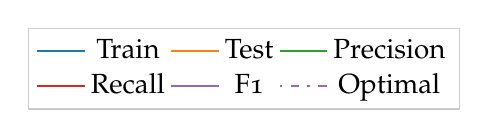
\begin{tikzpicture}

\definecolor{color0}{rgb}{0.12156862745098,0.466666666666667,0.705882352941177}
\definecolor{color1}{rgb}{1,0.498039215686275,0.0549019607843137}
\definecolor{color2}{rgb}{0.172549019607843,0.627450980392157,0.172549019607843}
\definecolor{color3}{rgb}{0.83921568627451,0.152941176470588,0.156862745098039}
\definecolor{color4}{rgb}{0.580392156862745,0.403921568627451,0.741176470588235}
\begin{axis}[%
 hide axis,
 xmin=10,
 xmax=50,
 ymin=0,
 ymax=0.4,
 legend columns=3,
 legend style={
   fill opacity=1,
   draw opacity=1,
   text opacity=1,
   align=center,
   anchor=north,
   draw=white!80!black
 },
 ]
 \addlegendimage{semithick, color0}
 \addlegendentry{Train};
 \addlegendimage{semithick, color1}
 \addlegendentry{Test};
 \addlegendimage{semithick, color2}
 \addlegendentry{Precision};
 \addlegendimage{semithick, color3}
 \addlegendentry{Recall};
 \addlegendimage{semithick, color4}
 \addlegendentry{F1};
 \addlegendimage{semithick, color4, dash pattern=on 1pt off 3pt on 3pt off 3pt}
 \addlegendentry{Optimal};
 \end{axis}

\end{tikzpicture}

  \end{subfigure}
  \par\bigskip
  \begin{subfigure}[b]{0.5\textwidth}
    % This file was created by tikzplotlib v0.9.8.
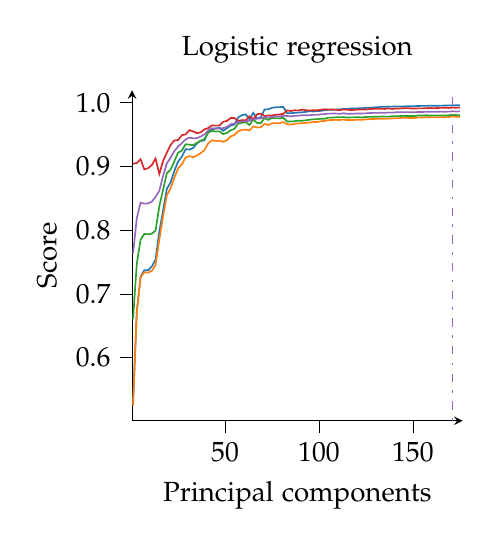
\begin{tikzpicture}

\definecolor{color0}{rgb}{0.12156862745098,0.466666666666667,0.705882352941177}
\definecolor{color1}{rgb}{1,0.498039215686275,0.0549019607843137}
\definecolor{color2}{rgb}{0.172549019607843,0.627450980392157,0.172549019607843}
\definecolor{color3}{rgb}{0.83921568627451,0.152941176470588,0.156862745098039}
\definecolor{color4}{rgb}{0.580392156862745,0.403921568627451,0.741176470588235}

\begin{axis}[
height=2.275590092707901in,
tick align=outside,
tick pos=left,
title={Logistic regression},
width=2.275590092707901in,
x grid style={white!69.0196078431373!black},
xlabel={Principal components},
xmin=0.5, xmax=176.5,
xtick style={color=black},
xtick={0,50,100,150,200},
xticklabels={
  \(\displaystyle {0}\),
  \(\displaystyle {50}\),
  \(\displaystyle {100}\),
  \(\displaystyle {150}\),
  \(\displaystyle {200}\)
},
y grid style={white!69.0196078431373!black},
ylabel={Score},
ymin=0.501096391747291, ymax=1.01973669481458,
ytick style={color=black},
ytick={0.5,0.6,0.7,0.8,0.9,1,1.1},
yticklabels={
  \(\displaystyle {0.5}\),
  \(\displaystyle {0.6}\),
  \(\displaystyle {0.7}\),
  \(\displaystyle {0.8}\),
  \(\displaystyle {0.9}\),
  \(\displaystyle {1.0}\),
  \(\displaystyle {1.1}\)
}
]
\addplot [semithick, color0]
table {%
1 0.527978311919052
3 0.672257518373159
5 0.726936676480703
7 0.737204003963955
9 0.7371536474315
11 0.743129561041308
13 0.753973065365214
15 0.797999916812017
17 0.831220812266941
19 0.864665747038822
21 0.875225642897371
23 0.892940839297993
25 0.907831289942227
27 0.915484280258436
29 0.927154832624676
31 0.926581906722074
33 0.929048501041305
35 0.936214158404711
37 0.940204028671267
39 0.940954212283905
41 0.954348432567421
43 0.9579101829613
45 0.95979102944338
47 0.960507784158689
49 0.95611045233101
51 0.959989942496352
53 0.964312267547714
55 0.965762937077656
57 0.977118861393655
59 0.980625775462163
61 0.981674131523199
63 0.973849068329029
65 0.98417222600597
67 0.975393355577146
69 0.976988296303105
71 0.98932929153175
73 0.989743808970333
75 0.992040327743967
77 0.992880248748514
79 0.993137411653601
81 0.993414113504208
83 0.983692753729346
85 0.983623389884701
87 0.984284121882561
89 0.98452486392549
91 0.985083047934706
93 0.98566681374314
95 0.98664953042687
97 0.986322636640174
99 0.986746837221478
101 0.987259146957983
103 0.988267587421691
105 0.98885404647408
107 0.989065862475352
109 0.989253542413724
111 0.989730781585175
113 0.990150137134204
115 0.990077108383256
117 0.991006827686701
119 0.991019162207793
121 0.991312771079592
123 0.991361059142255
125 0.992209056565552
127 0.991993392467355
129 0.992711089064495
131 0.992935244750097
133 0.993596095870027
135 0.993493678432798
137 0.993889977274
139 0.993922059204236
141 0.994264579115255
143 0.994260783657537
145 0.994219836836825
147 0.994575058305901
149 0.994623827364361
151 0.994689063658078
153 0.99491757821692
155 0.995104843642357
157 0.995059970812512
159 0.995513002930682
161 0.995309109938055
163 0.995398594494915
165 0.99546426365274
167 0.995623313596039
169 0.995868153409378
171 0.995729627261883
173 0.996162135584249
175 0.995978665616529
};
\addplot [semithick, color1]
table {%
1 0.524670950977623
3 0.670867772619925
5 0.725863108394313
7 0.733927442763526
9 0.733555795752711
11 0.736184000561332
13 0.745465701046404
15 0.785273990017892
17 0.821643763767867
19 0.854757534127692
21 0.865826097874878
23 0.882614449866961
25 0.896823087639802
27 0.903405199983751
29 0.914149433405531
31 0.916217593233734
33 0.914707877943531
35 0.917110720886905
37 0.92093593844921
39 0.925600873572896
41 0.936269081594404
43 0.941212773441611
45 0.940024320077405
47 0.940302539473271
49 0.938740125450312
51 0.94121085355698
53 0.947146572274262
55 0.949563968303208
57 0.955407434232757
59 0.957350491811754
61 0.957949057276174
63 0.956670804181923
65 0.962797141730786
67 0.961288712057005
69 0.961339015896405
71 0.966930102166114
73 0.965076521181973
75 0.967955056050106
77 0.967817135951282
79 0.968013692622731
81 0.969581622101708
83 0.966388905661144
85 0.965800496335647
87 0.966843609493896
89 0.967544083948675
91 0.968048265317993
93 0.968286007415491
95 0.968979568623758
97 0.969720057370344
99 0.969798328560165
101 0.97100459313587
103 0.971399663293135
105 0.972718471238199
107 0.972996212393989
109 0.973160320291597
111 0.972949300089185
113 0.973716280843254
115 0.972803655674531
117 0.972867637364768
119 0.973066455059281
121 0.973436930935855
123 0.973276997021617
125 0.973800030559356
127 0.974367715378834
129 0.974564924321739
131 0.974746235013452
133 0.975019149914415
135 0.974825636714805
137 0.975136478915891
139 0.975366177255345
141 0.975933383834747
143 0.97593290559467
145 0.976490474897936
147 0.976224936250044
149 0.97611034651171
151 0.976116303278068
153 0.977110417139829
155 0.976754404794218
157 0.977391375798836
159 0.977141909433516
161 0.977032624190085
163 0.977401491315049
165 0.977503878545485
167 0.977239470409126
169 0.977584888998447
171 0.978416503714208
173 0.977958582378238
175 0.978155313081066
};
\addplot [semithick, color2]
table {%
1 0.660526209531335
3 0.747271763749716
5 0.784917402501545
7 0.794267176756586
9 0.793511475403584
11 0.794620562078218
13 0.799523152230156
15 0.837581215874355
17 0.863697781589945
19 0.889480285672649
21 0.895088519217677
23 0.908204106634087
25 0.921655479971229
27 0.924944626117226
29 0.934982733626013
31 0.934221489453499
33 0.933492384550335
35 0.937090811707038
37 0.940412513912378
39 0.942984820378985
41 0.953053634341826
43 0.955921520338845
45 0.954978817159891
47 0.955164046043096
49 0.950861081645013
51 0.952776616955171
53 0.956619619067437
55 0.959181649945466
57 0.967304721177759
59 0.968682184215419
61 0.969544860690647
63 0.965172494479605
65 0.973618553063717
67 0.968434814374178
69 0.967925791547072
71 0.975634040039191
73 0.973176998920976
75 0.97621418482231
77 0.975489402808498
79 0.9754573020742
81 0.976602372231858
83 0.970652590698134
85 0.970663060426771
87 0.971014489855003
89 0.971919589679479
91 0.971795111996232
93 0.972508187686635
95 0.973404234589117
97 0.97400655763931
99 0.974200947121328
101 0.97495293560689
103 0.974922176310523
105 0.976618141603626
107 0.976796274124154
109 0.977163964798968
111 0.977310022601592
113 0.977527482926915
115 0.976778742617798
117 0.977109804939133
119 0.977138645750667
121 0.977317819037685
123 0.976950737393212
125 0.977715629784876
127 0.977895865047589
129 0.977924905340252
131 0.978112332680922
133 0.978327531824792
135 0.978320150536469
137 0.978162442434481
139 0.97887430522476
141 0.979094557757062
143 0.979083321261843
145 0.979465600334943
147 0.979096858028989
149 0.979273497447592
151 0.979264647632088
153 0.98019568430901
155 0.979852563049805
157 0.980407553452011
159 0.97987666478631
161 0.980033763597739
163 0.980239959065847
165 0.980222596059216
167 0.979858928781099
169 0.980414030151713
171 0.98099643138722
173 0.98060989765861
175 0.980626337513261
};
\addplot [semithick, color3]
table {%
1 0.904293639406982
3 0.905471066475371
5 0.911330463892874
7 0.895509325681492
9 0.89726924916308
11 0.902149210903874
13 0.912498326159732
15 0.888276422764228
17 0.908609277857484
19 0.921690100430416
21 0.933788617886179
23 0.940827355332377
25 0.94160306073649
27 0.949027259684362
29 0.950390243902439
31 0.95703299856528
33 0.955081779053085
35 0.952342419894787
37 0.953516021042563
39 0.958209469153515
41 0.960153993304639
43 0.9646456241033
45 0.964064084170254
47 0.964260162601626
49 0.970118603538976
51 0.971485413677666
53 0.976172166427547
55 0.97597800095648
57 0.971487326637972
59 0.972854136776662
61 0.972268770923003
63 0.978711621233859
65 0.974419894787183
67 0.981837398373984
69 0.983006217120995
71 0.979104734576758
73 0.980082257293161
75 0.980083213773314
77 0.981252032520325
79 0.981645145863223
81 0.982618842659015
83 0.988089909134386
85 0.986916307986609
87 0.988285031085605
89 0.987893830703013
91 0.989262553802009
93 0.988286944045911
95 0.987894787183166
97 0.988285031085605
99 0.988090865614539
101 0.989068388330942
103 0.98984887613582
105 0.989262553802009
107 0.989457675753228
109 0.989068388330942
111 0.988285987565758
113 0.989459588713534
115 0.989069344811095
117 0.988483022477284
119 0.988874222859876
121 0.989264466762315
123 0.989655667144907
125 0.989263510282162
127 0.990044954567193
129 0.990436154949785
131 0.990435198469632
133 0.990630320420851
135 0.990240076518412
137 0.99121568627451
139 0.990240076518412
141 0.99102056432329
143 0.991019607843137
145 0.991410808225729
147 0.991606886657102
149 0.99102056432329
151 0.991019607843137
153 0.99121568627451
155 0.991214729794357
157 0.991410808225729
159 0.991996174079388
161 0.991410808225729
163 0.991801052128168
165 0.991996174079388
167 0.992191296030607
169 0.991801052128168
171 0.992386417981827
173 0.992191296030608
175 0.992581539933046
};
\addplot [semithick, color4]
table {%
1 0.76327826913597
3 0.818651569656171
5 0.843331146676396
7 0.84169792475628
9 0.842067908612409
11 0.844813503673515
13 0.852124363378905
15 0.861976720922363
17 0.885282648968169
19 0.90496551535333
21 0.913808723923361
23 0.924073146040379
25 0.931375978080348
27 0.936731426464567
29 0.942533198420864
31 0.945370642159646
33 0.944072143424975
35 0.944579525921237
37 0.946839897656345
39 0.950460462558033
41 0.956470634227884
43 0.960164381825251
45 0.959398895015101
47 0.959577982179569
49 0.960312496475416
51 0.961950228479052
53 0.966214111548991
55 0.967423688855172
57 0.969320345634248
59 0.970697341062533
61 0.970854625027329
63 0.971833175254563
65 0.973959307480675
67 0.975027042687256
69 0.975346597911891
71 0.977319633868194
73 0.97657707431891
75 0.978095920537375
77 0.978319877721788
79 0.978511612913037
81 0.979567956211785
83 0.979238141098257
85 0.978651945000747
87 0.979519430282232
89 0.979793635143959
91 0.980395644616177
93 0.9802832228004
95 0.980553741070374
97 0.981048727805319
99 0.981042530303693
101 0.981911935989541
103 0.98229786639816
105 0.982860073758902
107 0.983051506088867
109 0.983041644918783
111 0.982736151995381
113 0.983428784105583
115 0.982852244274254
117 0.982737730874411
119 0.982936953339814
121 0.983228597277582
123 0.983234206366182
125 0.983421162390887
127 0.98390753416485
129 0.984105263945853
131 0.984201711076164
133 0.984398525513513
135 0.984201523780763
137 0.984602971088457
139 0.984486514671602
141 0.984981991879854
143 0.984983090467204
145 0.985365284099043
147 0.985277860703882
149 0.98507709601412
151 0.985075740767988
153 0.985643232324871
155 0.985463068376293
157 0.985842563116465
159 0.98585600923236
161 0.985655424765855
163 0.985952037646302
165 0.986039552285513
167 0.985952994477143
169 0.986040974394843
171 0.986623508036311
173 0.986333887205196
175 0.986530816878293
};
\addplot [semithick, color4, dash pattern=on 1pt off 3pt on 3pt off 3pt]
table {%
171 0.501096391747291
171 1.01973669481458
};
\end{axis}

\end{tikzpicture}

    \caption{}
    \label{fig:q1-LOG}
  \end{subfigure}%
    \hfill
  \begin{subfigure}[b]{0.5\textwidth}
    % This file was created by tikzplotlib v0.9.8.
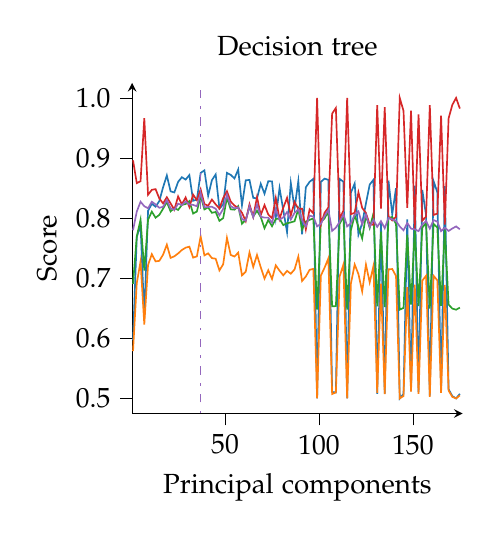
\begin{tikzpicture}

\definecolor{color0}{rgb}{0.12156862745098,0.466666666666667,0.705882352941177}
\definecolor{color1}{rgb}{1,0.498039215686275,0.0549019607843137}
\definecolor{color2}{rgb}{0.172549019607843,0.627450980392157,0.172549019607843}
\definecolor{color3}{rgb}{0.83921568627451,0.152941176470588,0.156862745098039}
\definecolor{color4}{rgb}{0.580392156862745,0.403921568627451,0.741176470588235}

\begin{axis}[
height=2.275590092707901in,
tick align=outside,
tick pos=left,
title={Decision tree},
width=2.275590092707901in,
x grid style={white!69.0196078431373!black},
xlabel={Principal components},
xmin=0.5, xmax=176.5,
xtick style={color=black},
xtick={0,50,100,150,200},
xticklabels={
  \(\displaystyle {0}\),
  \(\displaystyle {50}\),
  \(\displaystyle {100}\),
  \(\displaystyle {150}\),
  \(\displaystyle {200}\)
},
y grid style={white!69.0196078431373!black},
ylabel={Score},
ymin=0.475, ymax=1.025,
ytick style={color=black},
ytick={0.4,0.5,0.6,0.7,0.8,0.9,1,1.1},
yticklabels={
  \(\displaystyle {0.4}\),
  \(\displaystyle {0.5}\),
  \(\displaystyle {0.6}\),
  \(\displaystyle {0.7}\),
  \(\displaystyle {0.8}\),
  \(\displaystyle {0.9}\),
  \(\displaystyle {1.0}\),
  \(\displaystyle {1.1}\)
}
]
\addplot [semithick, color0]
table {%
1 0.596497717449444
3 0.768506780224986
5 0.789072473394637
7 0.635431052744238
9 0.812246594635627
11 0.823822913593586
13 0.819063114844103
15 0.828455297352151
17 0.851312841778874
19 0.871054460654502
21 0.844573082460765
23 0.842712085180569
25 0.860318528354227
27 0.868077782369472
29 0.864111971448012
31 0.871685010557694
33 0.828865734907841
35 0.830932878731714
37 0.875222132631586
39 0.879464758724772
41 0.837337279686309
43 0.863188141109501
45 0.872661827996532
47 0.815872474339355
49 0.822693179431544
51 0.875248923103878
53 0.87197968309829
55 0.865976578541978
57 0.880933944970876
59 0.821406402368332
61 0.862939330364918
63 0.863531425331119
65 0.833696454122586
67 0.83298007274486
69 0.857111340325214
71 0.840624043555583
73 0.861380554172503
75 0.861108374817675
77 0.800606474192092
79 0.850138667208445
81 0.813133334410096
83 0.776733277842867
85 0.858524949760363
87 0.816409811034941
89 0.861656021029682
91 0.772931198434995
93 0.851300184110581
95 0.860396061377324
97 0.865314146220163
99 0.5
101 0.860272513457213
103 0.865730323533595
105 0.863562280432173
107 0.510780648950084
109 0.510025077065436
111 0.865172729428312
113 0.860575017255092
115 0.5
117 0.842407371293759
119 0.85746071020843
121 0.772354167423015
123 0.791509904415402
125 0.824349545979451
127 0.855896205345502
129 0.863750622916912
131 0.507692855226488
133 0.794366735038516
135 0.507977055241831
137 0.86246681579223
139 0.80625641462588
141 0.849912698261898
143 0.5
145 0.507400252960791
147 0.797810076370395
149 0.512379354442437
151 0.854027328023614
153 0.510660948072043
155 0.846926636549466
157 0.805216696040322
159 0.504692860701829
161 0.861615559155597
163 0.843237281200769
165 0.51268667018346
167 0.853159400642768
169 0.515295944317397
171 0.503806676631789
173 0.5
175 0.507660067968993
};
\addplot [semithick, color1]
table {%
1 0.578768326842932
3 0.691790567314599
5 0.727748869488468
7 0.623064681508728
9 0.721959461305946
11 0.740025114989964
13 0.728012304526293
15 0.728950643408319
17 0.739168797050791
19 0.755813493294483
21 0.733819262180812
23 0.736502631243664
25 0.74123106381643
27 0.746944824666848
29 0.750800204129114
31 0.752515759303062
33 0.734273446227535
35 0.736303831552397
37 0.769742552657187
39 0.738027412942765
41 0.741400498828404
43 0.73342747646191
45 0.732457103803948
47 0.712984303015867
49 0.723216204214052
51 0.767099409308878
53 0.738716267917846
55 0.736103655305234
57 0.742504820715366
59 0.704777293844367
61 0.710847611292375
63 0.742733149884872
65 0.718701609120906
67 0.738685802732431
69 0.718188129767398
71 0.69930786751088
73 0.713248353395412
75 0.698764008833593
77 0.721435647627542
79 0.712593752135
81 0.704805617566737
83 0.712219320622118
85 0.707513599836771
87 0.714646026637418
89 0.736076347150594
91 0.695413534563463
93 0.702911964588077
95 0.713967476905067
97 0.715624707562656
99 0.5
101 0.704367860789669
103 0.717735700344739
105 0.733097151978788
107 0.507334628643811
109 0.509988134475939
111 0.702994975247845
113 0.722606732937077
115 0.5
117 0.69098720892444
119 0.722855625045008
121 0.70701382280005
123 0.677964524834324
125 0.72265892988705
127 0.693069657328983
129 0.720387790383128
131 0.50918391562294
133 0.690996190236147
135 0.507213854098
137 0.714920114980732
139 0.715284894445583
141 0.703893530187289
143 0.5
145 0.504043067457702
147 0.685176994067238
149 0.511407359450042
151 0.689459213415096
153 0.507687988511159
155 0.696004412180165
157 0.704069485605712
159 0.502599868160844
161 0.704102806382936
163 0.696546110006297
165 0.509182134686439
167 0.6889112523058
169 0.51316191934915
171 0.502532190727313
173 0.5
175 0.505121743489749
};
\addplot [semithick, color2]
table {%
1 0.690646028080078
3 0.76977795012896
5 0.797266579935977
7 0.712665710384953
9 0.797395011924239
11 0.810835730414563
13 0.800721666817829
15 0.805359862993895
17 0.815671846991249
19 0.826815874616206
21 0.811172521251474
23 0.816976708496276
25 0.81355840819195
27 0.822062539826173
29 0.823422923735299
31 0.828356808638562
33 0.807611589533691
35 0.811008393709643
37 0.836904435636554
39 0.814477964339968
41 0.817791500401826
43 0.808810170628359
45 0.810276907853969
47 0.795481007683356
49 0.800014895188039
51 0.833907288587748
53 0.814636312882636
55 0.8140703790893
57 0.820045019066581
59 0.790604112329787
61 0.797295667094074
63 0.81881134153839
65 0.802738911050435
67 0.812316041527201
69 0.801834690970316
71 0.783252195964148
73 0.796868551574173
75 0.786516502608262
77 0.798731034138699
79 0.798962968289488
81 0.788423442064658
83 0.791442017252198
85 0.792905154664528
87 0.794769766926958
89 0.814926677788018
91 0.7812266796863
93 0.794165600658011
95 0.79717622519109
97 0.799454716161802
99 0.647691969811924
101 0.793185246483871
103 0.799651045331469
105 0.811755230940412
107 0.653249710619967
109 0.653576827149121
111 0.79003483898687
113 0.80343891381361
115 0.647691969811924
117 0.77975373251055
119 0.804913195581554
121 0.785309784717675
123 0.766122974132401
125 0.804872282827964
127 0.783694457722852
129 0.80752545515596
131 0.653152567864102
133 0.777494620076289
135 0.652107381621955
137 0.80007840746219
139 0.802023435566857
141 0.790203831225899
143 0.647691969811924
145 0.650558738663497
147 0.772575263592028
149 0.656266076861863
151 0.782563328714032
153 0.653630757156716
155 0.78415133429832
157 0.791886530924938
159 0.649509593014578
161 0.79044713997428
163 0.784492867064612
165 0.654206818351503
167 0.781295695131415
169 0.656166518971361
171 0.649420327841799
173 0.647691969811924
175 0.651030218400474
};
\addplot [semithick, color3]
table {%
1 0.896108082257293
3 0.85820468675275
5 0.861334289813486
7 0.96641893830703
9 0.838841702534672
11 0.847083692013391
13 0.848228598756576
15 0.832624581539933
17 0.824447632711621
19 0.834783357245337
21 0.8244725011956
23 0.814092778574845
25 0.836130081300813
27 0.822876135820182
29 0.834383548541368
31 0.81838737446198
33 0.839061692969871
35 0.829908177905309
37 0.847869918699187
39 0.823249163079866
41 0.820719273075084
43 0.830870396939264
45 0.822864658058345
47 0.816020086083214
49 0.833195600191296
51 0.844739359158298
53 0.827567670970827
55 0.820901004304161
57 0.816808225729316
59 0.808959349593496
61 0.795131516021043
63 0.823043519846963
65 0.802168340506935
67 0.834984218077475
69 0.805073170731707
71 0.821659493065519
73 0.806078431372549
75 0.799786704925873
77 0.833614538498326
79 0.798639885222382
81 0.817378287900526
83 0.833779053084649
85 0.804682926829268
87 0.826782400765184
89 0.815418460066954
91 0.815595408895265
93 0.781271162123386
95 0.814672405547585
97 0.808028694404591
99 1
101 0.789662362505978
103 0.808978479196557
105 0.817758010521282
107 0.973787661406026
109 0.983219512195122
111 0.79885031085605
113 0.812475370636059
115 1
117 0.806649450023912
119 0.808787183165949
121 0.842985174557628
123 0.817000478240077
125 0.808599713055954
127 0.789263510282162
129 0.789034911525586
131 0.98809756097561
133 0.816023912003826
135 0.984585365853659
137 0.802546150167384
139 0.796284074605452
141 0.802133907221425
143 1
145 0.978536585365854
147 0.816975609756098
149 0.978731707317073
151 0.781843137254902
153 0.972682926829268
155 0.79591487326638
157 0.802318507890961
159 0.98790243902439
161 0.805261597321856
163 0.80745193687231
165 0.970275466284074
167 0.789251076040172
169 0.965982783357245
171 0.988487804878049
173 1
175 0.982219033955045
};
\addplot [semithick, color4]
table {%
1 0.779835815655286
3 0.810860357787374
5 0.827212136873701
7 0.819854736749766
9 0.816362260142288
11 0.827301018796805
13 0.822822811449125
15 0.817161204645316
17 0.818798213116716
19 0.830143105303606
21 0.816410276017348
23 0.813713650026485
25 0.824109298073981
27 0.821822540679694
29 0.827699790006685
31 0.822652858207086
33 0.822008073434729
35 0.81974863919911
37 0.841067190862751
39 0.817987020508943
41 0.818622639639426
43 0.818890811753971
45 0.81559144725181
47 0.804581546338155
49 0.815380439624153
51 0.838892195269103
53 0.819884850253967
55 0.816329074489787
57 0.81783619879634
59 0.798561424747511
61 0.795564081309575
63 0.819974877318493
65 0.801543267470842
67 0.822747956329741
69 0.802453099769105
71 0.800780858809059
73 0.800860868596634
75 0.792196807552761
77 0.814402840887597
79 0.797347626490337
81 0.801355119305887
83 0.810126352140618
85 0.797672935774432
87 0.808814427555639
89 0.81448538251746
91 0.796528005130148
93 0.786050925371033
95 0.804089631659403
97 0.802547088574708
99 0.786180105478537
101 0.790386746819531
103 0.803759748113057
105 0.813563395829392
107 0.778803831451768
109 0.784111976229354
111 0.793827236837649
113 0.806789155165574
115 0.786180105478537
117 0.791522831527967
119 0.805896578797655
121 0.81136306750649
123 0.789623694041504
125 0.805948662646561
127 0.785504771631667
129 0.797273553824855
131 0.785464380280141
133 0.794953667440545
135 0.783180172990284
137 0.800354455798982
139 0.797828453841038
141 0.795158049075743
143 0.786180105478537
145 0.779706743696419
147 0.791838104123069
149 0.78253084708925
151 0.781375124784412
153 0.778386953300618
155 0.789189726192279
157 0.795330246560796
159 0.782536728293543
161 0.796770567228836
163 0.794160716848915
165 0.778298989274557
167 0.784061079384507
169 0.778675881534646
171 0.78277910149212
173 0.786180105478537
175 0.78146768573516
};
\addplot [semithick, color4, dash pattern=on 1pt off 3pt on 3pt off 3pt]
table {%
37 0.475
37 1.025
};
\end{axis}

\end{tikzpicture}

    \caption{}
    \label{fig:q1-DT}
  \end{subfigure}
  \begin{subfigure}[b]{0.5\textwidth}
    % This file was created by tikzplotlib v0.9.8.
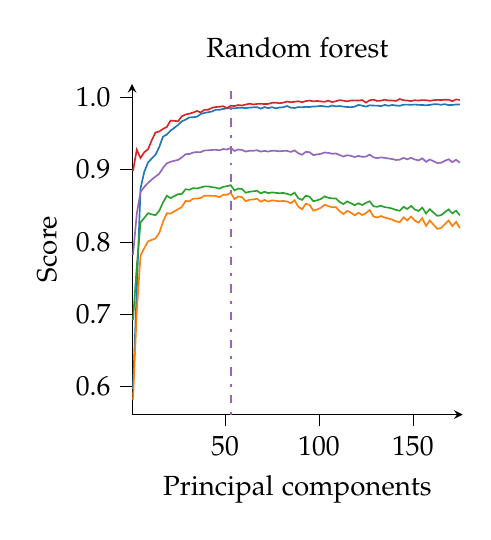
\begin{tikzpicture}

\definecolor{color0}{rgb}{0.12156862745098,0.466666666666667,0.705882352941177}
\definecolor{color1}{rgb}{1,0.498039215686275,0.0549019607843137}
\definecolor{color2}{rgb}{0.172549019607843,0.627450980392157,0.172549019607843}
\definecolor{color3}{rgb}{0.83921568627451,0.152941176470588,0.156862745098039}
\definecolor{color4}{rgb}{0.580392156862745,0.403921568627451,0.741176470588235}

\begin{axis}[
height=2.275590092707901in,
tick align=outside,
tick pos=left,
title={Random forest},
width=2.275590092707901in,
x grid style={white!69.0196078431373!black},
xlabel={Principal components},
xmin=0.5, xmax=176.5,
xtick style={color=black},
xtick={0,50,100,150,200},
xticklabels={
  \(\displaystyle {0}\),
  \(\displaystyle {50}\),
  \(\displaystyle {100}\),
  \(\displaystyle {150}\),
  \(\displaystyle {200}\)
},
y grid style={white!69.0196078431373!black},
ylabel={Score},
ymin=0.561477496219318, ymax=1.01863347578979,
ytick style={color=black},
ytick={0.5,0.6,0.7,0.8,0.9,1,1.1},
yticklabels={
  \(\displaystyle {0.5}\),
  \(\displaystyle {0.6}\),
  \(\displaystyle {0.7}\),
  \(\displaystyle {0.8}\),
  \(\displaystyle {0.9}\),
  \(\displaystyle {1.0}\),
  \(\displaystyle {1.1}\)
}
]
\addplot [semithick, color0]
table {%
1 0.59722126125097
3 0.734835181637817
5 0.874130828532667
7 0.897255518443422
9 0.910021818468807
11 0.915599575494005
13 0.920733589922345
15 0.9317329485511
17 0.94588067007524
19 0.948656264308016
21 0.954161909191095
23 0.957986929412309
25 0.962013094984398
27 0.966959458360583
29 0.969353278765588
31 0.972295923206796
33 0.97267159231806
35 0.973207693492041
37 0.977008734669172
39 0.97854605353126
41 0.979517697583872
43 0.980570103939348
45 0.982802055768921
47 0.982847704985427
49 0.984108576177909
51 0.984938801507521
53 0.985307317730692
55 0.984796479902308
57 0.985800164675294
59 0.985817527419282
61 0.985150498386723
63 0.985909698953989
65 0.986274224443756
67 0.986538408582648
69 0.984499040629036
71 0.986611235791801
73 0.985339245595103
75 0.986502003825798
77 0.984878208048563
79 0.986051587695095
81 0.986408148966353
83 0.988097139827444
85 0.985804161674806
87 0.985441912705817
89 0.986660549914611
91 0.986482487738967
93 0.986882007193021
95 0.986823869389597
97 0.987423889462149
99 0.987607258658971
101 0.988276340263476
103 0.987496515129508
105 0.987113350710469
107 0.988770218431461
109 0.987631648902874
111 0.988077422198818
113 0.987341059102131
115 0.986733981749148
117 0.986533380359752
119 0.987206529954149
121 0.989650996915168
123 0.988594511140455
125 0.987270045769131
127 0.989113484948624
129 0.988729947226513
131 0.98862031217692
133 0.987940545539679
135 0.989623848703039
137 0.988460788159652
139 0.989561008503821
141 0.988799482832435
143 0.988419811558422
145 0.989945382173628
147 0.990035773668564
149 0.989875111390907
151 0.990120988693737
153 0.989721267697889
155 0.989516497547703
157 0.989201760254715
159 0.989627916692931
161 0.990549096933001
163 0.990548794620309
165 0.989875615245394
167 0.990708419408475
169 0.989361918677886
171 0.989630876202953
173 0.990188710423507
175 0.990348969617574
};
\addplot [semithick, color1]
table {%
1 0.582257313472522
3 0.703576908020954
5 0.781639726424518
7 0.791747155948734
9 0.800985273344671
11 0.803008499378657
13 0.805048287937456
15 0.812919290986005
17 0.82813933496932
19 0.839933116555785
21 0.839309142048382
23 0.842509138263084
25 0.845439741288737
27 0.848610054766798
29 0.85678946496199
31 0.856277009947024
33 0.859955337639341
35 0.860123259455397
37 0.860938364271219
39 0.863959723045448
41 0.864232333737714
43 0.863886222254228
45 0.863757780633677
47 0.86197592088912
49 0.865409748803938
51 0.865321722162827
53 0.868231867499802
55 0.859592104145547
57 0.86297595089453
59 0.862128074631303
61 0.856429656701178
63 0.858556111963573
65 0.858861994501162
67 0.859977785379148
69 0.855774022793033
71 0.858280168824287
73 0.856032169954336
75 0.857700992855943
77 0.857078007142211
79 0.856340272892281
81 0.856909088223292
83 0.856077432884822
85 0.853622298820649
87 0.857868162690257
89 0.848907689971176
91 0.845332401780752
93 0.852978389180326
95 0.85137425932799
97 0.843434507421954
99 0.845169414238998
101 0.847376905343548
103 0.851579552651647
105 0.849655554970835
107 0.848125752212553
109 0.848365062438951
111 0.842686412534691
113 0.838695782531866
115 0.843074147061593
117 0.840605276059006
119 0.836932097295082
121 0.840583884048016
123 0.837312703921384
125 0.840018805083009
127 0.844207255677485
129 0.83544900742103
131 0.833865847195833
133 0.836018819854903
135 0.833836560068985
137 0.832537864981194
139 0.831074075048609
141 0.828459007070198
143 0.82766717675864
145 0.834147079596506
147 0.830003602957333
149 0.83537769010043
151 0.829650792881424
153 0.826785447468374
155 0.83298837959706
157 0.822308450539082
159 0.829821525050363
161 0.823918158627986
163 0.818280026644804
165 0.819538563876441
167 0.824830290323117
169 0.829722329933951
171 0.822160585724072
173 0.827917295395416
175 0.819251633217559
};
\addplot [semithick, color2]
table {%
1 0.692467628538399
3 0.766586579272089
5 0.82724677813506
7 0.833419252740925
9 0.839880037128331
11 0.838178996076448
13 0.837216511296203
15 0.843361051374326
17 0.854912213512556
19 0.864066067904858
21 0.860791910450187
23 0.863559885719853
25 0.866150919723699
27 0.866638036819272
29 0.872951999889314
31 0.872298423253009
33 0.874606549787485
35 0.87414080057987
37 0.875385333746744
39 0.876877302194397
41 0.877004526400047
43 0.875881832997461
45 0.875249715545295
47 0.873762509241852
49 0.876387752799132
51 0.877239605645773
53 0.878699686918563
55 0.871448023788113
57 0.874024029005874
59 0.873254174985233
61 0.868305261931905
63 0.869520154629273
65 0.87010253722489
67 0.870959811344763
69 0.867431710746304
71 0.869549539380749
73 0.8676637127434
75 0.868593988059667
77 0.868018836741884
79 0.867541987853898
81 0.867897136839601
83 0.866736389213694
85 0.865044755497167
87 0.868266837595929
89 0.860656485035825
91 0.85826774185107
93 0.864111532940603
95 0.862574607759479
97 0.85645265492087
99 0.857756215209664
101 0.859559874014496
103 0.863124954158872
105 0.861198961396998
107 0.860384406268404
109 0.860250743224491
111 0.855405719700441
113 0.852450048249788
115 0.856210690732954
117 0.853756517918072
119 0.85092815014534
121 0.853629080319015
123 0.851107090716629
125 0.854183268387832
127 0.856424770547738
129 0.849550808090464
131 0.848749447038843
133 0.850227306881538
135 0.848201146373335
137 0.847570784823426
139 0.846266670716523
141 0.844449561537903
143 0.84322225694787
145 0.848684919786359
147 0.845706920310201
149 0.849950255477111
151 0.845009534669244
153 0.842963522910178
155 0.847607984438977
157 0.839378965326265
159 0.845470319646793
161 0.840701996211717
163 0.836252514189232
165 0.8371611474015
167 0.841203939044478
169 0.845062320986516
171 0.839640601411967
173 0.843389740830659
175 0.836905417068356
};
\addplot [semithick, color3]
table {%
1 0.898439980870397
3 0.927752271640363
5 0.91622668579627
7 0.924234337637494
9 0.928334768053563
11 0.941023433763749
13 0.951573409851746
15 0.952936394069823
17 0.956452415112386
19 0.959184122429459
21 0.96797800095648
23 0.967585844093735
25 0.967002391200382
27 0.97403156384505
29 0.97637494021999
31 0.977547584887614
33 0.979109516977523
35 0.98125681492109
37 0.979302725968436
39 0.982819703491153
41 0.98301099952176
43 0.985552367288379
45 0.986724055475849
47 0.987111429937829
49 0.987894787183166
51 0.985164036346246
53 0.988481109516978
55 0.988087039693926
57 0.989455762792922
59 0.988873266379723
61 0.99004399808704
63 0.991410808225729
65 0.990240076518412
67 0.99102056432329
69 0.991216642754663
71 0.990823529411765
73 0.991018651362984
75 0.992583452893352
77 0.992775705404113
79 0.991995217599235
81 0.992775705404113
83 0.994339550454328
85 0.993361071257772
87 0.993947393591583
89 0.994729794356767
91 0.993361071257772
93 0.994923959827834
95 0.995705404112865
97 0.994529890004782
99 0.995120038259206
101 0.994531802965088
103 0.993947393591583
105 0.995511238641798
107 0.993555236728838
109 0.994728837876614
111 0.99628981348637
113 0.995509325681492
115 0.994529890004783
117 0.995705404112865
119 0.995897656623625
121 0.995704447632712
123 0.996288857006217
125 0.992775705404113
127 0.996094691535151
129 0.996876135820182
131 0.995119081779053
133 0.995509325681492
135 0.996875179340029
137 0.995706360593018
139 0.995703491152559
141 0.995116212338594
143 0.997853658536585
145 0.996096604495457
147 0.995705404112865
149 0.994922046867528
151 0.996093735054998
153 0.995707317073171
155 0.996288857006217
157 0.996093735054998
159 0.995312290769967
161 0.996095648015304
163 0.996679100908656
165 0.996290769966523
167 0.996874222859876
169 0.996877092300335
171 0.994729794356767
173 0.997266379722621
175 0.996485891917743
};
\addplot [semithick, color4]
table {%
1 0.782025546315744
3 0.839332247617965
5 0.869291935346631
7 0.876287400220564
9 0.881719876917005
11 0.886501926773996
13 0.890577135428357
15 0.894586157109603
17 0.902626078302082
19 0.908867412969607
21 0.911002534404812
23 0.912394537250977
25 0.913612386603002
27 0.917040810214638
29 0.921586353886293
31 0.921705495448873
33 0.923772637002286
35 0.924449559173957
37 0.924289330167027
39 0.926683900222187
41 0.926844121101328
43 0.927359835976764
45 0.927568469597156
47 0.926875116709293
49 0.928703109996736
51 0.927933185821485
53 0.930214957378713
55 0.926006778155564
57 0.928012997548613
59 0.927376114883806
61 0.92505556803743
63 0.926382421098627
65 0.926204578071884
67 0.926989985329128
69 0.925068082063457
71 0.926112556533024
73 0.925128308662709
75 0.926344151086026
77 0.926095765530172
79 0.925497361846843
81 0.92602164468961
83 0.926029111458864
85 0.924638849009363
87 0.926747444962935
89 0.922747050628139
91 0.920766326401275
93 0.924751337037949
95 0.924223368507371
97 0.920207031657441
99 0.921186911768155
101 0.922017175008161
103 0.923808885050341
105 0.923354696176
107 0.922086887457966
109 0.922505484193032
111 0.920345544368648
113 0.918296695412141
115 0.920054066064396
117 0.919172401537812
119 0.917575764396796
121 0.919145554126255
123 0.917847932366789
125 0.918159729815988
127 0.920913893838103
129 0.917180350349977
131 0.915962953034149
133 0.91702598913301
135 0.916408115220916
137 0.91552476265976
139 0.914818228398054
141 0.913480200908371
143 0.913886301691896
145 0.916357916108921
147 0.91441617452562
149 0.916602373470742
151 0.914255102082737
153 0.912864332511622
155 0.915842851809721
157 0.910929272358059
159 0.914153585265048
161 0.911684877045454
163 0.90930579712454
165 0.90971518910248
167 0.91232063655394
169 0.914544531236055
171 0.910499991285467
173 0.913785507062653
175 0.909653264887392
};
\addplot [semithick, color4, dash pattern=on 1pt off 3pt on 3pt off 3pt]
table {%
53 0.561477496219318
53 1.01863347578979
};
\end{axis}

\end{tikzpicture}

    \caption{}
    \label{fig:q1-RF}
  \end{subfigure}%
   \hfill
  \begin{subfigure}[b]{0.5\textwidth}
    % This file was created by tikzplotlib v0.9.8.
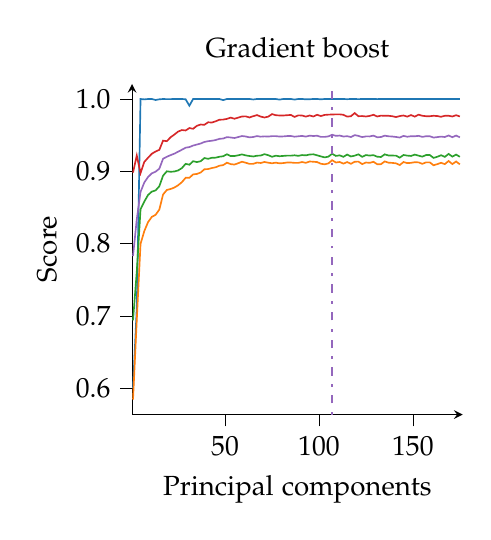
\begin{tikzpicture}

\definecolor{color0}{rgb}{0.12156862745098,0.466666666666667,0.705882352941177}
\definecolor{color1}{rgb}{1,0.498039215686275,0.0549019607843137}
\definecolor{color2}{rgb}{0.172549019607843,0.627450980392157,0.172549019607843}
\definecolor{color3}{rgb}{0.83921568627451,0.152941176470588,0.156862745098039}
\definecolor{color4}{rgb}{0.580392156862745,0.403921568627451,0.741176470588235}

\begin{axis}[
height=2.275590092707901in,
tick align=outside,
tick pos=left,
title={Gradient boost},
width=2.275590092707901in,
x grid style={white!69.0196078431373!black},
xlabel={Principal components},
xmin=0.5, xmax=176.5,
xtick style={color=black},
xtick={0,50,100,150,200},
xticklabels={
  \(\displaystyle {0}\),
  \(\displaystyle {50}\),
  \(\displaystyle {100}\),
  \(\displaystyle {150}\),
  \(\displaystyle {200}\)
},
y grid style={white!69.0196078431373!black},
ylabel={Score},
ymin=0.563723319050758, ymax=1.0207750800452,
ytick style={color=black},
ytick={0.5,0.6,0.7,0.8,0.9,1,1.1},
yticklabels={
  \(\displaystyle {0.5}\),
  \(\displaystyle {0.6}\),
  \(\displaystyle {0.7}\),
  \(\displaystyle {0.8}\),
  \(\displaystyle {0.9}\),
  \(\displaystyle {1.0}\),
  \(\displaystyle {1.1}\)
}
]
\addplot [semithick, color0]
table {%
1 0.600477159352101
3 0.711110568369543
5 0.999955056179775
7 0.999436657216473
9 0.999955156950673
11 0.99997557997558
13 0.99859295910538
15 0.999547270194522
17 0.999955156950673
19 0.999751163187149
21 0.999820627802691
23 0.999930736926253
25 1
27 1
29 0.99955106565224
31 0.990702463238936
33 0.999955156950673
35 0.999910213130448
37 1
39 1
41 1
43 1
45 1
47 0.99997557997558
49 0.998400695237564
51 1
53 1
55 1
57 1
59 1
61 1
63 1
65 0.999302027297593
67 1
69 1
71 0.999955056179775
73 1
75 1
77 0.999955156950673
79 0.999118587110392
81 1
83 1
85 1
87 0.999180460810498
89 1
91 1
93 0.999522779179722
95 0.999612435497859
97 1
99 1
101 0.999506021061118
103 0.999955156950673
105 1
107 1
109 1
111 1
113 1
115 0.999685796342016
117 1
119 1
121 0.999730639391344
123 1
125 1
127 1
129 1
131 0.999820627802691
133 1
135 0.999885793106028
137 1
139 0.999840950056701
141 1
143 1
145 1
147 1
149 1
151 0.999885893876925
153 1
155 1
157 1
159 1
161 1
163 1
165 0.999930636155355
167 1
169 1
171 1
173 1
175 1
};
\addplot [semithick, color1]
table {%
1 0.58449839909596
3 0.694545214460207
5 0.799704305914851
7 0.817293705880506
9 0.829745083267321
11 0.836988816752805
13 0.839783400637776
15 0.847081040919993
17 0.867955878659968
19 0.87421590969941
21 0.875514523541783
23 0.877555405682378
25 0.880676745253144
27 0.884983984958519
29 0.890982781510758
31 0.891022261706265
33 0.895745377320341
35 0.896358977341761
37 0.898318063349268
39 0.902797191124307
41 0.903117281916062
43 0.904540738114626
45 0.905586575302501
47 0.907738566092224
49 0.908567282746981
51 0.91192849202964
53 0.909919309912495
55 0.909325437294232
57 0.911186353908735
59 0.913224885471657
61 0.911877483293911
63 0.910213921033146
65 0.910360161863031
67 0.91205585530191
69 0.91150378991412
71 0.912902971274205
73 0.911880237790568
75 0.911111377774577
77 0.911948511639329
79 0.911031190393099
81 0.911395116319435
83 0.912138822569239
85 0.912144894279399
87 0.91167355036939
89 0.911657552407911
91 0.912826427011147
93 0.911680752591083
95 0.913541495174207
97 0.91322749455748
99 0.912787343810299
101 0.910457244598565
103 0.909633633018138
105 0.910902922803927
107 0.915318068888729
109 0.91217029962941
111 0.912890846318752
113 0.910626007950972
115 0.912759746680478
117 0.910370640675519
119 0.913238963548504
121 0.913389789205069
123 0.909929878279591
125 0.912156848434825
127 0.911657930937701
129 0.913138703932463
131 0.90980067959946
133 0.909867679372342
135 0.9137020813599
137 0.911931498110121
139 0.911617423172301
141 0.911033361861554
143 0.908660443082968
145 0.912837036000953
147 0.911325696725625
149 0.911690842718102
151 0.912595479985006
153 0.912347581748586
155 0.910307789496814
157 0.912343926628001
159 0.912347318162598
161 0.908332720761343
163 0.909919443321165
165 0.911761589012665
167 0.909944211633236
169 0.914256144184767
171 0.910004817022392
173 0.913569959229572
175 0.909633499609468
};
\addplot [semithick, color2]
table {%
1 0.693860588186648
3 0.761266907042525
5 0.847455095699409
7 0.85814946521674
9 0.867229193164921
11 0.871921851038143
13 0.87356458037904
15 0.879345480751021
17 0.893994513647079
19 0.899994454851895
21 0.899328703878698
23 0.899769718339221
25 0.901187798173528
27 0.904422880313242
29 0.910321387822326
31 0.909102861779526
33 0.913910478201278
35 0.912801457246958
37 0.913906080084742
39 0.91831076901138
41 0.917270990829357
43 0.918717072704449
45 0.918862153030851
47 0.920150359004712
49 0.920826270156352
51 0.923535568481933
53 0.921094120415459
55 0.921094507594081
57 0.922126932361603
59 0.923366723230051
61 0.921984531049316
63 0.921162261639504
65 0.920528825005478
67 0.921511506795139
69 0.921843162444666
71 0.923695402292872
73 0.922270995983839
75 0.92008912795755
77 0.92155024870831
79 0.920874046601856
81 0.921262338687648
83 0.921715185188628
85 0.921615133321455
87 0.922134809238973
89 0.92134077392626
91 0.92246364832241
93 0.922053878068597
95 0.923167974403954
97 0.923518774036849
99 0.922111809296067
101 0.92061188203032
103 0.919228917709697
105 0.920279805673989
107 0.924237835907056
109 0.921270649184521
111 0.922065650645469
113 0.920006191574565
115 0.923159988871448
117 0.920544326508925
119 0.921627575969626
121 0.923464786780374
123 0.920025421906584
125 0.922433889259609
127 0.921731268679298
129 0.92238658052776
131 0.920172596238642
133 0.919786576046323
135 0.923474404940506
137 0.921846027100073
139 0.921759437658457
141 0.921703291886696
143 0.918885209818666
145 0.922561460131922
147 0.921714156462307
149 0.921222809281307
151 0.923095589857119
153 0.921659872996399
155 0.920271658901523
157 0.922468143997433
159 0.922483932059776
161 0.918517504107247
163 0.920081759419155
165 0.922239589931981
167 0.919959655128522
169 0.924036637118789
171 0.920339401735935
173 0.923106757820066
175 0.920049529657888
};
\addplot [semithick, color3]
table {%
1 0.898243902439024
3 0.92189287422286
5 0.897474892395983
7 0.912888570062171
9 0.918756575801052
11 0.924228598756576
13 0.927346724055476
15 0.929692969870875
17 0.942395026303204
19 0.941610712577714
21 0.947077953132472
23 0.950792922046867
25 0.954889526542324
27 0.957036824485892
29 0.956457197513152
31 0.959776183644189
33 0.958797704447633
35 0.962898134863701
37 0.964663797226207
39 0.964268770923003
41 0.967788617886179
43 0.967395504543281
45 0.969152558584409
47 0.97130081300813
49 0.971500717360115
51 0.972473457675753
53 0.974230511716882
55 0.972669536107126
57 0.974232424677188
59 0.975793400286944
61 0.975984696317551
63 0.974430416068866
65 0.976183644189383
67 0.977747489239598
69 0.975594452415112
71 0.974425633668101
73 0.975594452415112
75 0.979111429937829
77 0.977545671927308
79 0.97716212338594
81 0.977156384505022
83 0.977546628407461
85 0.977941654710665
87 0.975200382592061
89 0.977356288857006
91 0.977155428024869
93 0.975594452415112
95 0.977160210425634
97 0.97578574844572
99 0.978135820181731
101 0.97637780966045
103 0.977941654710665
105 0.978330942132951
107 0.978522238163558
109 0.978716403634624
111 0.978719273075084
113 0.978131037780966
115 0.975593495934959
117 0.976178861788618
119 0.980477283596366
121 0.976177905308465
123 0.976381635581062
125 0.975790530846485
127 0.976571975131516
129 0.978133907221425
131 0.975788617886179
133 0.976965088474414
135 0.976767097082735
137 0.976765184122429
139 0.976178861788618
141 0.975004304160689
143 0.97637494021999
145 0.977157340985175
147 0.975595408895265
149 0.977744619799139
151 0.975596365375418
153 0.978330942132951
155 0.976764227642277
157 0.976180774748924
159 0.976177905308465
161 0.976765184122429
163 0.976376853180296
165 0.975402199904352
167 0.976764227642276
169 0.976765184122429
171 0.975791487326638
173 0.977548541367767
175 0.97579531324725
};
\addplot [semithick, color4]
table {%
1 0.782814458841815
3 0.833681366927328
5 0.871544812840382
7 0.88450524740946
9 0.892136285245678
11 0.897165488911998
13 0.899451483943924
15 0.903620984971089
17 0.917365643926025
19 0.920107702385579
21 0.922347081752579
23 0.924389348803215
25 0.927080602417497
27 0.929807469319265
29 0.932613493254474
31 0.933521019702505
33 0.935603914601139
35 0.937010498439717
37 0.938423846824096
39 0.94055964720593
41 0.941667449330237
43 0.942267663904974
45 0.943211215775535
47 0.944889842004273
49 0.945333184800393
51 0.947267248973245
53 0.946758373573768
55 0.946032466678366
57 0.947355107355928
59 0.948768797168942
61 0.948145419707285
63 0.946914960835368
65 0.947440916336466
67 0.948693038310257
69 0.947868060499603
71 0.948281420649866
73 0.948058018304228
75 0.948585225184111
77 0.94861242744043
79 0.948046236921776
81 0.948247306927201
83 0.948703755044584
85 0.948819342634485
87 0.947843872197372
89 0.948419812367761
91 0.948944029283571
93 0.947963007748127
95 0.949300156927316
97 0.94880998103799
99 0.949170474200889
101 0.947569541012488
103 0.947559436386842
105 0.948299653148213
107 0.950527052330008
109 0.949029706332622
111 0.949406004576716
113 0.948102182263478
115 0.948521358788244
117 0.947438892523974
119 0.950020805562714
121 0.948995352090537
123 0.947285202555973
125 0.948259187837254
127 0.948223745737047
129 0.949347744888069
131 0.947072573697636
133 0.947395993700139
135 0.949271337385419
137 0.948404680429431
139 0.948084961482875
141 0.947492531525012
143 0.946669227773229
145 0.948963586406717
147 0.947788706866025
149 0.948530731597907
151 0.948439719414634
153 0.949032460589269
155 0.9475778648495
157 0.948468721343133
159 0.948462731376665
161 0.946621917894398
163 0.947300585071087
165 0.947956594528722
167 0.947396326704495
169 0.949552398946318
171 0.947157261945506
173 0.949445988549005
175 0.946981629259943
};
\addplot [semithick, color4, dash pattern=on 1pt off 3pt on 3pt off 3pt]
table {%
107 0.563723319050758
107 1.0207750800452
};
\end{axis}

\end{tikzpicture}

    \caption{}
    \label{fig:q1-GB}
  \end{subfigure}
  \caption{Four figures displaying hyperparameter search for the Ferrenti approach. The best estimator is visualized for all hyperparameters as a function of principal components during a grid search with a $5\times5$ stratified cross-validation. The dotted lines mark the optimal hyperparameter-combination. Train stands for normal training accuracy, while test is the balanced accuracy on the test set. Precision, recall, and F$1$ scores are based on the test set \cite{geron2022,sammut2010}. The number of principal components that explain the $95 \ \%$ accumulated variance is $144$, while the optimal model is found using the F$1$-score.}
  \label{fig:01-pca}
\end{figure}

\begin{table}[t]
\centering
\caption{Optimal number of principal components and the respective scores (standard deviation) for each of the four ML methods logistic regression (LOG), decision trees (DT), random forests (RF) and gradient boosting (GB) in the Ferrenti approach, as visualized by the dash-dotted line in Fig.~\ref{fig:01-pca}.}
\label{tab:01-pc}
\noindent\makebox[\textwidth]{
\begin{tabular}{M{2.0cm} M{1.5cm} M{2.0cm} M{2.0cm}M{2.0cm}M{2.0cm} }
  \hline
  \hline
   Method & PC & Mean test & Mean precision & Mean recall & mean F1\\
  \hline
  LOG & $171$ & $0.98(0.012)$ & $0.98(0.011)$ & $0.99(0.007)$ & $0.99(0.007)$ \\
  DT & $37$   & $0.77(0.034)$ & $0.84(0.034)$ & $0.85(0.044)$ & $0.84(0.022)$ \\
  RF & $53$   & $0.87(0.027)$ & $0.88(0.022)$ & $0.98(0.010)$ & $0.93(0.014)$ \\
  GB & $107$  & $0.92(0.016)$ & $0.92(0.015)$ & $0.98(0.010)$ & $0.95(0.009)$ \\
  \hline
\end{tabular}
}
\end{table}

In Table~\ref{tab:01-pc}, we include the precise measurements for each of the evaluation metrics for the optimal number of principal components. The optimal number is visualized as dotted lines in Fig.~\ref{fig:01-pca}. The relevant hyperparameters for logistic regression were the maximum iterations. The number of iterations was set at $400$, and the optimal regularization term was $0.46$. For random forests and decision trees, we found the maximum depth to be seven. Gradient boosting, which normally uses a weak learner, had a decision tree depth of four. We found the best performing method to be logistic regression, but this method depends on a large number of principal components. 

In Fig.~\ref{fig:01-fi}, we visualize how the various machine learning methods  interpret the principal components that are sorted in descending order by the explained variance, found through a $5\times 5$ stratified cross-validation approach. To reach the $95 \ \%$ accumulated explained variance, a total of $144$ principal components were included. We have visualized the first $25$ components since these capture the most important information. We note that most of the important features are found within the first five principal components.

\begin{figure}[ht!]
  \begin{subfigure}[b]{0.5\textwidth}
    \centering
    % This file was created by tikzplotlib v0.9.8.
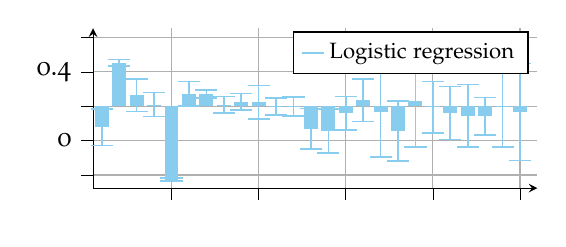
\begin{tikzpicture}

\definecolor{color0}{rgb}{0.533333333333333,0.8,0.933333333333333}

\begin{axis}[
height=1.4222438079424382in,
tick align=outside,
tick pos=left,
width=2.8444876158848764in,
x grid style={white!69.0196078431373!black},
xmajorgrids,
xmin=0.5, xmax=26,
xtick style={color=black},
y grid style={white!69.0196078431373!black},
ymajorgrids,
xticklabels={,,},
ymin=-0.476544751038715, ymax=0.454074936965614,
ytick style={color=black},
yticklabels={-0.4,,0,,0.4},
legend style={font=\footnotesize},
]
\draw[draw=none,fill=color0] (axis cs:0.6,0) rectangle (axis cs:1.4,-0.123064253300487);
\draw[draw=none,fill=color0] (axis cs:1.6,0) rectangle (axis cs:2.4,0.254074936965614);
\draw[draw=none,fill=color0] (axis cs:2.6,0) rectangle (axis cs:3.4,0.0637383003312674);
\draw[draw=none,fill=color0] (axis cs:3.6,0) rectangle (axis cs:4.4,0.010153582132699);
\draw[draw=none,fill=color0] (axis cs:4.6,0) rectangle (axis cs:5.4,-0.426544751038715);
\draw[draw=none,fill=color0] (axis cs:5.6,0) rectangle (axis cs:6.4,0.0732655250272369);
\draw[draw=none,fill=color0] (axis cs:6.6,0) rectangle (axis cs:7.4,0.0708059658830058);
\draw[draw=none,fill=color0] (axis cs:7.6,0) rectangle (axis cs:8.4,0.0083798167350135);
\draw[draw=none,fill=color0] (axis cs:8.6,0) rectangle (axis cs:9.4,0.0258456453297823);
\draw[draw=none,fill=color0] (axis cs:9.6,0) rectangle (axis cs:10.4,0.0225188188581133);
\draw[draw=none,fill=color0] (axis cs:10.6,0) rectangle (axis cs:11.4,-0.00133413758881279);
\draw[draw=none,fill=color0] (axis cs:11.6,0) rectangle (axis cs:12.4,-0.00287012168215015);
\draw[draw=none,fill=color0] (axis cs:12.6,0) rectangle (axis cs:13.4,-0.131874778892413);
\draw[draw=none,fill=color0] (axis cs:13.6,0) rectangle (axis cs:14.4,-0.142790669765573);
\draw[draw=none,fill=color0] (axis cs:14.6,0) rectangle (axis cs:15.4,-0.0405779810634156);
\draw[draw=none,fill=color0] (axis cs:15.6,0) rectangle (axis cs:16.4,0.0350731860669815);
\draw[draw=none,fill=color0] (axis cs:16.6,0) rectangle (axis cs:17.4,-0.0311000025985934);
\draw[draw=none,fill=color0] (axis cs:17.6,0) rectangle (axis cs:18.4,-0.14448078918333);
\draw[draw=none,fill=color0] (axis cs:18.6,0) rectangle (axis cs:19.4,0.033212744542326);
\draw[draw=none,fill=color0] (axis cs:19.6,0) rectangle (axis cs:20.4,-0.00593839297518309);
\draw[draw=none,fill=color0] (axis cs:20.6,0) rectangle (axis cs:21.4,-0.0387638090286288);
\draw[draw=none,fill=color0] (axis cs:21.6,0) rectangle (axis cs:22.4,-0.0546645306377975);
\draw[draw=none,fill=color0] (axis cs:22.6,0) rectangle (axis cs:23.4,-0.057269839782401);
\draw[draw=none,fill=color0] (axis cs:23.6,0) rectangle (axis cs:24.4,-0.0041084420499987);
\draw[draw=none,fill=color0] (axis cs:24.6,0) rectangle (axis cs:25.4,-0.0334022639069669);
\path [draw=color0, semithick]
(axis cs:1,-0.229417488366355)
--(axis cs:1,-0.0167110182346182);

\path [draw=color0, semithick]
(axis cs:2,0.23592009450898)
--(axis cs:2,0.272229779422249);

\path [draw=color0, semithick]
(axis cs:3,-0.0305441203965614)
--(axis cs:3,0.158020721059096);

\path [draw=color0, semithick]
(axis cs:4,-0.0595627687059507)
--(axis cs:4,0.0798699329713486);

\path [draw=color0, semithick]
(axis cs:5,-0.436113887749494)
--(axis cs:5,-0.416975614327935);

\path [draw=color0, semithick]
(axis cs:6,0.00255054819934573)
--(axis cs:6,0.143980501855128);

\path [draw=color0, semithick]
(axis cs:7,0.0465056999066113)
--(axis cs:7,0.0951062318594004);

\path [draw=color0, semithick]
(axis cs:8,-0.0409018572150964)
--(axis cs:8,0.0576614906851234);

\path [draw=color0, semithick]
(axis cs:9,-0.0224725241932268)
--(axis cs:9,0.0741638148527915);

\path [draw=color0, semithick]
(axis cs:10,-0.0756353873903538)
--(axis cs:10,0.12067302510658);

\path [draw=color0, semithick]
(axis cs:11,-0.0502658861107364)
--(axis cs:11,0.0475976109331108);

\path [draw=color0, semithick]
(axis cs:12,-0.0580334518860479)
--(axis cs:12,0.0522932085217476);

\path [draw=color0, semithick]
(axis cs:13,-0.250619578161296)
--(axis cs:13,-0.0131299796235295);

\path [draw=color0, semithick]
(axis cs:14,-0.270974675652396)
--(axis cs:14,-0.0146066638787493);

\path [draw=color0, semithick]
(axis cs:15,-0.137679517728949)
--(axis cs:15,0.0565235556021181);

\path [draw=color0, semithick]
(axis cs:16,-0.0895883476180547)
--(axis cs:16,0.159734719752018);

\path [draw=color0, semithick]
(axis cs:17,-0.293950085783651)
--(axis cs:17,0.231750080586464);

\path [draw=color0, semithick]
(axis cs:18,-0.319655037072536)
--(axis cs:18,0.0306934587058758);

\path [draw=color0, semithick]
(axis cs:19,-0.236206876473511)
--(axis cs:19,0.302632365558163);

\path [draw=color0, semithick]
(axis cs:20,-0.155739313287969)
--(axis cs:20,0.143862527337602);

\path [draw=color0, semithick]
(axis cs:21,-0.192747588063431)
--(axis cs:21,0.115219970006173);

\path [draw=color0, semithick]
(axis cs:22,-0.235981974229328)
--(axis cs:22,0.126652912953733);

\path [draw=color0, semithick]
(axis cs:23,-0.16625366350342)
--(axis cs:23,0.0517139839386183);

\path [draw=color0, semithick]
(axis cs:24,-0.235550284144142)
--(axis cs:24,0.227333400044145);

\path [draw=color0, semithick]
(axis cs:25,-0.315874390637381)
--(axis cs:25,0.249069862823448);

\addplot [semithick, color0, mark=-, mark size=4, mark options={solid}, only marks]
table {%
1 -0.229417488366355
2 0.23592009450898
3 -0.0305441203965614
4 -0.0595627687059507
5 -0.436113887749494
6 0.00255054819934573
7 0.0465056999066113
8 -0.0409018572150964
9 -0.0224725241932268
10 -0.0756353873903538
11 -0.0502658861107364
12 -0.0580334518860479
13 -0.250619578161296
14 -0.270974675652396
15 -0.137679517728949
16 -0.0895883476180547
17 -0.293950085783651
18 -0.319655037072536
19 -0.236206876473511
20 -0.155739313287969
21 -0.192747588063431
22 -0.235981974229328
23 -0.16625366350342
24 -0.235550284144142
25 -0.315874390637381
};
\addplot [semithick, color0, mark=-, mark size=4, mark options={solid}, only marks]
table {%
1 -0.0167110182346182
2 0.272229779422249
3 0.158020721059096
4 0.0798699329713486
5 -0.416975614327935
6 0.143980501855128
7 0.0951062318594004
8 0.0576614906851234
9 0.0741638148527915
10 0.12067302510658
11 0.0475976109331108
12 0.0522932085217476
13 -0.0131299796235295
14 -0.0146066638787493
15 0.0565235556021181
16 0.159734719752018
17 0.231750080586464
18 0.0306934587058758
19 0.302632365558163
20 0.143862527337602
21 0.115219970006173
22 0.126652912953733
23 0.0517139839386183
24 0.227333400044145
25 0.249069862823448
};
\addlegendimage{semithick, color=color0};
\addlegendentry{Logistic regression};
\end{axis}

\end{tikzpicture}

    \label{fig:01-fi-a}
  \end{subfigure}%

  \begin{subfigure}[b]{0.5\textwidth}
    \centering
    % This file was created by tikzplotlib v0.9.8.
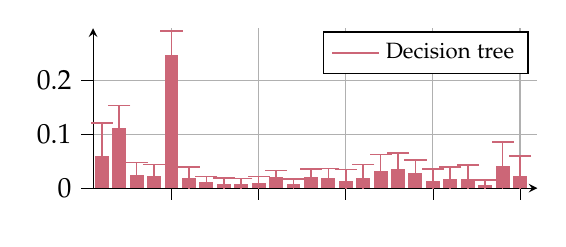
\begin{tikzpicture}

\definecolor{color0}{rgb}{0.8,0.4,0.466666666666667}

\begin{axis}[
height=1.4222438079424382in,
tick align=outside,
tick pos=left,
width=2.8444876158848764in,
x grid style={white!69.0196078431373!black},
xmajorgrids,
xmin=0.5, xmax=26,
xtick style={color=black},
xticklabels={,,},
y grid style={white!69.0196078431373!black},
ymajorgrids,
ymin=0, ymax=0.296093145959793,
ytick style={color=black},
legend style={font=\footnotesize},
]
\draw[draw=none,fill=color0] (axis cs:0.6,0) rectangle (axis cs:1.4,0.0602126647764764);
\draw[draw=none,fill=color0] (axis cs:1.6,0) rectangle (axis cs:2.4,0.110963188395912);
\draw[draw=none,fill=color0] (axis cs:2.6,0) rectangle (axis cs:3.4,0.0240371193898026);
\draw[draw=none,fill=color0] (axis cs:3.6,0) rectangle (axis cs:4.4,0.0221547131912102);
\draw[draw=none,fill=color0] (axis cs:4.6,0) rectangle (axis cs:5.4,0.246093145959793);
\draw[draw=none,fill=color0] (axis cs:5.6,0) rectangle (axis cs:6.4,0.0188217883182872);
\draw[draw=none,fill=color0] (axis cs:6.6,0) rectangle (axis cs:7.4,0.0105015974384699);
\draw[draw=none,fill=color0] (axis cs:7.6,0) rectangle (axis cs:8.4,0.00699136294394965);
\draw[draw=none,fill=color0] (axis cs:8.6,0) rectangle (axis cs:9.4,0.00853041123767904);
\draw[draw=none,fill=color0] (axis cs:9.6,0) rectangle (axis cs:10.4,0.00934264373238672);
\draw[draw=none,fill=color0] (axis cs:10.6,0) rectangle (axis cs:11.4,0.0201245026439328);
\draw[draw=none,fill=color0] (axis cs:11.6,0) rectangle (axis cs:12.4,0.00803736953390133);
\draw[draw=none,fill=color0] (axis cs:12.6,0) rectangle (axis cs:13.4,0.0201541360551478);
\draw[draw=none,fill=color0] (axis cs:13.6,0) rectangle (axis cs:14.4,0.0180446021881651);
\draw[draw=none,fill=color0] (axis cs:14.6,0) rectangle (axis cs:15.4,0.0132118462234375);
\draw[draw=none,fill=color0] (axis cs:15.6,0) rectangle (axis cs:16.4,0.0181046069828721);
\draw[draw=none,fill=color0] (axis cs:16.6,0) rectangle (axis cs:17.4,0.0309174582001746);
\draw[draw=none,fill=color0] (axis cs:17.6,0) rectangle (axis cs:18.4,0.0359878148351983);
\draw[draw=none,fill=color0] (axis cs:18.6,0) rectangle (axis cs:19.4,0.0271294275084838);
\draw[draw=none,fill=color0] (axis cs:19.6,0) rectangle (axis cs:20.4,0.012494436624754);
\draw[draw=none,fill=color0] (axis cs:20.6,0) rectangle (axis cs:21.4,0.0167371542524648);
\draw[draw=none,fill=color0] (axis cs:21.6,0) rectangle (axis cs:22.4,0.0172798021408093);
\draw[draw=none,fill=color0] (axis cs:22.6,0) rectangle (axis cs:23.4,0.00542141841736881);
\draw[draw=none,fill=color0] (axis cs:23.6,0) rectangle (axis cs:24.4,0.0402418644282019);
\draw[draw=none,fill=color0] (axis cs:24.6,0) rectangle (axis cs:25.4,0.0227346258367308);
\path [draw=color0, semithick]
(axis cs:1,5.12811391574566e-05)
--(axis cs:1,0.120374048413795);

\path [draw=color0, semithick]
(axis cs:2,0.0688908846055959)
--(axis cs:2,0.153035492186228);

\path [draw=color0, semithick]
(axis cs:3,0.000443281753072355)
--(axis cs:3,0.0476309570265328);

\path [draw=color0, semithick]
(axis cs:4,0.000463808547678048)
--(axis cs:4,0.0438456178347424);

\path [draw=color0, semithick]
(axis cs:5,0.201175759797789)
--(axis cs:5,0.291010532121796);

\path [draw=color0, semithick]
(axis cs:6,-0.00207540963664902)
--(axis cs:6,0.0397189862732235);

\path [draw=color0, semithick]
(axis cs:7,-0.000261197656391885)
--(axis cs:7,0.0212643925333317);

\path [draw=color0, semithick]
(axis cs:8,-0.00523656669530865)
--(axis cs:8,0.0192192925832079);

\path [draw=color0, semithick]
(axis cs:9,-0.00108881158485408)
--(axis cs:9,0.0181496340602122);

\path [draw=color0, semithick]
(axis cs:10,-0.00317148697566561)
--(axis cs:10,0.0218567744404391);

\path [draw=color0, semithick]
(axis cs:11,0.00759809291557517)
--(axis cs:11,0.0326509123722904);

\path [draw=color0, semithick]
(axis cs:12,-0.00126897867798911)
--(axis cs:12,0.0173437177457918);

\path [draw=color0, semithick]
(axis cs:13,0.00435547873601669)
--(axis cs:13,0.035952793374279);

\path [draw=color0, semithick]
(axis cs:14,-0.000431492489608061)
--(axis cs:14,0.0365206968659383);

\path [draw=color0, semithick]
(axis cs:15,-0.00810189470153616)
--(axis cs:15,0.0345255871484112);

\path [draw=color0, semithick]
(axis cs:16,-0.00758733165253984)
--(axis cs:16,0.0437965456182841);

\path [draw=color0, semithick]
(axis cs:17,-0.000304997596235309)
--(axis cs:17,0.0621399139965845);

\path [draw=color0, semithick]
(axis cs:18,0.00670250518936169)
--(axis cs:18,0.0652731244810349);

\path [draw=color0, semithick]
(axis cs:19,0.00234124172436161)
--(axis cs:19,0.0519176132926061);

\path [draw=color0, semithick]
(axis cs:20,-0.0107608268316967)
--(axis cs:20,0.0357497000812046);

\path [draw=color0, semithick]
(axis cs:21,-0.00616044853556576)
--(axis cs:21,0.0396347570404953);

\path [draw=color0, semithick]
(axis cs:22,-0.00878787812034752)
--(axis cs:22,0.0433474824019661);

\path [draw=color0, semithick]
(axis cs:23,-0.00371385025428554)
--(axis cs:23,0.0145566870890232);

\path [draw=color0, semithick]
(axis cs:24,-0.00489403909324856)
--(axis cs:24,0.0853777679496524);

\path [draw=color0, semithick]
(axis cs:25,-0.0140804363436156)
--(axis cs:25,0.0595496880170773);
\addlegendimage{semithick, color=color0};
\addlegendentry{Decision tree};
\addplot [semithick, color0, mark=-, mark size=0, mark options={solid}, only marks]
table {%
1 5.12811391574566e-05
2 0.0688908846055959
3 0.000443281753072355
4 0.000463808547678048
5 0.201175759797789
6 -0.00207540963664902
7 -0.000261197656391885
8 -0.00523656669530865
9 -0.00108881158485408
10 -0.00317148697566561
11 0.00759809291557517
12 -0.00126897867798911
13 0.00435547873601669
14 -0.000431492489608061
15 -0.00810189470153616
16 -0.00758733165253984
17 -0.000304997596235309
18 0.00670250518936169
19 0.00234124172436161
20 -0.0107608268316967
21 -0.00616044853556576
22 -0.00878787812034752
23 -0.00371385025428554
24 -0.00489403909324856
25 -0.0140804363436156
};
\addplot [semithick, color0, mark=-, mark size=4, mark options={solid}, only marks]
table {%
1 0.120374048413795
2 0.153035492186228
3 0.0476309570265328
4 0.0438456178347424
5 0.291010532121796
6 0.0397189862732235
7 0.0212643925333317
8 0.0192192925832079
9 0.0181496340602122
10 0.0218567744404391
11 0.0326509123722904
12 0.0173437177457918
13 0.035952793374279
14 0.0365206968659383
15 0.0345255871484112
16 0.0437965456182841
17 0.0621399139965845
18 0.0652731244810349
19 0.0519176132926061
20 0.0357497000812046
21 0.0396347570404953
22 0.0433474824019661
23 0.0145566870890232
24 0.0853777679496524
25 0.0595496880170773
};
\end{axis}

\end{tikzpicture}

    \label{fig:01-fi-b}
  \end{subfigure}%

  \begin{subfigure}[b]{0.5\textwidth}
    \centering
    % This file was created by tikzplotlib v0.9.8.
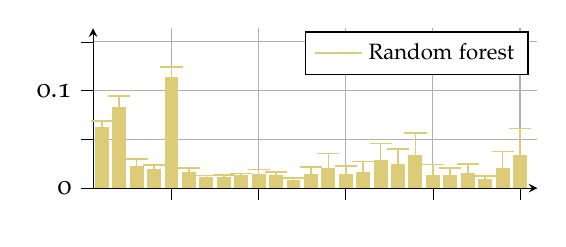
\begin{tikzpicture}

\definecolor{color0}{rgb}{0.866666666666667,0.8,0.466666666666667}

\begin{axis}[
height=1.4222438079424382in,
tick align=outside,
tick pos=left,
width=2.8444876158848764in,
x grid style={white!69.0196078431373!black},
xmajorgrids,
xmin=0.5, xmax=26,
xtick style={color=black},
xticklabels={,,},
y grid style={white!69.0196078431373!black},
ymajorgrids,
ymin=0, ymax=0.163961791193378,
ytick style={color=black},
yticklabels={,0,,0.1,,0.2},
legend style={font=\footnotesize},
]
\draw[draw=none,fill=color0] (axis cs:0.6,0) rectangle (axis cs:1.4,0.0630557431105419);
\draw[draw=none,fill=color0] (axis cs:1.6,0) rectangle (axis cs:2.4,0.0831193744181552);
\draw[draw=none,fill=color0] (axis cs:2.6,0) rectangle (axis cs:3.4,0.022912143158908);
\draw[draw=none,fill=color0] (axis cs:3.6,0) rectangle (axis cs:4.4,0.0195487261065447);
\draw[draw=none,fill=color0] (axis cs:4.6,0) rectangle (axis cs:5.4,0.113961791193378);
\draw[draw=none,fill=color0] (axis cs:5.6,0) rectangle (axis cs:6.4,0.0166845058106126);
\draw[draw=none,fill=color0] (axis cs:6.6,0) rectangle (axis cs:7.4,0.0111880865301946);
\draw[draw=none,fill=color0] (axis cs:7.6,0) rectangle (axis cs:8.4,0.0109815412799707);
\draw[draw=none,fill=color0] (axis cs:8.6,0) rectangle (axis cs:9.4,0.013418791526676);
\draw[draw=none,fill=color0] (axis cs:9.6,0) rectangle (axis cs:10.4,0.0148028536779526);
\draw[draw=none,fill=color0] (axis cs:10.6,0) rectangle (axis cs:11.4,0.0131608319701371);
\draw[draw=none,fill=color0] (axis cs:11.6,0) rectangle (axis cs:12.4,0.00838039909198669);
\draw[draw=none,fill=color0] (axis cs:12.6,0) rectangle (axis cs:13.4,0.0148854194402229);
\draw[draw=none,fill=color0] (axis cs:13.6,0) rectangle (axis cs:14.4,0.0203640215741575);
\draw[draw=none,fill=color0] (axis cs:14.6,0) rectangle (axis cs:15.4,0.0147922332160194);
\draw[draw=none,fill=color0] (axis cs:15.6,0) rectangle (axis cs:16.4,0.0167058216702408);
\draw[draw=none,fill=color0] (axis cs:16.6,0) rectangle (axis cs:17.4,0.0285684173665608);
\draw[draw=none,fill=color0] (axis cs:17.6,0) rectangle (axis cs:18.4,0.0251819365387591);
\draw[draw=none,fill=color0] (axis cs:18.6,0) rectangle (axis cs:19.4,0.0342442655954786);
\draw[draw=none,fill=color0] (axis cs:19.6,0) rectangle (axis cs:20.4,0.0138513854588785);
\draw[draw=none,fill=color0] (axis cs:20.6,0) rectangle (axis cs:21.4,0.0135559278428533);
\draw[draw=none,fill=color0] (axis cs:21.6,0) rectangle (axis cs:22.4,0.0150237331161702);
\draw[draw=none,fill=color0] (axis cs:22.6,0) rectangle (axis cs:23.4,0.0096270211737359);
\draw[draw=none,fill=color0] (axis cs:23.6,0) rectangle (axis cs:24.4,0.0206136662393266);
\draw[draw=none,fill=color0] (axis cs:24.6,0) rectangle (axis cs:25.4,0.0335101355200213);
\path [draw=color0, semithick]
(axis cs:1,0.0573010303012627)
--(axis cs:1,0.0688104559198211);

\path [draw=color0, semithick]
(axis cs:2,0.0715458523831103)
--(axis cs:2,0.0946928964532001);

\path [draw=color0, semithick]
(axis cs:3,0.0162325617369429)
--(axis cs:3,0.0295917245808731);

\path [draw=color0, semithick]
(axis cs:4,0.0151929284504258)
--(axis cs:4,0.0239045237626635);

\path [draw=color0, semithick]
(axis cs:5,0.103650391870818)
--(axis cs:5,0.124273190515939);

\path [draw=color0, semithick]
(axis cs:6,0.0127466082846881)
--(axis cs:6,0.0206224033365371);

\path [draw=color0, semithick]
(axis cs:7,0.00938556140819314)
--(axis cs:7,0.012990611652196);

\path [draw=color0, semithick]
(axis cs:8,0.00854307516043412)
--(axis cs:8,0.0134200073995072);

\path [draw=color0, semithick]
(axis cs:9,0.0116751719811282)
--(axis cs:9,0.0151624110722239);

\path [draw=color0, semithick]
(axis cs:10,0.0103717999049377)
--(axis cs:10,0.0192339074509675);

\path [draw=color0, semithick]
(axis cs:11,0.00968301823796202)
--(axis cs:11,0.0166386457023121);

\path [draw=color0, semithick]
(axis cs:12,0.0064665824303152)
--(axis cs:12,0.0102942157536582);

\path [draw=color0, semithick]
(axis cs:13,0.00834089792296834)
--(axis cs:13,0.0214299409574775);

\path [draw=color0, semithick]
(axis cs:14,0.005070824077227)
--(axis cs:14,0.0356572190710881);

\path [draw=color0, semithick]
(axis cs:15,0.00706511442570956)
--(axis cs:15,0.0225193520063292);

\path [draw=color0, semithick]
(axis cs:16,0.00601575858602535)
--(axis cs:16,0.0273958847544562);

\path [draw=color0, semithick]
(axis cs:17,0.0113173620435266)
--(axis cs:17,0.045819472689595);

\path [draw=color0, semithick]
(axis cs:18,0.0103353119352383)
--(axis cs:18,0.0400285611422799);

\path [draw=color0, semithick]
(axis cs:19,0.011625254341459)
--(axis cs:19,0.0568632768494982);

\path [draw=color0, semithick]
(axis cs:20,0.00342679873482929)
--(axis cs:20,0.0242759721829277);

\path [draw=color0, semithick]
(axis cs:21,0.00673116906011602)
--(axis cs:21,0.0203806866255907);

\path [draw=color0, semithick]
(axis cs:22,0.00496948896783449)
--(axis cs:22,0.0250779772645059);

\path [draw=color0, semithick]
(axis cs:23,0.00660725108889622)
--(axis cs:23,0.0126467912585756);

\path [draw=color0, semithick]
(axis cs:24,0.00380908046748388)
--(axis cs:24,0.0374182520111692);

\path [draw=color0, semithick]
(axis cs:25,0.00587721747702246)
--(axis cs:25,0.0611430535630202);
\addlegendimage{semithick, color=color0};
\addlegendentry{Random forest};
\addplot [semithick, color0, mark=-, mark size=0, mark options={solid}, only marks]
table {%
1 0.0573010303012627
2 0.0715458523831103
3 0.0162325617369429
4 0.0151929284504258
5 0.103650391870818
6 0.0127466082846881
7 0.00938556140819314
8 0.00854307516043412
9 0.0116751719811282
10 0.0103717999049377
11 0.00968301823796202
12 0.0064665824303152
13 0.00834089792296834
14 0.005070824077227
15 0.00706511442570956
16 0.00601575858602535
17 0.0113173620435266
18 0.0103353119352383
19 0.011625254341459
20 0.00342679873482929
21 0.00673116906011602
22 0.00496948896783449
23 0.00660725108889622
24 0.00380908046748388
25 0.00587721747702246
};
\addplot [semithick, color0, mark=-, mark size=4, mark options={solid}, only marks]
table {%
1 0.0688104559198211
2 0.0946928964532001
3 0.0295917245808731
4 0.0239045237626635
5 0.124273190515939
6 0.0206224033365371
7 0.012990611652196
8 0.0134200073995072
9 0.0151624110722239
10 0.0192339074509675
11 0.0166386457023121
12 0.0102942157536582
13 0.0214299409574775
14 0.0356572190710881
15 0.0225193520063292
16 0.0273958847544562
17 0.045819472689595
18 0.0400285611422799
19 0.0568632768494982
20 0.0242759721829277
21 0.0203806866255907
22 0.0250779772645059
23 0.0126467912585756
24 0.0374182520111692
25 0.0611430535630202
};
\end{axis}

\end{tikzpicture}

    \label{fig:01-fi-c}
  \end{subfigure}%

  \begin{subfigure}[b]{0.5\textwidth}
    \centering
    % This file was created by tikzplotlib v0.9.8.
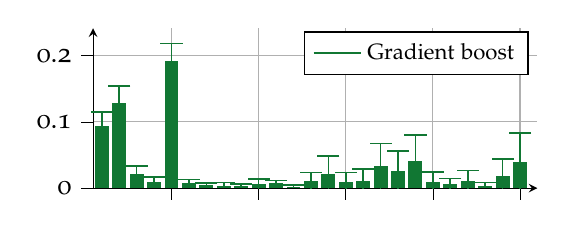
\begin{tikzpicture}

\definecolor{color0}{rgb}{0.0666666666666667,0.466666666666667,0.2}

\begin{axis}[
height=1.4222438079424382in,
tick align=outside,
tick pos=left,
width=2.8444876158848764in,
x grid style={white!69.0196078431373!black},
xmajorgrids,
xmin=0.5, xmax=26,
xtick style={color=black},
xticklabels={,,},
y grid style={white!69.0196078431373!black},
ymajorgrids,
ymin=0, ymax=0.241504672452706,
ytick style={color=black},
yticklabels={,0, 0.1,0.2},
legend style={font=\footnotesize},
]
\draw[draw=none,fill=color0] (axis cs:0.6,0) rectangle (axis cs:1.4,0.0939219294354606);
\draw[draw=none,fill=color0] (axis cs:1.6,0) rectangle (axis cs:2.4,0.128717126999015);
\draw[draw=none,fill=color0] (axis cs:2.6,0) rectangle (axis cs:3.4,0.0213938886864563);
\draw[draw=none,fill=color0] (axis cs:3.6,0) rectangle (axis cs:4.4,0.00888144685168664);
\draw[draw=none,fill=color0] (axis cs:4.6,0) rectangle (axis cs:5.4,0.191504672452706);
\draw[draw=none,fill=color0] (axis cs:5.6,0) rectangle (axis cs:6.4,0.00724897098092836);
\draw[draw=none,fill=color0] (axis cs:6.6,0) rectangle (axis cs:7.4,0.00450287540874152);
\draw[draw=none,fill=color0] (axis cs:7.6,0) rectangle (axis cs:8.4,0.00389892865504545);
\draw[draw=none,fill=color0] (axis cs:8.6,0) rectangle (axis cs:9.4,0.00328938623970718);
\draw[draw=none,fill=color0] (axis cs:9.6,0) rectangle (axis cs:10.4,0.00607634168998537);
\draw[draw=none,fill=color0] (axis cs:10.6,0) rectangle (axis cs:11.4,0.0075927359484662);
\draw[draw=none,fill=color0] (axis cs:11.6,0) rectangle (axis cs:12.4,0.00246964434307127);
\draw[draw=none,fill=color0] (axis cs:12.6,0) rectangle (axis cs:13.4,0.0113273434472604);
\draw[draw=none,fill=color0] (axis cs:13.6,0) rectangle (axis cs:14.4,0.0215526621032538);
\draw[draw=none,fill=color0] (axis cs:14.6,0) rectangle (axis cs:15.4,0.00889067969625317);
\draw[draw=none,fill=color0] (axis cs:15.6,0) rectangle (axis cs:16.4,0.0112833024636162);
\draw[draw=none,fill=color0] (axis cs:16.6,0) rectangle (axis cs:17.4,0.0331145663678211);
\draw[draw=none,fill=color0] (axis cs:17.6,0) rectangle (axis cs:18.4,0.0265656605925389);
\draw[draw=none,fill=color0] (axis cs:18.6,0) rectangle (axis cs:19.4,0.0412663962030667);
\draw[draw=none,fill=color0] (axis cs:19.6,0) rectangle (axis cs:20.4,0.00893277229511404);
\draw[draw=none,fill=color0] (axis cs:20.6,0) rectangle (axis cs:21.4,0.00638009737027819);
\draw[draw=none,fill=color0] (axis cs:21.6,0) rectangle (axis cs:22.4,0.0110083486001703);
\draw[draw=none,fill=color0] (axis cs:22.6,0) rectangle (axis cs:23.4,0.00396903870317716);
\draw[draw=none,fill=color0] (axis cs:23.6,0) rectangle (axis cs:24.4,0.0182603050195842);
\draw[draw=none,fill=color0] (axis cs:24.6,0) rectangle (axis cs:25.4,0.0400563256690563);
\path [draw=color0, semithick]
(axis cs:1,0.0728244166732798)
--(axis cs:1,0.115019442197641);

\path [draw=color0, semithick]
(axis cs:2,0.102746647015722)
--(axis cs:2,0.154687606982308);

\path [draw=color0, semithick]
(axis cs:3,0.0096504157614985)
--(axis cs:3,0.0331373616114142);

\path [draw=color0, semithick]
(axis cs:4,0.00120429954877644)
--(axis cs:4,0.0165585941545968);

\path [draw=color0, semithick]
(axis cs:5,0.164674846558901)
--(axis cs:5,0.218334498346511);

\path [draw=color0, semithick]
(axis cs:6,0.00131865659765555)
--(axis cs:6,0.0131792853642012);

\path [draw=color0, semithick]
(axis cs:7,0.00089826602034204)
--(axis cs:7,0.008107484797141);

\path [draw=color0, semithick]
(axis cs:8,-0.000515167535189504)
--(axis cs:8,0.00831302484528041);

\path [draw=color0, semithick]
(axis cs:9,0.000577548695504199)
--(axis cs:9,0.00600122378391017);

\path [draw=color0, semithick]
(axis cs:10,-0.00123032392384619)
--(axis cs:10,0.0133830073038169);

\path [draw=color0, semithick]
(axis cs:11,0.00341822410793035)
--(axis cs:11,0.0117672477890021);

\path [draw=color0, semithick]
(axis cs:12,0.000427923119383559)
--(axis cs:12,0.00451136556675897);

\path [draw=color0, semithick]
(axis cs:13,-0.000894751232806041)
--(axis cs:13,0.0235494381273268);

\path [draw=color0, semithick]
(axis cs:14,-0.00534323462302397)
--(axis cs:14,0.0484485588295317);

\path [draw=color0, semithick]
(axis cs:15,-0.00580574316011168)
--(axis cs:15,0.023587102552618);

\path [draw=color0, semithick]
(axis cs:16,-0.0063295986999169)
--(axis cs:16,0.0288962036271493);

\path [draw=color0, semithick]
(axis cs:17,-0.000960237853350046)
--(axis cs:17,0.0671893705889922);

\path [draw=color0, semithick]
(axis cs:18,-0.00343303381845922)
--(axis cs:18,0.056564355003537);

\path [draw=color0, semithick]
(axis cs:19,0.00206699809958492)
--(axis cs:19,0.0804657943065485);

\path [draw=color0, semithick]
(axis cs:20,-0.00625580047143954)
--(axis cs:20,0.0241213450616676);

\path [draw=color0, semithick]
(axis cs:21,-0.00190515682114497)
--(axis cs:21,0.0146653515617014);

\path [draw=color0, semithick]
(axis cs:22,-0.00451438685233842)
--(axis cs:22,0.0265310840526791);

\path [draw=color0, semithick]
(axis cs:23,-0.000399848870586143)
--(axis cs:23,0.00833792627694046);

\path [draw=color0, semithick]
(axis cs:24,-0.0070765748506951)
--(axis cs:24,0.0435971848898635);

\path [draw=color0, semithick]
(axis cs:25,-0.00342720675075281)
--(axis cs:25,0.0835398580888655);
\addlegendimage{semithick, color=color0};
\addlegendentry{Gradient boost};
\addplot [semithick, color0, mark=-, mark size=0, mark options={solid}, only marks]
table {%
1 0.0728244166732798
2 0.102746647015722
3 0.0096504157614985
4 0.00120429954877644
5 0.164674846558901
6 0.00131865659765555
7 0.00089826602034204
8 -0.000515167535189504
9 0.000577548695504199
10 -0.00123032392384619
11 0.00341822410793035
12 0.000427923119383559
13 -0.000894751232806041
14 -0.00534323462302397
15 -0.00580574316011168
16 -0.0063295986999169
17 -0.000960237853350046
18 -0.00343303381845922
19 0.00206699809958492
20 -0.00625580047143954
21 -0.00190515682114497
22 -0.00451438685233842
23 -0.000399848870586143
24 -0.0070765748506951
25 -0.00342720675075281
};
\addplot [semithick, color0, mark=-, mark size=4, mark options={solid}, only marks]
table {%
1 0.115019442197641
2 0.154687606982308
3 0.0331373616114142
4 0.0165585941545968
5 0.218334498346511
6 0.0131792853642012
7 0.008107484797141
8 0.00831302484528041
9 0.00600122378391017
10 0.0133830073038169
11 0.0117672477890021
12 0.00451136556675897
13 0.0235494381273268
14 0.0484485588295317
15 0.023587102552618
16 0.0288962036271493
17 0.0671893705889922
18 0.056564355003537
19 0.0804657943065485
20 0.0241213450616676
21 0.0146653515617014
22 0.0265310840526791
23 0.00833792627694046
24 0.0435971848898635
25 0.0835398580888655
};
\end{axis}

\end{tikzpicture}

    \label{fig:01-fi-d}
  \end{subfigure}%

  \begin{subfigure}[b]{0.5\textwidth}
    \centering
    % This file was created by tikzplotlib v0.9.8.
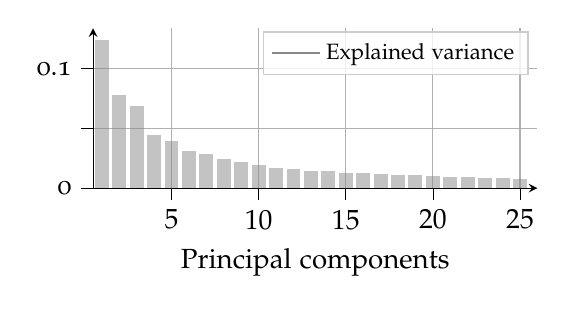
\begin{tikzpicture}

\definecolor{color0}{rgb}{0.8,0.4,0.466666666666667}

\begin{axis}[
height=1.4222438079424382in,
legend style={fill opacity=0.8, draw opacity=1, text opacity=1, draw=white!80!black},
tick align=outside,
tick pos=left,
width=2.8444876158848764in,
x grid style={white!69.0196078431373!black},
xlabel={Principal components},
xmajorgrids,
xmin=0.5, xmax=26,
xtick style={color=black},
y grid style={white!69.0196078431373!black},
ymajorgrids,
ymin=0, ymax=0.133808014644924,
ytick style={color=black},
yticklabels={, 0, , 0.1},
legend style={font=\footnotesize},
]
\draw[draw=none,fill=white!53.3333333333333!black,fill opacity=0.5] (axis cs:0.6,0) rectangle (axis cs:1.4,0.123808014644924);
\draw[draw=none,fill=white!53.3333333333333!black,fill opacity=0.5] (axis cs:1.6,0) rectangle (axis cs:2.4,0.0779020383908885);
\draw[draw=none,fill=white!53.3333333333333!black,fill opacity=0.5] (axis cs:2.6,0) rectangle (axis cs:3.4,0.0690715494994265);
\draw[draw=none,fill=white!53.3333333333333!black,fill opacity=0.5] (axis cs:3.6,0) rectangle (axis cs:4.4,0.0448634890553009);
\draw[draw=none,fill=white!53.3333333333333!black,fill opacity=0.5] (axis cs:4.6,0) rectangle (axis cs:5.4,0.0396017649392185);
\draw[draw=none,fill=white!53.3333333333333!black,fill opacity=0.5] (axis cs:5.6,0) rectangle (axis cs:6.4,0.0309892340254588);
\draw[draw=none,fill=white!53.3333333333333!black,fill opacity=0.5] (axis cs:6.6,0) rectangle (axis cs:7.4,0.0286471759268761);
\draw[draw=none,fill=white!53.3333333333333!black,fill opacity=0.5] (axis cs:7.6,0) rectangle (axis cs:8.4,0.0241373022722755);
\draw[draw=none,fill=white!53.3333333333333!black,fill opacity=0.5] (axis cs:8.6,0) rectangle (axis cs:9.4,0.0219387724823991);
\draw[draw=none,fill=white!53.3333333333333!black,fill opacity=0.5] (axis cs:9.6,0) rectangle (axis cs:10.4,0.0191941500093896);
\draw[draw=none,fill=white!53.3333333333333!black,fill opacity=0.5] (axis cs:10.6,0) rectangle (axis cs:11.4,0.0170987447716404);
\draw[draw=none,fill=white!53.3333333333333!black,fill opacity=0.5] (axis cs:11.6,0) rectangle (axis cs:12.4,0.0163324377943715);
\draw[draw=none,fill=white!53.3333333333333!black,fill opacity=0.5] (axis cs:12.6,0) rectangle (axis cs:13.4,0.0142479118996461);
\draw[draw=none,fill=white!53.3333333333333!black,fill opacity=0.5] (axis cs:13.6,0) rectangle (axis cs:14.4,0.0139471831901937);
\draw[draw=none,fill=white!53.3333333333333!black,fill opacity=0.5] (axis cs:14.6,0) rectangle (axis cs:15.4,0.0125561362477749);
\draw[draw=none,fill=white!53.3333333333333!black,fill opacity=0.5] (axis cs:15.6,0) rectangle (axis cs:16.4,0.0122752355665442);
\draw[draw=none,fill=white!53.3333333333333!black,fill opacity=0.5] (axis cs:16.6,0) rectangle (axis cs:17.4,0.0117377683648439);
\draw[draw=none,fill=white!53.3333333333333!black,fill opacity=0.5] (axis cs:17.6,0) rectangle (axis cs:18.4,0.0108124054147357);
\draw[draw=none,fill=white!53.3333333333333!black,fill opacity=0.5] (axis cs:18.6,0) rectangle (axis cs:19.4,0.0105912984624588);
\draw[draw=none,fill=white!53.3333333333333!black,fill opacity=0.5] (axis cs:19.6,0) rectangle (axis cs:20.4,0.00987028371434172);
\draw[draw=none,fill=white!53.3333333333333!black,fill opacity=0.5] (axis cs:20.6,0) rectangle (axis cs:21.4,0.00946157777094173);
\draw[draw=none,fill=white!53.3333333333333!black,fill opacity=0.5] (axis cs:21.6,0) rectangle (axis cs:22.4,0.00932051055389097);
\draw[draw=none,fill=white!53.3333333333333!black,fill opacity=0.5] (axis cs:22.6,0) rectangle (axis cs:23.4,0.00851928669553865);
\draw[draw=none,fill=white!53.3333333333333!black,fill opacity=0.5] (axis cs:23.6,0) rectangle (axis cs:24.4,0.00821174057436937);
\draw[draw=none,fill=white!53.3333333333333!black,fill opacity=0.5] (axis cs:24.6,0) rectangle (axis cs:25.4,0.00796122578616887);
\addlegendimage{semithick, color=white!53.3333333333333!black};
\addlegendentry{Explained variance};
\end{axis}

\end{tikzpicture}

    \label{fig:01-fi-e}
  \end{subfigure}%

  \caption{Five figures visualizing different parameters for the $25$ most principal components ranked in descending order by the explained variance for the Ferrenti approach. The panels show the logistic regression coefficients, decision trees feature importance, random forests feature importance, gradient boosting feature importance, and explained variance that is retained by choosing each of the eigenvectors. }
  \label{fig:01-fi}
\end{figure}


For logistic regression, we have visualized the mean fitted coefficients and the standard deviation in the top panel of Fig.~\ref{fig:01-fi}. Large positive or negative coefficients can be considered increasingly important, where positive (negative) coefficients will contribute to making positive (negative) predictions. In the three next panels, namely for the machine learning methods  decision trees, random forests, and gradient boosting, we visualize the mean impurity-based feature importance, along with the standard deviation. We observe that the single most important feature for all ML methods is the fifth principal component. Selecting the highest values of this eigenvector, we find that the corresponding features originate from the DFT band gap of the elemental solids among the elements in the compound as calculated by Materials Agnostic Platform for Informatics and Exploration (MagPie). 

After the first ten principal components, we observe that the methods adapt the other principal components with varying degrees. The coefficients for the case of logistic regression experience large fluctuations, but the three remaining models find the first and second principal components important in addition to the fifth. In order of importance, we observe that the second component's largest values correspond to the electronegativity, maximum ionic character, and covalent radius among the elements in the composition. The data originates from elemental calculations from MagPie and are aggregated as either minimum, mean, standard deviation, or maximum. While the first principal component encompasses the largest explained variance, it does not provide any specific information on which features it represents.

%We note that looking at feature importance can be regarded as misleading for data involving correlated features, but we consider the analysis safe due to the projection of the original data to orthogonal vectors, known as principal components, which results in uncorrelated features.
%OH: Seb or Oyv, is it correct to say uncorrelated?


\subsubsection*{Extended Ferrenti approach}

\begin{figure}[ht!]
  \begin{subfigure}[b]{1.0\textwidth}
    \centering
    % This file was created by tikzplotlib v0.9.8.
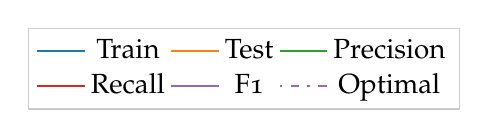
\begin{tikzpicture}

\definecolor{color0}{rgb}{0.12156862745098,0.466666666666667,0.705882352941177}
\definecolor{color1}{rgb}{1,0.498039215686275,0.0549019607843137}
\definecolor{color2}{rgb}{0.172549019607843,0.627450980392157,0.172549019607843}
\definecolor{color3}{rgb}{0.83921568627451,0.152941176470588,0.156862745098039}
\definecolor{color4}{rgb}{0.580392156862745,0.403921568627451,0.741176470588235}
\begin{axis}[%
 hide axis,
 xmin=10,
 xmax=50,
 ymin=0,
 ymax=0.4,
 legend columns=3,
 legend style={
   fill opacity=1,
   draw opacity=1,
   text opacity=1,
   align=center,
   anchor=north,
   draw=white!80!black
 },
 ]
 \addlegendimage{semithick, color0}
 \addlegendentry{Train};
 \addlegendimage{semithick, color1}
 \addlegendentry{Test};
 \addlegendimage{semithick, color2}
 \addlegendentry{Precision};
 \addlegendimage{semithick, color3}
 \addlegendentry{Recall};
 \addlegendimage{semithick, color4}
 \addlegendentry{F1};
 \addlegendimage{semithick, color4, dash pattern=on 1pt off 3pt on 3pt off 3pt}
 \addlegendentry{Optimal};
 \end{axis}

\end{tikzpicture}

  \end{subfigure}
\par\bigskip
  \begin{subfigure}[b]{0.5\textwidth}
    % This file was created by tikzplotlib v0.9.8.
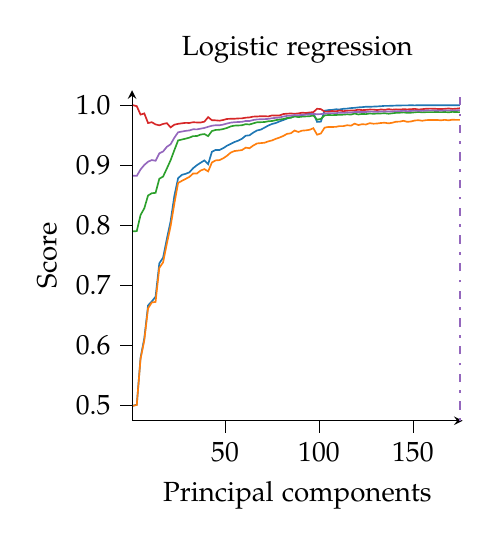
\begin{tikzpicture}

\definecolor{color0}{rgb}{0.12156862745098,0.466666666666667,0.705882352941177}
\definecolor{color1}{rgb}{1,0.498039215686275,0.0549019607843137}
\definecolor{color2}{rgb}{0.172549019607843,0.627450980392157,0.172549019607843}
\definecolor{color3}{rgb}{0.83921568627451,0.152941176470588,0.156862745098039}
\definecolor{color4}{rgb}{0.580392156862745,0.403921568627451,0.741176470588235}

\begin{axis}[
height=2.275590092707901in,
tick align=outside,
tick pos=left,
title={Logistic regression},
width=2.275590092707901in,
x grid style={white!69.0196078431373!black},
xlabel={Principal components},
xmin=0.5, xmax=176.5,
xtick style={color=black},
xtick={0,50,100,150,200},
xticklabels={
  \(\displaystyle {0}\),
  \(\displaystyle {50}\),
  \(\displaystyle {100}\),
  \(\displaystyle {150}\),
  \(\displaystyle {200}\)
},
y grid style={white!69.0196078431373!black},
ylabel={Score},
ymin=0.475, ymax=1.025,
ytick style={color=black},
ytick={0.4,0.5,0.6,0.7,0.8,0.9,1,1.1},
yticklabels={
  \(\displaystyle {0.4}\),
  \(\displaystyle {0.5}\),
  \(\displaystyle {0.6}\),
  \(\displaystyle {0.7}\),
  \(\displaystyle {0.8}\),
  \(\displaystyle {0.9}\),
  \(\displaystyle {1.0}\),
  \(\displaystyle {1.1}\)
}
]
\addplot [semithick, color0]
table {%
1 0.5
3 0.501798443713415
5 0.579650909296173
7 0.612217108576815
9 0.666851932412848
11 0.673572234004334
13 0.681368193243931
15 0.736848953161353
17 0.746388057773118
19 0.777664904121216
21 0.806825109246581
23 0.849063046370876
25 0.878595807810812
27 0.884118929041669
29 0.885853054055898
31 0.888314831682292
33 0.895190977552907
35 0.900235985278826
37 0.904276674778563
39 0.908181782010222
41 0.901870662878299
43 0.922546261062339
45 0.925601164519772
47 0.9254729339368
49 0.928443815030069
51 0.932593869336044
53 0.935674263898019
55 0.938803292222359
57 0.940931671818528
59 0.944199482740069
61 0.949242601454011
63 0.949908815956968
65 0.954414097827993
67 0.957904328647786
69 0.959406992101169
71 0.962625419637909
73 0.966155503695064
75 0.968762829533005
77 0.970375120876515
79 0.973031993958117
81 0.975276019639528
83 0.977727007495695
85 0.979772100329116
87 0.981360407875183
89 0.982209623966871
91 0.98341535632336
93 0.985183311162034
95 0.985502294714261
97 0.986953981289953
99 0.972192562034556
101 0.972663279267337
103 0.990824097958852
105 0.991879743293845
107 0.992246942041616
109 0.993206964364529
111 0.992962039176216
113 0.993985048511097
115 0.994382821134431
117 0.995229420227322
119 0.995645639125988
121 0.996411328896158
123 0.996794213505733
125 0.997425057600618
127 0.997323560429034
129 0.997694720521966
131 0.997954606065713
133 0.998382240061024
135 0.998911889297017
137 0.998890984920851
139 0.999148037709397
141 0.999384366341655
143 0.99950991717191
145 0.999748898339491
147 0.999770097921043
149 0.999814948077676
151 0.999769997150146
153 0.999826867028808
155 0.999871602199933
157 0.999904634176331
159 0.99995230998086
161 0.999952317088165
163 0.99995230998086
165 0.999964243146603
167 0.999988081048868
169 0.999988081048868
171 0.999988081048868
173 0.999988081048868
175 0.999988081048868
};
\addplot [semithick, color1]
table {%
1 0.5
3 0.501166495424849
5 0.577801488498386
7 0.608609443487129
9 0.66200800920252
11 0.671827545667045
13 0.672709384973108
15 0.729370295457408
17 0.738442898916646
19 0.769445095112159
21 0.798578069375205
23 0.83620132048175
25 0.870642838713244
27 0.874130442495001
29 0.877386234000793
31 0.880694073804456
33 0.886351504163557
35 0.88633971305093
37 0.891318288626164
39 0.893662108409125
41 0.8898742025353
43 0.904706415501762
45 0.908207323160187
47 0.908642897841585
49 0.9115525243962
51 0.915820543950019
53 0.921161732137866
55 0.92372038514819
57 0.924508087528374
59 0.925317497688619
61 0.929433990502606
63 0.928419550133154
65 0.932864588420674
67 0.936376701283623
69 0.936964122919374
71 0.937510285259689
73 0.939824180726926
75 0.941403180797572
77 0.944046434945003
79 0.946209279002835
81 0.94883141281411
83 0.952346232526423
85 0.953263182548385
87 0.957869379352076
89 0.955457671787027
91 0.957656457429131
93 0.958183257157601
95 0.959093243857563
97 0.961721527784177
99 0.950893742532167
101 0.952941985882917
103 0.962692816751289
105 0.963816349677328
107 0.963755785362587
109 0.964008548268692
111 0.965213560816186
113 0.965227773887082
115 0.966688994142455
117 0.965937044443011
119 0.969304635354755
121 0.967009836805779
123 0.968425632673246
125 0.967898378347662
127 0.970157104001376
129 0.969208015806464
131 0.96954273059285
133 0.970430799875907
135 0.970822445271729
137 0.969780051019311
139 0.970788907984015
141 0.972508360900962
143 0.972680894327672
145 0.974041822934424
147 0.972281829476937
149 0.97296246425423
151 0.974506904193658
153 0.975052005295442
155 0.974086565426661
157 0.975136020524445
159 0.975417987455577
161 0.975367491852575
163 0.975361567499992
165 0.974904360292785
167 0.97563549067308
169 0.974842187226435
171 0.975897168136428
173 0.975549167135086
175 0.975574926358339
};
\addplot [semithick, color2]
table {%
1 0.790128273460541
3 0.790516290590501
5 0.817269013364316
7 0.828456349624544
9 0.849759324970931
11 0.853549934389484
13 0.85416249568834
15 0.877629608063347
17 0.88124662794522
19 0.894553784639071
21 0.90845361149138
23 0.925177057225219
25 0.941376146872583
27 0.942895548310387
29 0.944356641765346
31 0.946009234935987
33 0.948584823329848
35 0.948662416121254
37 0.951118483664192
39 0.951962590378421
41 0.94861635235387
43 0.957037985583788
45 0.958840795559473
47 0.959155522618094
49 0.960326914906214
51 0.962127183892908
53 0.964722778783831
55 0.966022606030128
57 0.966273540529563
59 0.966645940971706
61 0.968486554117469
63 0.967881897355416
65 0.969807706189211
67 0.971541394510756
69 0.971736441864402
71 0.97201401882385
73 0.973291166509489
75 0.973702084326994
77 0.975085870940189
79 0.976184742911955
81 0.976997840359025
83 0.978665389254305
85 0.979026985590103
87 0.98152384390663
89 0.980141210086004
91 0.980990984129371
93 0.981347649653277
95 0.981657030636286
97 0.982872315974689
99 0.975982630678265
101 0.977157207061612
103 0.983150804675814
105 0.983717632392961
107 0.983446202542585
109 0.983733241611878
111 0.984030963585366
113 0.984290397020427
115 0.984864870666162
117 0.984387933219965
119 0.986082143851482
121 0.984607848995396
123 0.985517289114877
125 0.985155008902799
127 0.986194295953589
129 0.985720314189279
131 0.98608954033897
133 0.986279019082888
135 0.986637809307374
137 0.985815213385238
139 0.986547579347838
141 0.987308045475123
143 0.987491134598958
145 0.988058790183777
147 0.987208365722594
149 0.987497828588714
151 0.988157517340213
153 0.988713446865816
155 0.988062973396862
157 0.988438413638872
159 0.98853893770223
161 0.988537902079904
163 0.988626647742683
165 0.988439632793881
167 0.988716112082819
169 0.988163524325118
171 0.988904523278281
173 0.988627997426313
175 0.988454245385335
};
\addplot [semithick, color3]
table {%
1 1
3 0.998378679395386
5 0.984354585748381
7 0.986359813615184
9 0.970341629730651
11 0.971676326855325
13 0.968050687578134
15 0.966520513694738
17 0.968809864757359
19 0.970145016479146
21 0.963089214683487
23 0.96756995113081
25 0.969001250142062
27 0.969859984089101
29 0.970621888851006
31 0.970432549153313
33 0.971670189794295
35 0.971289464711899
37 0.971195135810888
39 0.972626662120696
41 0.980160245482441
43 0.975008069098761
45 0.974815547221275
47 0.97424525514263
49 0.975389476076827
51 0.977107625866576
53 0.977394249346517
55 0.977489032844641
57 0.977967269007842
59 0.978157517899761
61 0.97920581884305
63 0.979683373110581
65 0.981018752130924
67 0.981209001022843
69 0.981685646096147
71 0.981687237186044
73 0.981305375610865
75 0.983021934310717
77 0.982925559722696
79 0.982926923514036
81 0.985310830776224
83 0.985882941243323
85 0.986262529832935
87 0.985787021252415
89 0.98635935901807
91 0.987504034549381
93 0.987122627571315
95 0.987887259915899
97 0.988459143084441
99 0.994084782361632
101 0.993512671894533
103 0.989317422434367
105 0.989411978633936
107 0.9903654960791
109 0.989793158313445
111 0.991128537333788
113 0.990079099897716
115 0.990842595749517
117 0.991127628139561
119 0.991414933515172
121 0.992558927150813
123 0.991796567791794
125 0.992177065575634
127 0.992749857938402
129 0.992653483350381
131 0.991891123991363
133 0.992940106830322
135 0.992272303670872
137 0.993417888396409
139 0.992559154449369
141 0.993131264916468
143 0.992749176042732
145 0.993321741106944
147 0.99303534492556
149 0.993321968405501
151 0.993894760768269
153 0.992845323332197
155 0.993417661097852
157 0.994084782361632
159 0.994275485850665
161 0.994180929651097
163 0.993799068075918
165 0.993608591885442
167 0.99398977156495
169 0.994562109330606
171 0.993798840777361
173 0.99418070235254
175 0.994943289010115
};
\addplot [semithick, color4]
table {%
1 0.882761362791421
3 0.882369811572774
5 0.893047059725009
7 0.900524634618104
9 0.906005914541491
11 0.908741201904587
13 0.907509532906568
15 0.919898023646594
17 0.92292477913701
19 0.930760618573049
21 0.934928632131644
23 0.945857147607333
25 0.954950144866646
27 0.956153074640595
29 0.957268138593173
31 0.958025004840918
33 0.959931211385276
35 0.959781726571795
37 0.960994581352262
39 0.962136273196524
41 0.964094840986095
43 0.965872246829447
45 0.966685532446835
47 0.966576545346269
49 0.967745382249968
51 0.969505894134768
53 0.970977235787791
55 0.971668429980536
57 0.972048859983711
59 0.972330375537713
61 0.973782397845247
63 0.973711915501329
65 0.975352982408619
67 0.976325230023586
69 0.97666104533464
71 0.97680216205845
73 0.977256877519117
75 0.978316955217665
77 0.97896654484253
79 0.979519324643152
81 0.981107631325292
83 0.982237088649857
85 0.982611039366908
87 0.983632518917407
89 0.983222918403962
91 0.984222240830619
93 0.984214958154773
95 0.984745528462012
97 0.985642934244575
99 0.984934634519006
101 0.985252309073825
103 0.986216216882705
105 0.986547665520533
107 0.986884980548045
109 0.986741006933256
111 0.987556240516879
113 0.987165251924729
115 0.987833525697091
117 0.987737744836704
119 0.988732366828466
121 0.988556767611948
123 0.988640355212257
125 0.988641172840185
127 0.989452159441107
129 0.989165873555307
131 0.988970958030323
133 0.989589182942634
135 0.989441708063597
137 0.98959671779129
139 0.989539786497338
141 0.990205429184222
143 0.990106678858156
145 0.990677783795654
147 0.990107936360012
149 0.990394316734334
151 0.991014486392247
153 0.990768588021226
155 0.990726578521634
157 0.991249565963107
159 0.991393027418662
161 0.991346045278285
163 0.991200189389431
165 0.991010257299128
167 0.991342217584542
169 0.991348320352534
171 0.991340962961706
173 0.991391581113322
175 0.991682248498126
};
\addplot [semithick, color4, dash pattern=on 1pt off 3pt on 3pt off 3pt]
table {%
175 0.475
175 1.025
};
\end{axis}

\end{tikzpicture}

    \caption{}
    \label{fig:q2-LOG}
  \end{subfigure}%
  \hfill
  \begin{subfigure}[b]{0.5\textwidth}
    % This file was created by tikzplotlib v0.9.8.
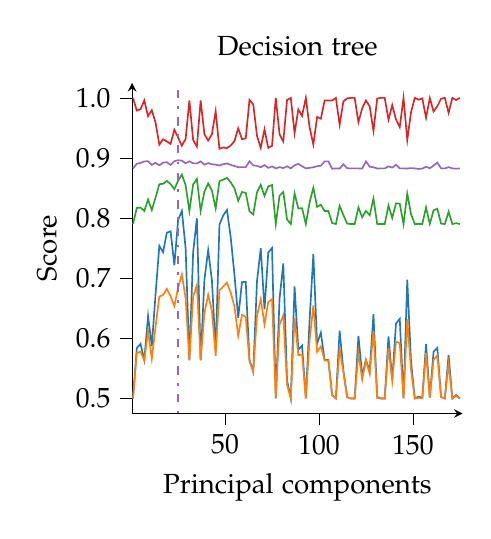
\begin{tikzpicture}

\definecolor{color0}{rgb}{0.12156862745098,0.466666666666667,0.705882352941177}
\definecolor{color1}{rgb}{1,0.498039215686275,0.0549019607843137}
\definecolor{color2}{rgb}{0.172549019607843,0.627450980392157,0.172549019607843}
\definecolor{color3}{rgb}{0.83921568627451,0.152941176470588,0.156862745098039}
\definecolor{color4}{rgb}{0.580392156862745,0.403921568627451,0.741176470588235}

\begin{axis}[
height=2.275590092707901in,
tick align=outside,
tick pos=left,
title={Decision tree},
width=2.275590092707901in,
x grid style={white!69.0196078431373!black},
xlabel={Principal components},
xmin=0.5, xmax=176.5,
xtick style={color=black},
xtick={0,50,100,150,200},
xticklabels={
  \(\displaystyle {0}\),
  \(\displaystyle {50}\),
  \(\displaystyle {100}\),
  \(\displaystyle {150}\),
  \(\displaystyle {200}\)
},
y grid style={white!69.0196078431373!black},
ylabel={Score},
ymin=0.475, ymax=1.025,
ytick style={color=black},
ytick={0.4,0.5,0.6,0.7,0.8,0.9,1,1.1},
yticklabels={
  \(\displaystyle {0.4}\),
  \(\displaystyle {0.5}\),
  \(\displaystyle {0.6}\),
  \(\displaystyle {0.7}\),
  \(\displaystyle {0.8}\),
  \(\displaystyle {0.9}\),
  \(\displaystyle {1.0}\),
  \(\displaystyle {1.1}\)
}
]
\addplot [semithick, color0]
table {%
1 0.5
3 0.583653069490722
5 0.590863668815776
7 0.563897449941446
9 0.637086953758287
11 0.587285485449578
13 0.673439890238702
15 0.753789035271105
17 0.743335533527828
19 0.775797590595263
21 0.778057591395245
23 0.721678708341987
25 0.796683201559861
27 0.811986295217117
29 0.749977941364924
31 0.563897449941446
33 0.743420214578018
35 0.799672922050006
37 0.563897449941446
39 0.697283868431639
41 0.74660791008874
43 0.696719994323555
45 0.578723535104315
47 0.789137121048039
49 0.804400765240516
51 0.81366056721611
53 0.768235828612501
55 0.705752275141642
57 0.634195280080993
59 0.693373832803485
61 0.693963219912857
63 0.563902809103245
65 0.544281410074009
67 0.695178972895485
69 0.750000039715108
71 0.648096076109943
73 0.742735531255245
75 0.750113140478015
77 0.5
79 0.665811170422356
81 0.724546062065308
83 0.529953053857863
85 0.5
87 0.68624558003517
89 0.581142393916758
91 0.587886719019936
93 0.5
95 0.630387044401218
97 0.739994428956417
99 0.591446107231169
101 0.609443240481654
103 0.563897449941446
105 0.563897449941446
107 0.505820148317735
109 0.5
111 0.6126031302384
113 0.545951617563584
115 0.502064224231291
117 0.5
119 0.5
121 0.604140669216679
123 0.538193785652703
125 0.563897449941446
127 0.545638963315292
129 0.640157562207411
131 0.502485102707299
133 0.5
135 0.5
137 0.603055300478667
139 0.531438097342762
141 0.624585947863132
143 0.632344172714643
145 0.5
147 0.697425687818747
149 0.561843658403873
151 0.5
153 0.502964713791134
155 0.501058536781347
157 0.590512127838856
159 0.501931657591992
161 0.577720998335778
163 0.583998300236368
165 0.502354273459707
167 0.5
169 0.572337291531865
171 0.5
173 0.505942706787425
175 0.5
};
\addplot [semithick, color1]
table {%
1 0.5
3 0.575801051562985
5 0.577887567076111
7 0.563234136710867
9 0.612004297171362
11 0.565731532760172
13 0.619597008105958
15 0.669371500293338
17 0.672236905760175
19 0.682402370662514
21 0.669969144220934
23 0.653738104452901
25 0.684861021522716
27 0.706167640364538
29 0.66659096088929
31 0.563234136710867
33 0.669373718757967
35 0.688639822399966
37 0.563234136710867
39 0.641425544364685
41 0.672800775886695
43 0.645307008935291
45 0.571089242327906
47 0.679939216833608
49 0.686130735065103
51 0.692588925184987
53 0.675955344280523
55 0.653128832975492
57 0.603946673915648
59 0.638995439438757
61 0.636038342809226
63 0.561871240742959
65 0.544228945703289
67 0.637266487592263
69 0.665318923679902
71 0.623258205017155
73 0.660301757263571
75 0.66511536630391
77 0.5
79 0.622882654048525
81 0.638452185905646
83 0.522904400223613
85 0.5
87 0.634208857425445
89 0.572142902448988
91 0.572676963444863
93 0.5
95 0.596893188107985
97 0.654608912099962
99 0.577286413075196
101 0.586551721172246
103 0.563234136710867
105 0.563234136710867
107 0.504928834050552
109 0.5
111 0.582722604380719
113 0.54377780030286
115 0.50214157014157
117 0.5
119 0.5
121 0.57622295454336
123 0.531401443806575
125 0.563234136710867
127 0.540860429471408
129 0.612239634878656
131 0.500733552338564
133 0.5
135 0.5
137 0.584201013321538
139 0.528819589449661
141 0.594903056397686
143 0.591970977967398
145 0.5
147 0.631681649941793
149 0.547293912391764
151 0.5
153 0.500725355000415
155 0.500153852710535
157 0.575386703188016
159 0.500938110288946
161 0.564299441275575
163 0.571661772068693
165 0.502216216216216
167 0.5
169 0.557394773822578
171 0.5
173 0.504184041184041
175 0.5
};
\addplot [semithick, color2]
table {%
1 0.790128273460541
3 0.816769966736786
5 0.817555052869596
7 0.811816011439119
9 0.830982576410461
11 0.813343193724055
13 0.834340525569648
15 0.856519110486934
17 0.857113795416815
19 0.861842509799609
21 0.85664017519135
23 0.848249060957542
25 0.862228113626194
27 0.872453248004177
29 0.854674093046235
31 0.811816011439119
33 0.856055340070818
35 0.865044677246367
37 0.811816011439119
39 0.844029937254621
41 0.857779420921906
43 0.845849629714745
45 0.815970412282101
47 0.861537484816431
49 0.864070546113332
51 0.866838967792656
53 0.859478183812805
55 0.849634315896344
57 0.828770671029619
59 0.843433166989528
61 0.842207852810782
63 0.811314485989369
65 0.806165654109346
67 0.842879604420315
69 0.85558949421882
71 0.836971183258513
73 0.85293762725813
75 0.854958200173076
77 0.790128273460541
79 0.837290075732956
81 0.843472931993097
83 0.797927129963984
85 0.790128273460541
87 0.841224997214683
89 0.816032395860042
91 0.816573467250261
93 0.790128273460541
95 0.826117753259477
97 0.850501860562616
99 0.818702918191328
101 0.822244494968421
103 0.811816011439119
105 0.811816011439119
107 0.791903251302414
109 0.790128273460541
111 0.820444939973766
113 0.805134073875265
115 0.790867065597555
117 0.790128273460541
119 0.790128273460541
121 0.817964702882102
123 0.801434258730512
125 0.811816011439119
127 0.804711854952824
129 0.832583749124283
131 0.790372964582338
133 0.790128273460541
135 0.790128273460541
137 0.821056553794393
139 0.800338626104921
141 0.824584189870923
143 0.824134288942085
145 0.790128273460541
147 0.840795816321327
149 0.806883776964119
151 0.790128273460541
153 0.79038157534884
155 0.790180569563684
157 0.817735627803343
159 0.790441277736598
161 0.813108366440122
163 0.815598849668788
165 0.790905025042123
167 0.790128273460541
169 0.810670835126616
171 0.790128273460541
173 0.791608952088033
175 0.790128273460541
};
\addplot [semithick, color3]
table {%
1 1
3 0.978921922945789
5 0.981309239686328
7 0.995802250255711
9 0.969478349812479
11 0.979584043641323
13 0.958881918399818
15 0.922266166609842
17 0.93115013069667
19 0.92750744402773
21 0.923509717013297
23 0.947070803500398
25 0.933901579724969
27 0.920449823843619
29 0.931714740311399
31 0.995802250255711
33 0.930085918854415
35 0.919126491646778
37 0.995802250255711
39 0.939717240595522
41 0.929037845209683
43 0.939529719286283
45 0.977867030344357
47 0.91540288669167
49 0.917596090464825
51 0.916545289237413
53 0.920646209796568
55 0.928191385384703
57 0.949450619388567
59 0.931430389817024
61 0.932565746107512
63 0.996660756904194
65 0.989503579952267
67 0.936958972610524
69 0.917031026252983
71 0.947739061256961
73 0.916935560859189
75 0.920166382543471
77 1
79 0.939709967041709
81 0.927509262416184
83 0.996661438799864
85 1
87 0.9413424252756
89 0.980923514035686
91 0.970144789180589
93 1
95 0.951070803500398
97 0.922451414933515
99 0.968234344811911
101 0.965368564609615
103 0.995802250255711
105 0.995802250255711
107 0.995803614047051
109 1
111 0.955358336174565
113 0.994183657233777
115 0.999238095238095
117 1
119 1
121 0.95957267871349
123 0.982651664961927
125 0.995802250255711
127 0.98569769291965
129 0.945254688032731
131 0.998951017161041
133 1
135 1
137 0.963749516990567
139 0.987896579156722
141 0.96442322991249
143 0.951361518354358
145 1
147 0.929888396408683
149 0.97605500625071
151 1
153 0.997136038186157
155 0.999236276849642
157 0.966992840095465
159 0.999714058415729
161 0.977299011251278
163 0.986161381975224
165 0.998666666666667
167 1
169 0.975108080463689
171 1
173 0.99647619047619
175 1
};
\addplot [semithick, color4]
table {%
1 0.882761362791421
3 0.89046271296871
5 0.891856303774749
7 0.894431074437086
9 0.894550432752301
11 0.888544634370047
13 0.891936346409938
15 0.887927198356199
17 0.892230775065448
19 0.893038346490021
21 0.888573912053492
23 0.894705785551856
25 0.896336548616144
27 0.895633618134226
29 0.89128421722104
31 0.894431074437086
33 0.891195106753311
35 0.891001424349301
37 0.894431074437086
39 0.888915293075693
41 0.891558618585419
43 0.889614918882082
45 0.888957481645236
47 0.887445978650134
49 0.889791147165547
51 0.890863995353364
53 0.88867016697623
55 0.886718083554931
57 0.884658498496669
59 0.884898799983298
61 0.884747226386263
63 0.894473964082037
65 0.88781222734936
67 0.886826486966805
69 0.884684220945597
71 0.888110633400268
73 0.883584929402895
75 0.886066773902887
77 0.882761362791421
79 0.884856422059058
81 0.883099921209487
83 0.886256742039007
85 0.882761362791421
87 0.887830965180748
89 0.890318271655649
91 0.886236618078811
93 0.882761362791421
95 0.883673648194862
97 0.884649465788203
99 0.886379622794579
101 0.887164018720822
103 0.894431074437086
105 0.894431074437086
107 0.882112958218172
109 0.882761362791421
111 0.882400410439924
113 0.889663915140661
115 0.882909142195346
117 0.882761362791421
119 0.882761362791421
121 0.882714540060043
123 0.882422557687418
125 0.894431074437086
127 0.885549614997119
129 0.884648769562057
131 0.882503248077368
133 0.882761362791421
135 0.882761362791421
137 0.886077755834734
139 0.884040696297833
141 0.888773601478652
143 0.882828213791375
145 0.882761362791421
147 0.882544029439833
149 0.883216227927895
151 0.882761362791421
153 0.881768685659238
155 0.882493126706
157 0.885501959548576
159 0.882843990837815
161 0.887330434298401
163 0.892395626266503
165 0.882696147708378
167 0.882761362791421
169 0.884860216449209
171 0.882761362791421
173 0.882229513446938
175 0.882761362791421
};
\addplot [semithick, color4, dash pattern=on 1pt off 3pt on 3pt off 3pt]
table {%
25 0.475
25 1.025
};
\end{axis}

\end{tikzpicture}

    \caption{}
    \label{fig:q2-DT}
  \end{subfigure}

  \begin{subfigure}[b]{0.5\textwidth}
    % This file was created by tikzplotlib v0.9.8.
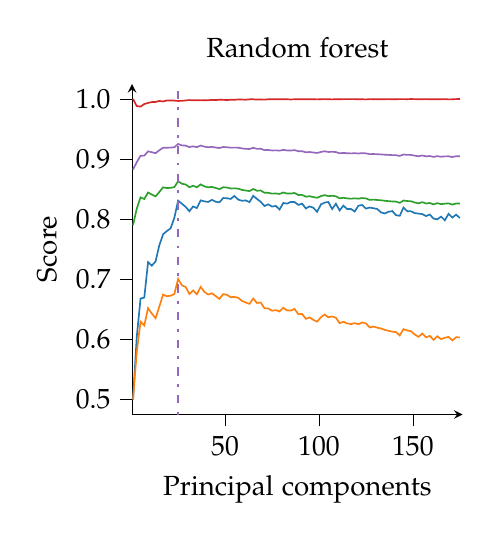
\begin{tikzpicture}

\definecolor{color0}{rgb}{0.12156862745098,0.466666666666667,0.705882352941177}
\definecolor{color1}{rgb}{1,0.498039215686275,0.0549019607843137}
\definecolor{color2}{rgb}{0.172549019607843,0.627450980392157,0.172549019607843}
\definecolor{color3}{rgb}{0.83921568627451,0.152941176470588,0.156862745098039}
\definecolor{color4}{rgb}{0.580392156862745,0.403921568627451,0.741176470588235}

\begin{axis}[
height=2.275590092707901in,
tick align=outside,
tick pos=left,
title={Random forest},
width=2.275590092707901in,
x grid style={white!69.0196078431373!black},
xlabel={Principal components},
xmin=0.5, xmax=176.5,
xtick style={color=black},
xtick={0,50,100,150,200},
xticklabels={
  \(\displaystyle {0}\),
  \(\displaystyle {50}\),
  \(\displaystyle {100}\),
  \(\displaystyle {150}\),
  \(\displaystyle {200}\)
},
y grid style={white!69.0196078431373!black},
ylabel={Score},
ymin=0.475, ymax=1.025,
ytick style={color=black},
ytick={0.4,0.5,0.6,0.7,0.8,0.9,1,1.1},
yticklabels={
  \(\displaystyle {0.4}\),
  \(\displaystyle {0.5}\),
  \(\displaystyle {0.6}\),
  \(\displaystyle {0.7}\),
  \(\displaystyle {0.8}\),
  \(\displaystyle {0.9}\),
  \(\displaystyle {1.0}\),
  \(\displaystyle {1.1}\)
}
]
\addplot [semithick, color0]
table {%
1 0.5
3 0.604667716945488
5 0.66795053446532
7 0.669630095346977
9 0.728494794046075
11 0.722681846477371
13 0.729678679301409
15 0.756602814108593
17 0.774883067682027
19 0.780198694824917
21 0.784757741177697
23 0.802305969567986
25 0.830786263080552
27 0.825736721876078
29 0.820567460338786
31 0.813263001950336
33 0.821160916968535
35 0.818451470435362
37 0.831327352797876
39 0.829672007544245
41 0.828672141885423
43 0.832195540341299
45 0.829023199706599
47 0.828054634641539
49 0.835205567045586
51 0.834797646453054
53 0.833699400413161
55 0.838745346357321
57 0.832535698090392
59 0.830647352244672
61 0.831267972216299
63 0.828363984481282
65 0.838908852723333
67 0.833699299642263
69 0.828811709578274
71 0.821898019851867
73 0.824680505869905
75 0.820999143447372
77 0.822077392049176
79 0.816005413643214
81 0.826925580692296
83 0.825893082077896
85 0.828765254194589
87 0.828451755932886
89 0.823783846425152
91 0.825893082077896
93 0.817858215347408
95 0.821271930266539
97 0.819116340001008
99 0.812249105658286
101 0.824457701415831
103 0.827552980299289
105 0.828631027359299
107 0.816919534438454
109 0.825670277623822
111 0.814537411195647
113 0.822528140273089
115 0.816784803748677
117 0.817050939688618
119 0.812699450798609
121 0.822485312641709
123 0.823557615760568
125 0.817638333249358
127 0.819338136746108
129 0.818223610621252
131 0.816965284425858
133 0.811307300851514
135 0.809469340454477
137 0.812336675568096
139 0.813506121832015
141 0.80668262205875
143 0.805609512772711
145 0.819387917569406
147 0.813325943467527
149 0.813061419861944
151 0.810141986194387
153 0.809242605935406
155 0.808478157907996
157 0.805158462236106
159 0.807807930669623
161 0.800895047110394
163 0.799907391545322
165 0.80425888043533
167 0.797977528089888
169 0.808969819116239
171 0.802687660603618
173 0.807624829949111
175 0.801882098050083
};
\addplot [semithick, color1]
table {%
1 0.5
3 0.579307302273293
5 0.629731425254098
7 0.623077706926156
9 0.651994375128623
11 0.643012015339581
13 0.635348546978619
15 0.654536525956574
17 0.674543774169669
19 0.671823035787236
21 0.672717388032424
23 0.675501701667573
25 0.70064387691476
27 0.69001797808719
29 0.687262224976425
31 0.675560942121801
33 0.681472233484763
35 0.675116263979629
37 0.687357463071664
39 0.679013531175226
41 0.674711615724146
43 0.676799472759497
45 0.672155214966074
47 0.667415530173883
49 0.675389676498865
51 0.674143631954491
53 0.67012627663463
55 0.670780300586983
57 0.669247501251678
59 0.663977988131329
61 0.661312267518115
63 0.659138011690518
65 0.667925012977519
67 0.660563989919002
69 0.661372132275474
71 0.651659000715683
73 0.651462127913799
75 0.647734120584956
77 0.648641342843013
79 0.646422022772858
81 0.652688640140311
83 0.648223597276103
85 0.648036224939566
87 0.650752782103617
89 0.641954519555355
91 0.642362498963334
93 0.634235502038008
95 0.636520572823079
97 0.632479824181495
99 0.629484536787043
101 0.6367565294582
103 0.64138963963964
105 0.636761355713026
107 0.638278086729757
109 0.636075611325611
111 0.62700503435587
113 0.629305341055341
115 0.62667277992278
117 0.625400030101701
119 0.626990233841069
121 0.625391229193735
123 0.628138560739396
125 0.626565182468524
127 0.619846846846847
129 0.621304470256141
131 0.619561548763219
133 0.618141021092692
135 0.615931353532189
137 0.614274131274131
139 0.612871507972343
141 0.612217824967825
143 0.60651243461327
145 0.617112385314056
147 0.614728972579808
149 0.613615508365508
151 0.608129116330787
153 0.604307252359758
155 0.609696683898355
157 0.603463736665407
159 0.60587298387716
161 0.599237110789617
163 0.605165474117145
165 0.600485615687286
167 0.602793852495523
169 0.604164281567623
171 0.598478537180208
173 0.603511583011583
175 0.603367760617761
};
\addplot [semithick, color2]
table {%
1 0.790128273460541
3 0.817707688143582
5 0.836310172529084
7 0.833606413548471
9 0.844423372663908
11 0.840939773806326
13 0.838032566943864
15 0.845229849012221
17 0.852998593909524
19 0.851807480796154
21 0.852139991135229
23 0.853272493523847
25 0.863229151979825
27 0.859013403097388
29 0.857840840037574
31 0.853215365038897
33 0.855591428797773
35 0.853069760753764
37 0.857877732460591
39 0.854631150535879
41 0.852953415402846
43 0.853702199425353
45 0.851919075672918
47 0.850030949701563
49 0.85316601661235
51 0.852665451708983
53 0.851082401690325
55 0.851339158670928
57 0.850722761709645
59 0.848687076803434
61 0.84771208749342
63 0.846790599900558
65 0.850176371481482
67 0.847378302846337
69 0.847670386003156
71 0.843986412376816
73 0.843868476352694
75 0.84248673982235
77 0.842796969712035
79 0.841989697437707
81 0.844363917958259
83 0.842687807328884
85 0.842626093500526
87 0.843605347906096
89 0.840269770793167
91 0.840450111255776
93 0.837406770880754
95 0.838262695115009
97 0.836756026029313
99 0.835640625562135
101 0.838342080478712
103 0.84007116434584
105 0.838331249104115
107 0.838937034780375
109 0.838089994858489
111 0.834729854851567
113 0.835567631409389
115 0.834602471389091
117 0.834099262501438
119 0.834698723814162
121 0.834116034426096
123 0.835150236782934
125 0.834562440414756
127 0.832057054230411
129 0.832604675171445
131 0.831934064855486
133 0.831466320134395
135 0.830664873655185
137 0.830003226727748
139 0.829508382281859
141 0.829259671440244
143 0.827175899739999
145 0.831053669243344
147 0.830209702330862
149 0.829778568303178
151 0.827781126018959
153 0.826371524725482
155 0.828335041796876
157 0.826083465436633
159 0.826949733678646
161 0.824541720651638
163 0.82671757174929
165 0.824984593251849
167 0.825833926765337
169 0.826322423283527
171 0.824270522982255
173 0.826097917396908
175 0.826046317141101
};
\addplot [semithick, color3]
table {%
1 1
3 0.988077281509263
5 0.987313558358904
7 0.991605864302762
9 0.993419252187749
11 0.994849642004773
13 0.994944198204341
15 0.996756449596545
17 0.995802477554268
19 0.997519945448346
21 0.99751971814979
23 0.997329014660757
25 0.99666098420275
27 0.996947153085578
29 0.997519945448346
31 0.99818752130924
33 0.997806114331174
35 0.997996363223093
37 0.997710421638823
39 0.997901579724969
41 0.997901352426412
43 0.998473462893511
45 0.99818752130924
47 0.998759631776338
49 0.998568928287305
51 0.99818752130924
53 0.998759631776338
55 0.998664848278213
57 0.999141720650074
59 0.999046709853392
61 0.998760313672008
63 0.999427889532902
65 0.999427889532902
67 0.999046255256279
69 0.999237186043869
71 0.99885532446869
73 0.999523354926696
75 0.999618820320491
77 0.999618593021934
79 0.999523582225253
81 0.999428116831458
83 0.99952312762814
85 0.999141947948631
87 0.999523582225253
89 0.999523582225253
91 0.999618820320491
93 0.99952312762814
95 0.999427889532902
97 0.999618593021934
99 0.999332651437663
101 0.999523354926696
103 0.999809523809524
105 0.999523354926696
107 0.99933287873622
109 0.999619047619048
111 0.999428344130015
113 0.999714285714286
115 0.999809523809524
117 0.999809069212411
119 0.999714058415729
121 0.999427889532902
123 0.999523582225253
125 0.999237186043869
127 0.999809523809524
129 0.999523354926696
131 0.999618593021934
133 0.999618593021934
135 0.999523582225253
137 0.999809523809524
139 0.999523582225253
141 0.999619047619048
143 0.999714058415729
145 0.999713831117172
147 0.999618820320491
149 0.999904761904762
151 0.999713831117172
153 0.999618365723378
155 0.999618593021934
157 0.999713831117172
159 0.999522673031026
161 0.99952312762814
163 0.999523354926696
165 0.999523354926696
167 0.999809069212411
169 0.999332424139107
171 0.999428116831458
173 0.999809523809524
175 0.999904761904762
};
\addplot [semithick, color4]
table {%
1 0.882761362791421
3 0.894842362678932
5 0.905535642982542
7 0.905752129699778
9 0.912856515144081
11 0.911419154167399
13 0.909752639222031
15 0.914735481640044
17 0.918853234666653
19 0.918894747654292
21 0.919091180355451
23 0.919655230154568
25 0.925110131894938
27 0.922806206891045
29 0.922385580403056
31 0.919995846601909
33 0.921200670055247
35 0.919826331590801
37 0.922486743586808
39 0.92068124453303
41 0.919709092764462
43 0.920392778436662
45 0.919236422138609
47 0.918384436553442
49 0.920117945984395
51 0.919675833696959
53 0.918994231083082
55 0.919105473873538
57 0.91894423962765
59 0.917722131479484
61 0.917023495903923
63 0.916779787763738
65 0.91875628242023
67 0.91695786916923
69 0.917210735574753
71 0.914894328324985
73 0.915104242697119
75 0.914323599448019
77 0.914514278917575
79 0.913994762636924
81 0.915347887315092
83 0.914399871452929
85 0.914206661194271
87 0.914947982300658
89 0.912987622575127
91 0.913126228382476
93 0.911288718952517
95 0.911757202926338
97 0.910942056674186
99 0.910163896979591
101 0.911843780653949
103 0.912981019123732
105 0.911839331816349
107 0.912110796268287
109 0.911733170843149
111 0.909660660411358
113 0.910276703278601
115 0.90973787884528
117 0.90944951123981
119 0.909761195063627
121 0.909300065368489
123 0.909946922459485
125 0.909483939885683
127 0.908231587891891
129 0.908441337410299
131 0.908087581030387
133 0.907791763863255
135 0.907273771012698
137 0.907009945760171
139 0.906595068492627
141 0.906484666700233
143 0.905278887494505
145 0.907594595867454
147 0.907044942460017
149 0.906907709452425
151 0.905636361820386
153 0.904760229634908
155 0.905934307398417
157 0.904620702623776
159 0.905066551108148
161 0.903622189188091
163 0.904919865682502
165 0.903890824813381
167 0.904510182307805
169 0.904615439822114
171 0.903420168762929
173 0.904667306547058
175 0.904676359988818
};
\addplot [semithick, color4, dash pattern=on 1pt off 3pt on 3pt off 3pt]
table {%
25 0.475
25 1.025
};
\end{axis}

\end{tikzpicture}

    \caption{}
    \label{fig:q2-RF}
  \end{subfigure}%
  \hfill
  \begin{subfigure}[b]{0.5\textwidth}
    % This file was created by tikzplotlib v0.9.8.
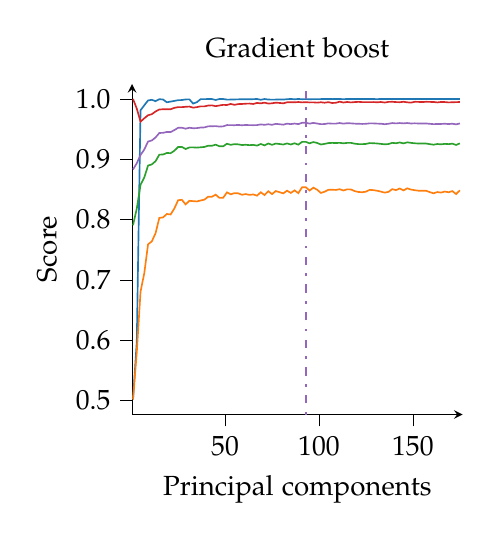
\begin{tikzpicture}

\definecolor{color0}{rgb}{0.12156862745098,0.466666666666667,0.705882352941177}
\definecolor{color1}{rgb}{1,0.498039215686275,0.0549019607843137}
\definecolor{color2}{rgb}{0.172549019607843,0.627450980392157,0.172549019607843}
\definecolor{color3}{rgb}{0.83921568627451,0.152941176470588,0.156862745098039}
\definecolor{color4}{rgb}{0.580392156862745,0.403921568627451,0.741176470588235}

\begin{axis}[
height=2.275590092707901in,
tick align=outside,
tick pos=left,
title={Gradient boost},
width=2.275590092707901in,
x grid style={white!69.0196078431373!black},
xlabel={Principal components},
xmin=0.5, xmax=176.5,
xtick style={color=black},
xtick={0,50,100,150,200},
xticklabels={
  \(\displaystyle {0}\),
  \(\displaystyle {50}\),
  \(\displaystyle {100}\),
  \(\displaystyle {150}\),
  \(\displaystyle {200}\)
},
y grid style={white!69.0196078431373!black},
ylabel={Score},
ymin=0.476460015803393, ymax=1.02493047543793,
ytick style={color=black},
ytick={0.4,0.5,0.6,0.7,0.8,0.9,1,1.1},
yticklabels={
  \(\displaystyle {0.4}\),
  \(\displaystyle {0.5}\),
  \(\displaystyle {0.6}\),
  \(\displaystyle {0.7}\),
  \(\displaystyle {0.8}\),
  \(\displaystyle {0.9}\),
  \(\displaystyle {1.0}\),
  \(\displaystyle {1.1}\)
}
]
\addplot [semithick, color0]
table {%
1 0.501795535849247
3 0.597166345202442
5 0.981358331219243
7 0.989527338228735
9 0.997551614307137
11 0.998608454678289
13 0.996352569384636
15 0.999640953292689
17 0.999102534388069
19 0.994533382960309
21 0.995634173657322
23 0.996810381279227
25 0.997989335100047
27 0.998225771610508
29 0.999236861994256
31 0.999359472191106
33 0.99233989426785
35 0.994680745104805
37 0.999730840933139
39 0.999730639391344
41 0.999910213130448
43 0.999910213130448
45 0.99832736955299
47 0.999955056179775
49 0.999955156950673
51 0.998943757146927
53 0.999012848289414
55 0.999213427175581
57 0.999371794225828
59 0.999640852521792
61 0.999551166423137
63 0.999596110243362
65 0.999685897112914
67 1
69 0.998653801582103
71 0.999955156950673
73 0.999045873158506
75 0.99892275910717
77 0.999000619918284
79 0.999282108127173
81 0.999000929338282
83 0.999641255605381
85 1
87 0.999584184184924
89 0.999955156950673
91 0.999641154834484
93 0.999763664260436
95 0.999596311785157
97 0.999718713332906
99 0.999685897112914
101 0.999820527031793
103 0.999955056179775
105 0.999865470852018
107 0.999820426260896
109 0.999865370081121
111 0.999865470852018
113 0.999775784753363
115 0.999865370081121
117 0.999910213130448
119 1
121 0.999865269310223
123 0.999955156950673
125 0.999865370081121
127 0.999955056179775
129 0.999865370081121
131 0.999775784753363
133 0.999910313901345
135 0.999910313901345
137 1
139 0.999910313901345
141 1
143 0.999910313901345
145 1
147 1
149 0.999955156950673
151 0.999910313901345
153 0.999910213130448
155 0.999955156950673
157 0.999910213130448
159 1
161 0.999955156950673
163 0.999955156950673
165 1
167 1
169 1
171 1
173 0.999955156950673
175 1
};
\addplot [semithick, color1]
table {%
1 0.501390491241327
3 0.579950346783879
5 0.680309122965448
7 0.711077163252581
9 0.75885487524688
11 0.76365529559563
13 0.777257405632704
15 0.802734317935392
17 0.80348554887994
19 0.80921086855693
21 0.808333303385212
23 0.818303287689326
25 0.831984074510924
27 0.832691925218775
29 0.825102914028928
31 0.831045945024465
33 0.830471449458323
35 0.829994048770898
37 0.831578272100945
39 0.832970258444602
41 0.837811673931006
43 0.837775146438631
45 0.841233904804907
47 0.835889953710956
49 0.836057984168963
51 0.845073295337615
53 0.841821252722207
55 0.843770566679875
57 0.843470885819335
59 0.841066123914573
61 0.842207183402291
63 0.840870859864297
65 0.841603674250452
67 0.83959078657587
69 0.845170542260638
71 0.84055304733646
73 0.846953890644821
75 0.842190036183473
77 0.84718547562223
79 0.845337133673053
81 0.84338356017115
83 0.847848774277175
85 0.844155175035247
87 0.848361625092532
89 0.843767371445773
91 0.853530960213538
93 0.85350834323925
95 0.848085638570722
97 0.852813570645313
99 0.849539420173668
101 0.844115599745671
103 0.846076535109948
105 0.849243126522363
107 0.849409754794003
109 0.849074055559139
111 0.850320781999183
113 0.848165868050116
115 0.850086017913584
117 0.849884336518585
119 0.847120766948333
121 0.845692725371126
123 0.845277894754625
125 0.846179495212908
127 0.849233246714154
129 0.848740779818346
131 0.84770667428424
133 0.846267371445772
135 0.844586850317757
137 0.845828504006905
139 0.850433413809309
141 0.84875031867872
143 0.851541067320304
145 0.848263321538381
147 0.851778954457355
149 0.849708680040422
151 0.848622073147133
153 0.847799452026182
155 0.847836888712784
157 0.847720831298397
159 0.845477796156197
161 0.843453135030701
163 0.845579885459957
165 0.844709910984971
167 0.846405799338377
169 0.845235385317128
171 0.847162461643369
173 0.842246665775902
175 0.848442289971526
};
\addplot [semithick, color2]
table {%
1 0.790589797568414
3 0.818055164441743
5 0.857649173873154
7 0.869816750519028
9 0.889530152947373
11 0.891437178351996
13 0.896750314106901
15 0.907587677297353
17 0.907884522712766
19 0.910439831520209
21 0.910049799615289
23 0.914183688596552
25 0.920225916584253
27 0.920509141452369
29 0.916972107855182
31 0.919596395226854
33 0.919699315889372
35 0.919303248416834
37 0.919839047756367
39 0.920433671587121
41 0.922466177610024
43 0.922405698558438
45 0.924160385810301
47 0.921539488847984
49 0.921484058793216
51 0.925671032779082
53 0.923947469921078
55 0.925042785072589
57 0.924702984270113
59 0.923577825419862
61 0.924032485538958
63 0.923394541837552
65 0.92384094162313
67 0.922610444585989
69 0.925328060341464
71 0.923012183158009
73 0.92618589967804
75 0.923917330880262
77 0.926026070142019
79 0.925252011990907
81 0.924461106534393
83 0.926237039805927
85 0.924475706037718
87 0.926492437232025
89 0.924254981888073
91 0.928834225898505
93 0.928801920165306
95 0.92637736300396
97 0.928494385874185
99 0.927067732125062
101 0.924510642024012
103 0.925506286753758
105 0.926820641575909
107 0.927150200274876
109 0.926923437928847
111 0.927227766612082
113 0.92645817419201
115 0.927155509950266
117 0.927209370152734
119 0.925824120305139
121 0.925129188650269
123 0.925040562696919
125 0.925433205772625
127 0.926827725927602
129 0.926554265254949
131 0.926157875483838
133 0.925443909858928
135 0.924784803857116
137 0.925242638350529
139 0.927205293621894
141 0.926554751442286
143 0.927828738939084
145 0.926293384714999
147 0.928047935160069
149 0.927163284097489
151 0.926451424988553
153 0.926102925259818
155 0.926198764323184
157 0.926038982775485
159 0.92503577830514
161 0.924139948155268
163 0.925261406505725
165 0.924732900467042
167 0.925522837695069
169 0.925058209949173
171 0.925911806166609
173 0.923661091768874
175 0.926410301269431
};
\addplot [semithick, color3]
table {%
1 0.999904534606205
3 0.983977270144335
5 0.962420047732697
7 0.967952267303103
9 0.973008978292988
11 0.974723718604387
13 0.979299238549835
15 0.982543925446073
17 0.982926696215479
19 0.982926241618366
21 0.982924650528469
23 0.985309921581998
25 0.986455279008978
27 0.986455279008978
29 0.987026934878964
31 0.987407205364246
33 0.985595408569156
35 0.986455279008978
37 0.987789748835095
39 0.987694056142744
41 0.989123991362655
43 0.989411296738266
45 0.988075917717922
47 0.98921877486078
49 0.990269121491079
51 0.989982498011138
53 0.991795658597568
55 0.990269576088192
57 0.991510626207524
59 0.991701102398
61 0.992178202068417
63 0.992369132856006
65 0.991701556995113
67 0.993419024889192
69 0.992750994431185
71 0.993895669962496
73 0.992369814751676
75 0.992845323332197
77 0.993894760768269
79 0.993418797590635
81 0.992751676326855
83 0.994468462325264
85 0.994658483918627
87 0.994467780429594
89 0.994944652801455
91 0.994372087737243
93 0.99465825662007
95 0.994276167746335
97 0.994372315035799
99 0.993895442663939
101 0.994563245823389
103 0.993800431867258
105 0.994753949312422
107 0.993324014092511
109 0.993704739174906
111 0.995516081372883
113 0.994085918854415
115 0.99504011819525
117 0.994276395044892
119 0.994849642004773
121 0.995230367087169
123 0.994754631208092
125 0.994752812819639
127 0.994753494715309
129 0.994849642004773
131 0.994563927719059
133 0.994944652801455
135 0.994086828048642
137 0.995135128991931
139 0.995326287078077
141 0.994849414706217
143 0.994658711217184
145 0.995326514376634
147 0.994468462325264
149 0.993896124559609
151 0.995326514376634
153 0.995135583589044
155 0.994850096601887
157 0.995325832480964
159 0.995135128991931
161 0.99504011819525
163 0.994277531537675
165 0.99504080009092
167 0.994848278213433
169 0.994277076940562
171 0.994563018524832
173 0.994753949312422
175 0.994944425502898
};
\addplot [semithick, color4]
table {%
1 0.88301188554086
3 0.893361689332264
5 0.906978143803946
7 0.916226891493984
9 0.929367284312758
11 0.931175291841031
13 0.936184019463402
15 0.943550601546772
17 0.943872652911536
19 0.945260014906388
21 0.945049632163219
23 0.948378144871221
25 0.952157887795666
27 0.952318122961393
29 0.950684670967776
31 0.952275260576342
33 0.951464403383461
35 0.951668816769043
37 0.952565905582095
39 0.952853946394613
41 0.954592844522056
43 0.954694874172454
45 0.955018491566572
47 0.954149346001213
49 0.954601766487608
51 0.956705253050836
53 0.956617146614162
55 0.956497517247711
57 0.956905109025401
59 0.956384576744385
61 0.956846919613797
63 0.956595802137781
65 0.956521547393378
67 0.956673364626302
69 0.957806478754475
71 0.957100791562072
73 0.958096456555264
75 0.957099131350643
77 0.958721135088017
79 0.95808890380074
81 0.957354102953769
83 0.959102043878251
85 0.958259018483621
87 0.959234696519263
89 0.958271161511953
91 0.960457458590864
93 0.960569183126699
95 0.959087857477859
97 0.960277132458786
99 0.959288160979858
101 0.958222646963925
103 0.958407483301677
105 0.959549601990439
107 0.959054236739123
109 0.959112488915704
111 0.960118380330598
113 0.959041553807994
115 0.959869486339613
117 0.959533535828149
119 0.959066152994724
121 0.958863479997038
123 0.958589060042731
125 0.95879997539519
127 0.959552812076442
129 0.95946097174585
131 0.959104301384653
133 0.958895709660774
135 0.95815419685312
137 0.95887119427439
139 0.960041371805903
141 0.959459839800619
143 0.960064600007723
145 0.959533225454603
147 0.960076104765857
149 0.959338143849249
151 0.959617993485494
153 0.959347709430662
155 0.959257087361681
157 0.959396559815193
159 0.958772322962232
161 0.958243339088214
163 0.958483037256525
165 0.958556540159858
167 0.958894575428532
169 0.958384296753105
171 0.958972427697617
173 0.957844065348566
175 0.959423321060211
};
\addplot [semithick, color4, dash pattern=on 1pt off 3pt on 3pt off 3pt]
table {%
93 0.476460015803393
93 1.02493047543793
};
\end{axis}

\end{tikzpicture}

    \caption{}
    \label{fig:q2-GB}
  \end{subfigure}
  \caption{Hyperparameter search for the extended Ferrenti approach. The best estimator is visualized for all hyperparameters as a function of principal components during a grid search with a $5\times5$ stratified cross-validation, and the dotted lines mark the optimal hyperparameter combination. Train stands for normal training accuracy, while test is the balanced accuracy on the test set. Precision, recall and F$1$ scores \cite{geron2022,sammut2010} are based on the test set. The number of principal components that explain the $95 \ \%$ accumulated variance is $159$, while the optimal model is found using the F$1$-score.}
  \label{fig:02-pca}
\end{figure}

For the extended Ferrenti approach, the parameter grid search for principal components is visualized in Figure~\ref{fig:02-pca}. All methods experience an almost perfect recall score for the first principal component due to the largely imbalanced dataset with $2141$ suitable and $684$ unsuitable candidates, which results in  a ratio of $75 \ \% : 25 \ \%$. This result comes as a consequence of the ML methods being able to correctly label many suitable candidates compared to the number of unsuitable candidates. 
%On the other hand, we find a small precision for the first component since the ML methods  predict many materials, both actually labeled suitable and unsuitable, as suitable candidates, and the latter case is particularly large. 
On the other hand, we find a low precision score for the first component since the ML methods  predict many materials as suitable regardless of whether they were labeled as suitable or unsuitable in the initial data labeling process, and the latter case is particularly numerous. 
This trend is revealed when looking at the balanced accuracy score. For all figures, it remains the lowest score of the evaluation metrics largely due to the inaccuracy of true negatives for the cross-validations.  

\begin{table}[t]
\centering
\caption{Optimal number of principal components and the respective scores (standard deviation) for each of the four ML methods logistic regression (LOG), decision trees (DT), random forests (RF) and gradient boosting (GB) in the extended Ferrenti approach, as visualized by the dash-dotted line in Fig.~\ref{fig:02-pca}.}
\label{tab:02-pc}
\noindent\makebox[\textwidth]{
\begin{tabular}{M{2.0cm} M{1.5cm} M{2.0cm} M{2.0cm}M{2.0cm}M{2.0cm} }
  \hline
  \hline
   Method & PC & Mean test &  Mean precision & Mean recall & mean F1\\
  \hline
  LOG & $175$ & $0.98(0.008)$ & $0.99(0.004)$ & $0.99(0.004)$ & $0.99(0.003)$ \\
  DT & $25$   & $0.69(0.034)$ & $0.86(0.015)$ & $0.93(0.021)$ & $0.90(0.008)$ \\
  RF & $25$   & $0.70(0.028)$ & $0.86(0.011)$ & $1.00(0.003)$ & $0.93(0.006)$ \\
  GB & $93$   & $0.85(0.025)$ & $0.93(0.011)$ & $0.99(0.004)$ & $0.96(0.007)$ \\
  \hline
\end{tabular}
}
\end{table}

Overall the search for optimal hyperparameters in Fig.~\ref{fig:02-pca} for the extended Ferrenti approach bears resemblance to Fig.~\ref{fig:01-pca} for the Ferrenti approach. Logistic regression performs optimally for many principal components, and is the only method that continues to improve with an increasing number of components. The decision trees method exhibits a large fluctuation of scores, where the number of false positives is dominating the balanced accuracy score. The random forests method exhibits fewer fluctuations compared to decision trees as a consequence of the ensemble decision trees, while gradient boosting does not improve beyond $100$ principal components.


The optimal hyperparameters are summarized in Table~\ref{tab:02-pc}. We find that logistic regression with $175$ principal components performs more or less like a perfect classifier with overall high scores. The decision trees and random forests methods have similar balanced accuracy scores with $0.69$ and $0.70$, respectively, due to challenges associated with predicting true negative labels for $25$ principal components. Lastly, we find that gradient boosting performs optimally at $93$ principal components with a balanced accuracy score of $0.85$. 

The relevant hyperparameters for logistic regression were the regularization strength and the maximum iterations, which were set to $0.46$ and $400$, respectively. Smaller regularization values resulted in worse scores, while increasing values did not noticeably affect the results. The decision trees and random forests methods both found an optimal maximum depth of seven, where smaller values resulted in low precision but high recall.  Therefore, the choice was made to facilitate a compromise between precision and recall. For gradient boosting, we find the optimal maximum depth as four due to a decline in overall metrics for increasing depth except for training accuracy. An increasing depth  could potentially result in overfitting.


The interpretation of feature importance for the extended Ferrenti approach is substantially more difficult than in the Ferrenti approach. We find for logistic regression and decision trees that no feature is different than any other in the cross-validation due to a large variety of accuracy. However, we find that random forests and gradient boosting experience the fifth principal component as important. 
%Similar to the Ferrenti approach, the corresponding features with the highest value for the first principal component originates from the DFT band gap of the elemental solids among the elements in the composition.
Similar to the Ferrenti approach, the extended Ferrenti approach finds the DFT band gap of the elemental solids among the elements in the composition important. The feature regarding the band gap originates from the highest value from the first principal component. 
This means that, if we consider, e.g., the compound SiC, the band gaps of both SiC, Si and C would be considered important by the ML methods. 

\subsubsection*{Empirical approach}

\begin{figure}[ht!]
  \begin{subfigure}[b]{1.0\textwidth}
    \centering
    % This file was created by tikzplotlib v0.9.8.
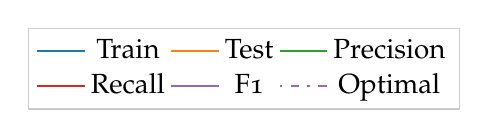
\begin{tikzpicture}

\definecolor{color0}{rgb}{0.12156862745098,0.466666666666667,0.705882352941177}
\definecolor{color1}{rgb}{1,0.498039215686275,0.0549019607843137}
\definecolor{color2}{rgb}{0.172549019607843,0.627450980392157,0.172549019607843}
\definecolor{color3}{rgb}{0.83921568627451,0.152941176470588,0.156862745098039}
\definecolor{color4}{rgb}{0.580392156862745,0.403921568627451,0.741176470588235}
\begin{axis}[%
 hide axis,
 xmin=10,
 xmax=50,
 ymin=0,
 ymax=0.4,
 legend columns=3,
 legend style={
   fill opacity=1,
   draw opacity=1,
   text opacity=1,
   align=center,
   anchor=north,
   draw=white!80!black
 },
 ]
 \addlegendimage{semithick, color0}
 \addlegendentry{Train};
 \addlegendimage{semithick, color1}
 \addlegendentry{Test};
 \addlegendimage{semithick, color2}
 \addlegendentry{Precision};
 \addlegendimage{semithick, color3}
 \addlegendentry{Recall};
 \addlegendimage{semithick, color4}
 \addlegendentry{F1};
 \addlegendimage{semithick, color4, dash pattern=on 1pt off 3pt on 3pt off 3pt}
 \addlegendentry{Optimal};
 \end{axis}

\end{tikzpicture}

  \end{subfigure}
  \par\bigskip
  \begin{subfigure}[b]{0.5\textwidth}
    % This file was created by tikzplotlib v0.9.8.
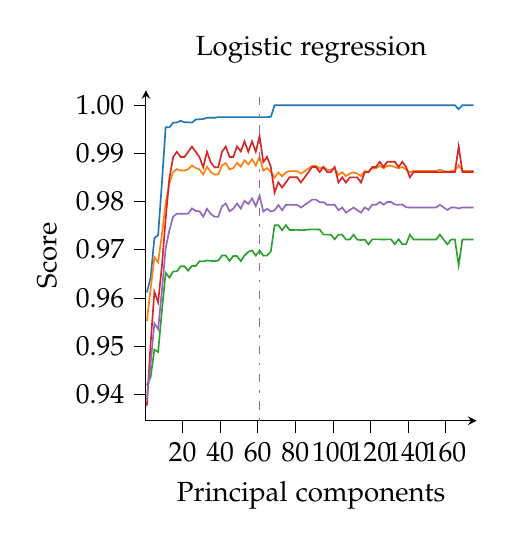
\begin{tikzpicture}

\definecolor{color0}{rgb}{0.12156862745098,0.466666666666667,0.705882352941177}
\definecolor{color1}{rgb}{1,0.498039215686275,0.0549019607843137}
\definecolor{color2}{rgb}{0.172549019607843,0.627450980392157,0.172549019607843}
\definecolor{color3}{rgb}{0.83921568627451,0.152941176470588,0.156862745098039}
\definecolor{color4}{rgb}{0.580392156862745,0.403921568627451,0.741176470588235}

\begin{axis}[
height=2.275590092707901in,
tick align=outside,
tick pos=left,
title={Logistic regression},
width=2.275590092707901in,
x grid style={white!69.0196078431373!black},
xlabel={Principal components},
xmin=0.5, xmax=176.5,
xtick style={color=black},
xtick={0,20,40,60,80,100,120,140,160,180},
xticklabels={
  \(\displaystyle {0}\),
  \(\displaystyle {20}\),
  \(\displaystyle {40}\),
  \(\displaystyle {60}\),
  \(\displaystyle {80}\),
  \(\displaystyle {100}\),
  \(\displaystyle {120}\),
  \(\displaystyle {140}\),
  \(\displaystyle {160}\),
  \(\displaystyle {180}\)
},
y grid style={white!69.0196078431373!black},
ylabel={Score},
ymin=0.934460881934566, ymax=1.00312091038407,
ytick style={color=black},
ytick={0.93,0.94,0.95,0.96,0.97,0.98,0.99,1,1.01},
yticklabels={
  \(\displaystyle {0.93}\),
  \(\displaystyle {0.94}\),
  \(\displaystyle {0.95}\),
  \(\displaystyle {0.96}\),
  \(\displaystyle {0.97}\),
  \(\displaystyle {0.98}\),
  \(\displaystyle {0.99}\),
  \(\displaystyle {1.00}\),
  \(\displaystyle {1.01}\)
}
]
\addplot [semithick, color0]
table {%
1 0.961114291362846
3 0.964184251355771
5 0.97236187869542
7 0.973046537810319
9 0.983798299002821
11 0.995430729241963
13 0.995389702293578
15 0.996361727711372
17 0.996422740268801
19 0.996764027681934
21 0.996454237862116
23 0.996454237862116
25 0.996381022231625
27 0.997022671768936
29 0.99707367974093
31 0.997125594660139
33 0.997384953397758
35 0.997384953397758
37 0.997384953397758
39 0.997519181585678
41 0.997519181585678
43 0.997519181585678
45 0.997519181585678
47 0.997519181585678
49 0.997519181585678
51 0.997519181585678
53 0.997519181585678
55 0.997519181585678
57 0.997519181585678
59 0.997519181585678
61 0.997519181585678
63 0.997519181585678
65 0.997519181585678
67 0.99758129338692
69 1
71 1
73 1
75 1
77 1
79 1
81 1
83 1
85 1
87 1
89 1
91 1
93 1
95 1
97 1
99 1
101 1
103 1
105 1
107 1
109 1
111 1
113 1
115 1
117 1
119 1
121 1
123 1
125 1
127 1
129 1
131 1
133 1
135 1
137 1
139 1
141 1
143 1
145 1
147 1
149 1
151 1
153 1
155 1
157 1
159 1
161 1
163 1
165 1
167 0.999193315770244
169 1
171 1
173 1
175 1
};
\addplot [semithick, color1]
table {%
1 0.95513348875191
3 0.961830387404949
5 0.968449963121016
7 0.967381227718947
9 0.973100732311259
11 0.979723649087684
13 0.983752212739055
15 0.986164374901217
17 0.986719140192824
19 0.986425513232531
21 0.986425513232531
23 0.986719140192824
25 0.987506594313612
27 0.986966053773071
29 0.986672426812778
31 0.985605570482763
33 0.987212967353318
35 0.986131886272237
37 0.985605570482763
39 0.985591345731696
41 0.987462967353318
43 0.988003507893859
45 0.986675513232531
47 0.986925513232531
49 0.988020819064679
51 0.987244503275205
53 0.988547134854152
55 0.987716053773071
57 0.988794048434399
59 0.987466053773071
61 0.98933458897494
63 0.986399197443057
65 0.986939737983598
67 0.986134019984897
69 0.984967818695889
71 0.986034675025903
73 0.985247220905116
75 0.986020450274836
77 0.98631407723513
79 0.98631407723513
81 0.98631407723513
83 0.985773536694589
85 0.98631407723513
87 0.986840393024603
89 0.987380933565144
91 0.987380933565144
93 0.98685461777567
95 0.987145158316211
97 0.986590393024603
99 0.98660461777567
101 0.986884019984897
103 0.985509311943522
105 0.98606407723513
107 0.985259311943522
109 0.985799852484063
111 0.986049852484063
113 0.985799852484063
115 0.985259311943522
117 0.986340393024603
119 0.986093479444357
121 0.986880933565144
123 0.986880933565144
125 0.987421474105684
127 0.986880933565144
129 0.987421474105684
131 0.987421474105684
133 0.987174560525438
135 0.986884019984897
137 0.987174560525438
139 0.986634019984897
141 0.986049852484063
143 0.986357704195423
145 0.986357704195423
147 0.986357704195423
149 0.986357704195423
151 0.986357704195423
153 0.986357704195423
155 0.986357704195423
157 0.986590393024604
159 0.986357704195423
161 0.986110790615176
163 0.986357704195423
165 0.986357704195423
167 0.987535043815745
169 0.986357704195423
171 0.986357704195423
173 0.986357704195423
175 0.986357704195423
};
\addplot [semithick, color2]
table {%
1 0.941849494825663
3 0.943510771845137
5 0.949231831934648
7 0.948739283340263
9 0.957298239140344
11 0.96519952341005
13 0.964188200925043
15 0.96547672368725
17 0.965479380742539
19 0.966533471270313
21 0.966561920772447
23 0.965613202823729
25 0.966640302798197
27 0.966586321691585
29 0.967582054266265
31 0.967553604764131
33 0.967749000012158
35 0.967664988875515
37 0.967607585870744
39 0.967720550510024
41 0.968773182088972
43 0.968773182088972
45 0.967666569403411
47 0.968692210429053
49 0.968661676398519
51 0.967606005342847
53 0.968777558935454
55 0.969542317805476
57 0.96985572211888
59 0.968747528905424
61 0.969830190514401
63 0.968746069956596
65 0.968776099986626
67 0.969633336317547
69 0.975052781667673
71 0.975084527699419
73 0.974030315592575
75 0.975084527699419
77 0.974090375652635
79 0.974085877227084
81 0.974114326729218
83 0.974031896120471
85 0.974085877227084
87 0.97417879244195
89 0.97420882247198
91 0.97420882247198
93 0.974180372969847
95 0.973127741390899
97 0.973127741390899
99 0.973097711360869
101 0.972157540420698
103 0.973097711360869
105 0.973127741390899
107 0.972075109811952
109 0.972101978786189
111 0.973099291888766
113 0.972073529284056
115 0.971988180777654
117 0.972101978786189
119 0.971079377237272
121 0.972132008816219
123 0.972132008816219
125 0.972132008816219
127 0.972103559314086
129 0.972132008816219
131 0.972132008816219
133 0.971133358343885
135 0.972157540420698
137 0.971107826739406
139 0.971107826739406
141 0.973097711360869
143 0.972101978786189
145 0.972101978786189
147 0.972101978786189
149 0.972101978786189
151 0.972101978786189
153 0.972101978786189
155 0.972101978786189
157 0.973127741390899
159 0.972101978786189
161 0.971103328313855
163 0.972101978786189
165 0.972101978786189
167 0.966750227960754
169 0.972101978786189
171 0.972101978786189
173 0.972101978786189
175 0.972101978786189
};
\addplot [semithick, color3]
table {%
1 0.937581792318634
3 0.950469416785206
5 0.961251778093884
7 0.959089615931721
9 0.966571834992888
11 0.976330014224751
13 0.984893314366999
15 0.989217638691323
17 0.990327169274538
19 0.989246088193457
21 0.989246088193457
23 0.990327169274538
25 0.991408250355619
27 0.990327169274538
29 0.989246088193457
31 0.987112375533428
33 0.990327169274538
35 0.988165007112376
37 0.987112375533428
39 0.987083926031294
41 0.990327169274538
43 0.991408250355619
45 0.989246088193457
47 0.989246088193457
49 0.991436699857753
51 0.990384068278805
53 0.9924893314367
55 0.990327169274538
57 0.9924893314367
59 0.990327169274538
61 0.993570412517781
63 0.988193456614509
65 0.98927453769559
67 0.987169274537696
69 0.981849217638691
71 0.98398293029872
73 0.982901849217639
75 0.983954480796586
77 0.985035561877667
79 0.985035561877667
81 0.985035561877667
83 0.983954480796586
85 0.985035561877667
87 0.986088193456614
89 0.987169274537696
91 0.987169274537696
93 0.986116642958748
95 0.987197724039829
97 0.986088193456614
99 0.986116642958748
101 0.987169274537696
103 0.983926031294452
105 0.985035561877667
107 0.983926031294452
109 0.985007112375534
111 0.985007112375533
113 0.985007112375533
115 0.983926031294452
117 0.986088193456615
119 0.986088193456614
121 0.987169274537696
123 0.987169274537696
125 0.988250355618776
127 0.987169274537696
129 0.988250355618776
131 0.988250355618776
133 0.988250355618776
135 0.987169274537696
137 0.988250355618776
139 0.987169274537696
141 0.985007112375533
143 0.986116642958748
145 0.986116642958748
147 0.986116642958748
149 0.986116642958748
151 0.986116642958748
153 0.986116642958748
155 0.986116642958748
157 0.986088193456614
159 0.986116642958748
161 0.986116642958748
163 0.986116642958748
165 0.986116642958748
167 0.991465149359886
169 0.986116642958748
171 0.986116642958748
173 0.986116642958748
175 0.986116642958748
};
\addplot [semithick, color4]
table {%
1 0.938981503311128
3 0.946302105389909
5 0.954717124661412
7 0.95347884635479
9 0.961464763286241
11 0.97027012126079
13 0.974044570892774
15 0.976857799694756
17 0.977468596262435
19 0.977454363716983
21 0.977423081730772
23 0.977496301485237
25 0.978563347478599
27 0.978015979057546
29 0.977987150228718
31 0.976860752073705
33 0.978485010748724
35 0.977405972320794
37 0.976860175289278
39 0.976841372590017
41 0.979003929667643
43 0.979582959401602
45 0.977968924313883
47 0.978488404833364
49 0.979602323701425
51 0.978520681019783
53 0.980131648076607
55 0.979482240504295
57 0.980649990211099
59 0.97902094833577
61 0.981198314743273
63 0.977908388215649
65 0.978471142751006
67 0.9779281626148
69 0.978147632927971
71 0.979273141998686
73 0.97819146854441
75 0.979272549625491
77 0.979316385241929
79 0.97928658471321
81 0.979300999127624
83 0.978739216292157
85 0.97928658471321
87 0.97981823028283
89 0.980380984818187
91 0.980380984818187
93 0.979848837097287
95 0.979863448969433
97 0.979315124437259
99 0.979300694434076
101 0.97932835323924
103 0.97818920399627
105 0.978752337858322
107 0.97768529186496
109 0.978218032825098
111 0.978752155989358
113 0.97821823028283
115 0.977671486278552
117 0.978765978030578
119 0.978262065899269
121 0.979328732565935
123 0.979328732565935
125 0.979891898471567
127 0.979344150723819
129 0.979891898471567
131 0.979891898471567
133 0.979372600225953
135 0.97932835323924
137 0.979372979552648
139 0.978809813647016
141 0.978737149201749
143 0.978766570403773
145 0.978766570403773
147 0.978766570403773
149 0.978766570403773
151 0.978766570403773
153 0.978766570403773
155 0.978766570403773
157 0.979299903737106
159 0.978766570403773
161 0.978247272158159
163 0.978766570403773
165 0.978766570403773
167 0.978544924510936
169 0.978766570403773
171 0.978766570403773
173 0.978766570403773
175 0.978766570403773
};
\addplot [semithick, color4, dash pattern=on 1pt off 3pt on 3pt off 3pt]
table {%
61 0.934460881934566
61 1.00312091038407
};
\end{axis}

\end{tikzpicture}

    \caption{}
    \label{fig:q3-LOG}
  \end{subfigure}%
  \hfill
  \begin{subfigure}[b]{0.5\textwidth}
    % This file was created by tikzplotlib v0.9.8.
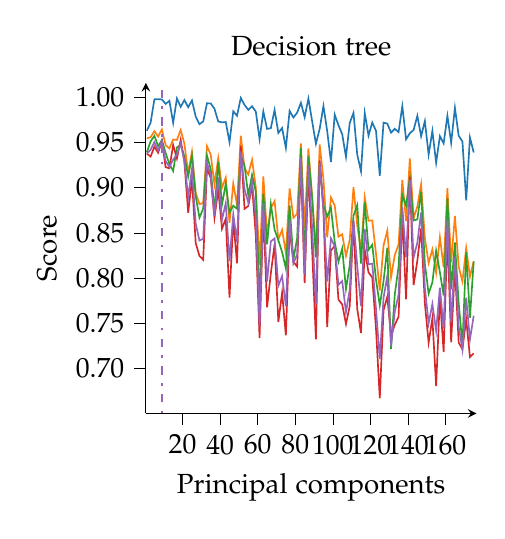
\begin{tikzpicture}

\definecolor{color0}{rgb}{0.12156862745098,0.466666666666667,0.705882352941177}
\definecolor{color1}{rgb}{1,0.498039215686275,0.0549019607843137}
\definecolor{color2}{rgb}{0.172549019607843,0.627450980392157,0.172549019607843}
\definecolor{color3}{rgb}{0.83921568627451,0.152941176470588,0.156862745098039}
\definecolor{color4}{rgb}{0.580392156862745,0.403921568627451,0.741176470588235}

\begin{axis}[
height=2.275590092707901in,
tick align=outside,
tick pos=left,
title={Decision tree},
width=2.275590092707901in,
x grid style={white!69.0196078431373!black},
xlabel={Principal components},
xmin=0.5, xmax=176.5,
xtick style={color=black},
xtick={0,20,40,60,80,100,120,140,160,180},
xticklabels={
  \(\displaystyle {0}\),
  \(\displaystyle {20}\),
  \(\displaystyle {40}\),
  \(\displaystyle {60}\),
  \(\displaystyle {80}\),
  \(\displaystyle {100}\),
  \(\displaystyle {120}\),
  \(\displaystyle {140}\),
  \(\displaystyle {160}\),
  \(\displaystyle {180}\)
},
y grid style={white!69.0196078431373!black},
ylabel={Score},
ymin=0.650360979167302, ymax=1.01576225398736,
ytick style={color=black},
ytick={0.65,0.7,0.75,0.8,0.85,0.9,0.95,1,1.05},
yticklabels={
  \(\displaystyle {0.65}\),
  \(\displaystyle {0.70}\),
  \(\displaystyle {0.75}\),
  \(\displaystyle {0.80}\),
  \(\displaystyle {0.85}\),
  \(\displaystyle {0.90}\),
  \(\displaystyle {0.95}\),
  \(\displaystyle {1.00}\),
  \(\displaystyle {1.05}\)
}
]
\addplot [semithick, color0]
table {%
1 0.962899876599161
3 0.971817014672991
5 0.997580625859956
7 0.997819728594332
9 0.997469151246381
11 0.992544430934772
13 0.995918302743135
15 0.971633048008968
17 0.998469953415844
19 0.98929139355803
21 0.996811533086321
23 0.988858520887424
25 0.996341957960755
27 0.978574755742074
29 0.97006784716152
31 0.973146570131007
33 0.993210655352981
35 0.993035777397751
37 0.98712323230358
39 0.973134597252285
41 0.972110788275519
43 0.972513443626798
45 0.950317607131729
47 0.984375563763799
49 0.979428638601579
51 0.999153105131906
53 0.991409865064539
55 0.985960657071721
57 0.989895519516816
59 0.984006762973347
61 0.95357914910719
63 0.984194038094587
65 0.964869229313987
67 0.965716579949086
69 0.985877935647987
71 0.960441484317804
73 0.965871361409932
75 0.943888029904399
77 0.984815356338938
79 0.977447155312961
81 0.982841125820159
83 0.993720994444854
85 0.977856574896775
87 0.998469953415844
89 0.973217997225243
91 0.948517954002284
93 0.964972277618289
95 0.99019552341751
97 0.962548456867934
99 0.928288649203389
101 0.980610692714958
103 0.968942522829309
105 0.959014256157535
107 0.933999780789552
109 0.971342547390115
111 0.982682709629217
113 0.936453661233926
115 0.918035152303004
117 0.982585251494808
119 0.957437817242952
121 0.971949433099827
123 0.962744890825359
125 0.913166052570346
127 0.971852935401992
129 0.970717030082879
131 0.960832539088155
133 0.964958573843458
135 0.961347743252572
137 0.990025709441291
139 0.953458139540213
141 0.960048995066454
143 0.963703601386711
145 0.97936608254392
147 0.956733679246532
149 0.973593224743808
151 0.936467665295608
153 0.962651283227151
155 0.927517533618132
157 0.956889056554764
159 0.948945937829237
161 0.979338870046423
163 0.949531772467926
165 0.988143406567689
167 0.957379201870335
169 0.950974351359036
171 0.886084106430129
173 0.955430762483149
175 0.938901749863815
};
\addplot [semithick, color1]
table {%
1 0.954395834430922
3 0.955746435031523
5 0.962370304515041
7 0.956384441459003
9 0.964355495846724
11 0.946891338707128
13 0.943331607923713
15 0.953221647085682
17 0.952686958888713
19 0.963701056319477
21 0.948366318072459
23 0.916041361536976
25 0.939592987724567
27 0.894529639288411
29 0.881702421719966
31 0.883037844862406
33 0.945790812742567
35 0.936471291466905
37 0.903506260646612
39 0.932565859719369
41 0.899707119400102
43 0.911180026517746
45 0.861183688074039
47 0.904493216901112
49 0.880604486065012
51 0.957439830181058
53 0.921410313822595
55 0.914473692991237
57 0.930811491315877
59 0.900483321040338
61 0.814699993853503
63 0.912490661714346
65 0.848368996189172
67 0.877337833447483
69 0.885181391918234
71 0.842751764922818
73 0.853240121700648
75 0.827700573380398
77 0.899116932722196
79 0.866622894824649
81 0.87115596737088
83 0.948879691094603
85 0.855034815517272
87 0.943237483097132
89 0.890281404211229
91 0.829254460600952
93 0.947644793916724
95 0.909301599845459
97 0.845132795075778
99 0.889047780236377
101 0.880315425074197
103 0.845663663663664
105 0.848496255026957
107 0.824471809528827
109 0.842302455964737
111 0.900363034086718
113 0.858083947983071
115 0.830367139068893
117 0.889268667790598
119 0.863415274924047
121 0.863708142352879
123 0.826674499060464
125 0.786148644258293
127 0.836109829127373
129 0.85239317387563
131 0.800953387598124
133 0.825595793161583
135 0.837138045940677
137 0.908375186590099
139 0.863116296120682
141 0.932335370458178
143 0.866318467590397
145 0.87910855153399
147 0.903791260558804
149 0.844118921553132
151 0.816679934320285
153 0.831687810617635
155 0.806021477617969
157 0.845243818379783
159 0.811972331981104
161 0.899323916021284
163 0.817381495530618
165 0.868739827546845
167 0.812550440791669
169 0.796429701631456
171 0.833229795585059
173 0.801594375076831
175 0.818620998191174
};
\addplot [semithick, color2]
table {%
1 0.93907670920307
3 0.951116934665084
5 0.957205248408677
7 0.945891200314814
9 0.952596087202494
11 0.938152350415508
13 0.926156760210724
15 0.918280087146029
17 0.94436821023651
19 0.947368064603264
21 0.934391784988002
23 0.912101323843333
25 0.934919829059847
27 0.890651868111788
29 0.866714419955021
31 0.877019001283443
33 0.935488325556797
35 0.920417315504279
37 0.874252872937557
39 0.928730119825786
41 0.88114355727571
43 0.904074385410623
45 0.872363521154313
47 0.879954862512591
49 0.876590260682519
51 0.935894567755249
53 0.924153834308911
55 0.891545604400094
57 0.914108029005937
59 0.895386820052617
61 0.773494041000492
63 0.893117853308747
65 0.837332128889812
67 0.881795957679734
69 0.853555000032216
71 0.841835295229558
73 0.828710226436589
75 0.810625523986733
77 0.880275643028798
79 0.820423751798386
81 0.844206765867607
83 0.944119982031011
85 0.82088585812075
87 0.934455934864529
89 0.889177222123226
91 0.822950119839384
93 0.92780792922666
95 0.880946028106127
97 0.868120774988914
99 0.877772349721532
101 0.840131903304651
103 0.818064177119965
105 0.832662324178584
107 0.787760636675051
109 0.814213480761868
111 0.869085525937458
113 0.880641552264869
115 0.815944067065977
117 0.883860775110761
119 0.831115741302351
121 0.836880693273623
123 0.798061760014802
125 0.76965597909543
127 0.79669251669206
129 0.833588543148054
131 0.721630406961184
133 0.782258527072515
135 0.812593398497749
137 0.892157080186179
139 0.880181310791073
141 0.910201778911495
143 0.863726009401207
145 0.864803660761859
147 0.895613894918624
149 0.815696775354993
151 0.782833636808454
153 0.79529519163656
155 0.830179230585813
157 0.806578048573439
159 0.78082058273829
161 0.888332984254013
163 0.787529555166105
165 0.839292261287652
167 0.772848924853702
169 0.726056737738195
171 0.828584571596553
173 0.756215928648498
175 0.818371484252587
};
\addplot [semithick, color3]
table {%
1 0.937581792318634
3 0.934338549075391
5 0.945092460881935
7 0.938577524893314
9 0.951550497866287
11 0.922560455192034
13 0.921422475106686
15 0.947140825035562
17 0.932176386913229
19 0.95271692745377
21 0.928022759601707
23 0.87226173541963
25 0.909445234708393
27 0.838719772403983
29 0.824466571834993
31 0.820199146514936
33 0.921365576102418
35 0.910640113798009
37 0.866543385490754
39 0.897866287339972
41 0.854537695590327
43 0.865576102418208
45 0.778435277382646
47 0.86452347083926
49 0.816301564722617
51 0.946145092460882
53 0.876586059743954
55 0.879601706970128
57 0.902332859174964
59 0.847083926031295
61 0.733541963015647
63 0.874110953058321
65 0.767596017069701
67 0.805348506401138
69 0.837325746799431
71 0.751522048364154
73 0.783869132290185
75 0.736728307254623
77 0.853826458036985
79 0.818122332859175
81 0.812688477951636
83 0.924580369843528
85 0.794452347083926
87 0.91724039829303
89 0.830241820768137
91 0.732403982930299
93 0.930042674253201
95 0.875220483641536
97 0.745889046941679
99 0.830583214793741
101 0.83547652916074
103 0.776216216216216
105 0.770924608819346
107 0.749246088193457
109 0.769018492176387
111 0.863300142247511
113 0.765803698435278
115 0.739203413940256
117 0.831123755334282
119 0.806287339971551
121 0.80076813655761
123 0.743669985775249
125 0.666970128022759
127 0.764466571834993
129 0.779317211948791
131 0.736443812233286
133 0.74850640113798
135 0.757183499288762
137 0.868904694167852
139 0.776386913229019
141 0.911806543385491
143 0.792204836415363
145 0.819260312944523
147 0.854736842105263
149 0.77203413940256
151 0.728705547652916
153 0.755647226173542
155 0.680512091038407
157 0.779345661450925
159 0.718179231863442
161 0.848221906116643
163 0.729046941678521
165 0.811948790896159
167 0.728847795163585
169 0.721365576102418
171 0.754366998577525
173 0.712830725462304
175 0.716785206258891
};
\addplot [semithick, color4]
table {%
1 0.937491610747551
3 0.94176234518904
5 0.950345855117799
7 0.941093355740073
9 0.951329489482707
11 0.929371450698802
13 0.922891043788085
15 0.930906379382188
17 0.936493691518069
19 0.949058879042792
21 0.929029856112529
23 0.889301298281475
25 0.920575770859652
27 0.860387717662062
29 0.841484289680951
31 0.843501649619401
33 0.927205492563148
35 0.913700034306989
37 0.868759887501304
39 0.91117066861038
41 0.864483653299285
43 0.882837860390343
45 0.818988881857179
47 0.870514121220561
49 0.840244614827214
51 0.939977186446778
53 0.898032953869307
55 0.883384318287348
57 0.906148648212242
59 0.867779987943827
61 0.747468258607015
63 0.882581202523926
65 0.796095836621533
67 0.840614111803912
69 0.843795186854148
71 0.791586903550545
73 0.802212705147121
75 0.768940082368181
77 0.864660498275382
79 0.816347924133622
81 0.826144540099099
83 0.932611450029443
85 0.803932351603323
87 0.92458426957445
89 0.855845125637446
91 0.770848413465091
93 0.927564125378245
95 0.87585438386938
97 0.796051912325468
99 0.843855702216084
101 0.835182887684432
103 0.792590174789401
105 0.796619348383912
107 0.762404828854612
109 0.787161798823522
111 0.864107844346901
113 0.813423402980263
115 0.769477421995406
117 0.854436107309951
119 0.815276675798403
121 0.815944667381948
123 0.76588608752412
125 0.710517654818195
127 0.778088484691358
129 0.802296678933556
131 0.725505636541842
133 0.763017671273528
135 0.781640549400345
137 0.878691141259353
139 0.82303265713603
141 0.908766282968866
143 0.822753892400691
145 0.839077019920646
147 0.872565959059651
149 0.789728485092337
151 0.749875779541732
153 0.771489959095293
155 0.741865726248846
157 0.789479852392897
159 0.744409024714958
161 0.865256449352908
163 0.751145015032122
165 0.823388886582517
167 0.746476705994249
169 0.721003485518006
171 0.778444083467098
173 0.73193123654956
175 0.758339532055329
};
\addplot [semithick, color4, dash pattern=on 1pt off 3pt on 3pt off 3pt]
table {%
9 0.650360979167302
9 1.01576225398736
};
\end{axis}

\end{tikzpicture}

    \caption{}
    \label{fig:q3-DT}
  \end{subfigure}
  \begin{subfigure}[b]{0.5\textwidth}
    % This file was created by tikzplotlib v0.9.8.
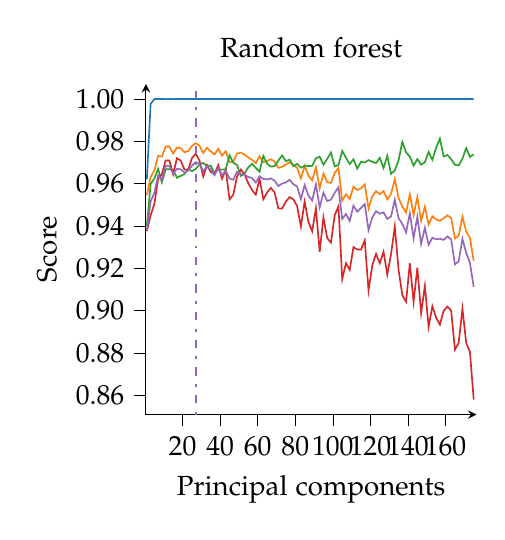
\begin{tikzpicture}

\definecolor{color0}{rgb}{0.12156862745098,0.466666666666667,0.705882352941177}
\definecolor{color1}{rgb}{1,0.498039215686275,0.0549019607843137}
\definecolor{color2}{rgb}{0.172549019607843,0.627450980392157,0.172549019607843}
\definecolor{color3}{rgb}{0.83921568627451,0.152941176470588,0.156862745098039}
\definecolor{color4}{rgb}{0.580392156862745,0.403921568627451,0.741176470588235}

\begin{axis}[
height=2.275590092707901in,
tick align=outside,
tick pos=left,
title={Random forest},
width=2.275590092707901in,
x grid style={white!69.0196078431373!black},
xlabel={Principal components},
xmin=0.5, xmax=176.5,
xtick style={color=black},
xtick={0,20,40,60,80,100,120,140,160,180},
xticklabels={
  \(\displaystyle {0}\),
  \(\displaystyle {20}\),
  \(\displaystyle {40}\),
  \(\displaystyle {60}\),
  \(\displaystyle {80}\),
  \(\displaystyle {100}\),
  \(\displaystyle {120}\),
  \(\displaystyle {140}\),
  \(\displaystyle {160}\),
  \(\displaystyle {180}\)
},
y grid style={white!69.0196078431373!black},
ylabel={Score},
ymin=0.850998577524893, ymax=1.00709530583215,
ytick style={color=black},
ytick={0.84,0.86,0.88,0.9,0.92,0.94,0.96,0.98,1,1.02},
yticklabels={
  \(\displaystyle {0.84}\),
  \(\displaystyle {0.86}\),
  \(\displaystyle {0.88}\),
  \(\displaystyle {0.90}\),
  \(\displaystyle {0.92}\),
  \(\displaystyle {0.94}\),
  \(\displaystyle {0.96}\),
  \(\displaystyle {0.98}\),
  \(\displaystyle {1.00}\),
  \(\displaystyle {1.02}\)
}
]
\addplot [semithick, color0]
table {%
1 0.962075212951391
3 0.99765328816248
5 1
7 1
9 1
11 0.999937888198758
13 1
15 0.999937888198758
17 1
19 1
21 1
23 1
25 1
27 1
29 1
31 1
33 1
35 1
37 1
39 1
41 1
43 1
45 1
47 1
49 1
51 1
53 1
55 1
57 1
59 1
61 1
63 1
65 1
67 1
69 1
71 1
73 1
75 1
77 1
79 1
81 1
83 1
85 1
87 1
89 1
91 1
93 1
95 1
97 1
99 1
101 1
103 1
105 1
107 1
109 1
111 1
113 1
115 1
117 1
119 1
121 1
123 1
125 1
127 1
129 1
131 1
133 1
135 1
137 1
139 1
141 1
143 1
145 1
147 1
149 1
151 1
153 1
155 1
157 1
159 1
161 1
163 1
165 1
167 1
169 1
171 1
173 1
175 1
};
\addplot [semithick, color1]
table {%
1 0.954642748011169
3 0.963096820504715
5 0.966293350367912
7 0.973187362801398
9 0.972777703141738
11 0.977543223047609
13 0.977525911876789
15 0.974271530302232
17 0.977061486925522
19 0.976767859965228
21 0.974869922554133
23 0.975381060885447
25 0.977819538837083
27 0.979136395167097
29 0.978008600705969
31 0.974492128093005
33 0.976919467713327
35 0.975297846091706
37 0.973785755053299
39 0.976447917215461
41 0.973221985143038
43 0.975369922554133
45 0.970097861018914
47 0.970446253270815
49 0.974230989761691
51 0.974637233724953
53 0.973806152643872
55 0.972405128813024
57 0.971297731942469
59 0.969727789192702
61 0.972965812303532
63 0.970115172189734
65 0.970722569060288
67 0.971559822980876
69 0.970483707391602
71 0.967467234778638
73 0.967946837188065
75 0.969085769980507
77 0.970121090388634
79 0.96885403385842
81 0.967522000070246
83 0.962427532795954
85 0.968324631649193
87 0.963772838628102
89 0.961564915792986
91 0.967728373109952
93 0.957730379502309
95 0.96483352211861
97 0.960729795585059
99 0.960378316913405
101 0.96509869957677
103 0.967453962734665
105 0.95200811776689
107 0.95501345204854
109 0.952693763939378
111 0.958592996505277
113 0.957012868131289
115 0.957729453137348
117 0.959675030293451
119 0.94834312382558
121 0.953982170767259
123 0.956474461303409
125 0.95501345204854
127 0.956513122771895
129 0.952595371687477
131 0.955191046309467
133 0.962191757547021
135 0.953230265353072
137 0.949211988304094
139 0.946423836116819
141 0.95501345204854
143 0.945168870625011
145 0.953720079728852
147 0.942474219833869
149 0.949156893735841
151 0.940735942082433
153 0.944606979786804
155 0.943130793073775
157 0.942493739353389
159 0.943761673954656
161 0.945029683191964
163 0.94380743462761
165 0.934107107107107
167 0.935456452066101
169 0.94432261208577
171 0.937458331138156
173 0.934338843229194
175 0.923587065135311
};
\addplot [semithick, color2]
table {%
1 0.939954757983558
3 0.959807662151345
5 0.962506139051031
7 0.966944088033871
9 0.960576738911104
11 0.966802719663401
13 0.966800345704371
15 0.966567239371419
17 0.962805599963495
19 0.963690285077282
21 0.964513921356027
23 0.966984124773598
25 0.965902890701652
27 0.966952604382945
29 0.968947152736626
31 0.9697887592191
33 0.968383168593695
35 0.968498820477509
37 0.964882281312622
39 0.966787621586383
41 0.966625822118082
43 0.966803385181094
45 0.973417028364397
47 0.969908772384344
49 0.968829649733674
51 0.963691782236674
53 0.96474334105913
55 0.967746195176536
57 0.969428551555847
59 0.967455913938886
61 0.965644092591461
63 0.973146230910937
65 0.969399558115088
67 0.968098956566233
69 0.968245574589012
71 0.970957649557061
73 0.973301476171229
75 0.970650112302155
77 0.97133456099746
79 0.968209270104007
81 0.969333132215845
83 0.967564143073431
85 0.968467015538223
87 0.968347477070727
89 0.968397711530838
91 0.972032843104051
93 0.972715117225737
95 0.968952485357842
97 0.971736852781744
99 0.97471281472399
101 0.968170008804468
103 0.968831182428706
105 0.975491992392846
107 0.97223755991403
109 0.969245383608312
111 0.97151879710892
113 0.967100177932005
115 0.970361082223311
117 0.970028118643804
119 0.971137345573104
121 0.9702988432042
123 0.969735293797213
125 0.972207164297287
127 0.967427464789694
129 0.97313141156717
131 0.964618785757331
133 0.966269024447383
135 0.970983676498382
137 0.979740248873376
139 0.974785483654604
141 0.97275913656697
143 0.968542230472149
145 0.971596084202895
147 0.968937546859298
149 0.970140514098569
151 0.974949974016463
153 0.97131590433061
155 0.976905913766379
157 0.981279970208613
159 0.97287969927757
161 0.973526482433528
163 0.9715965669944
165 0.968892196921609
167 0.9686133817075
169 0.971780385546754
171 0.976819290398088
173 0.972622428699054
175 0.973911210751196
};
\addplot [semithick, color3]
table {%
1 0.937581792318634
3 0.945064011379801
5 0.950469416785206
7 0.962275960170697
9 0.964438122332859
11 0.970981507823613
13 0.970953058321479
15 0.964438122332859
17 0.972005689900427
19 0.970924608819346
21 0.966628733997155
23 0.966657183499289
25 0.97203413940256
27 0.974167852062589
29 0.970924608819346
31 0.963385490753912
33 0.96873399715505
35 0.965490753911806
37 0.964466571834993
39 0.968790896159317
41 0.962332859174964
43 0.966628733997155
45 0.952603129445235
47 0.954793741109531
49 0.963357041251778
51 0.966657183499289
53 0.964495021337127
55 0.960199146514936
57 0.956984352773826
59 0.954850640113798
61 0.962332859174964
63 0.952631578947368
65 0.955846372688478
67 0.95800853485064
69 0.955874822190612
71 0.948335704125178
73 0.948307254623044
75 0.951578947368421
77 0.953655761024182
79 0.952603129445235
81 0.949445234708393
83 0.939743954480797
85 0.951550497866287
87 0.941934566145092
89 0.937524893314367
91 0.948364153627311
93 0.927880512091038
95 0.944068278805121
97 0.934366998577525
99 0.932176386913229
101 0.945092460881935
103 0.949302987197724
105 0.914935988620199
107 0.922446657183499
109 0.919288762446657
111 0.930099573257468
113 0.928933143669986
115 0.928847795163585
117 0.93325746799431
119 0.909587482219061
121 0.921365576102418
123 0.926856330014225
125 0.922446657183499
127 0.927908961593172
129 0.917098150782361
131 0.926770981507824
133 0.93977240398293
135 0.919374110953058
137 0.907368421052632
139 0.904267425320057
141 0.922446657183499
143 0.904238975817923
145 0.920341394025605
147 0.898862019914651
149 0.91172119487909
151 0.892403982930299
153 0.902133712660028
155 0.89669985775249
157 0.893456614509246
159 0.899943100995733
161 0.90199146514936
163 0.900028449502134
165 0.881621621621622
167 0.884807965860597
169 0.901052631578947
171 0.884836415362731
173 0.880597439544808
175 0.858093883357041
};
\addplot [semithick, color4]
table {%
1 0.937971131227071
3 0.951696746620232
5 0.955675545223121
7 0.963857057360314
9 0.961893592475637
11 0.968434663574377
13 0.968421121325934
15 0.964804465097189
17 0.967001038409729
19 0.966815627303656
21 0.965197377960728
23 0.966141031671706
25 0.968526219069676
27 0.97013951068787
29 0.969520748025617
31 0.965940162526314
33 0.968244768805547
35 0.966540997354672
37 0.964028581525751
39 0.967341373830983
41 0.963961585502246
43 0.966197465278567
45 0.962384911790855
47 0.961895949952806
49 0.965594498307818
51 0.964655564557004
53 0.964126294663464
55 0.963225241000998
57 0.962595679674952
59 0.960557378081945
61 0.963476794444407
63 0.962245275170185
65 0.962018416064968
67 0.962505686608376
69 0.961441817501155
71 0.958874684190213
73 0.960057084047946
75 0.960588268562161
77 0.961821146268644
79 0.959743796929383
81 0.958686464008725
83 0.952706834216598
85 0.959356920904872
87 0.95440870058703
89 0.952088932691132
91 0.959621121300748
93 0.948812810603067
95 0.955736473035206
97 0.951812035501207
99 0.952441613856118
101 0.955689777608347
103 0.958340165113889
105 0.943314165393577
107 0.945702450617358
109 0.942366589293679
111 0.949603829646948
113 0.946777215077366
115 0.948507173480125
117 0.950404575745889
119 0.938129060505652
121 0.944008262003197
123 0.946995416773745
125 0.945845625884396
127 0.94642484263802
129 0.943407080866632
131 0.94454539238753
133 0.952446155505926
135 0.943669851100656
137 0.941076232860601
139 0.936964376294548
141 0.945987041154613
143 0.934190723875732
145 0.944393782600601
147 0.931506956381904
149 0.939145329371431
151 0.931139472352723
153 0.934489479668438
155 0.933731817808476
157 0.93399205520818
159 0.933455207009215
161 0.935099698485637
163 0.933689135369764
165 0.921910828945626
167 0.923339172012706
169 0.933993810589123
171 0.927374818610162
173 0.922660549168326
175 0.911202322653306
};
\addplot [semithick, color4, dash pattern=on 1pt off 3pt on 3pt off 3pt]
table {%
27 0.850998577524893
27 1.00709530583215
};
\end{axis}

\end{tikzpicture}

    \caption{}
    \label{fig:q3-RF}
  \end{subfigure}%
  \hfill
  \begin{subfigure}[b]{0.5\textwidth}
    % This file was created by tikzplotlib v0.9.8.
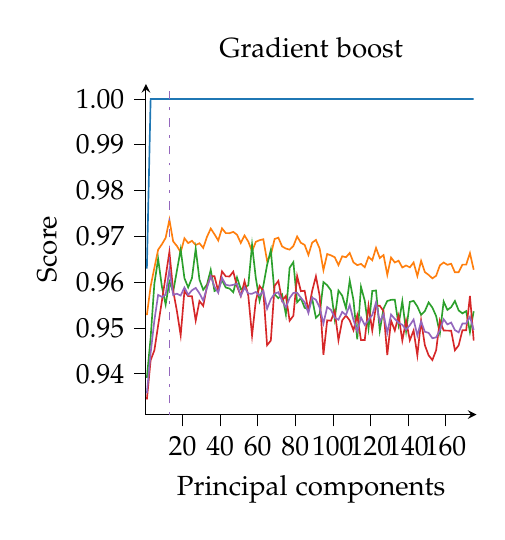
\begin{tikzpicture}

\definecolor{color0}{rgb}{0.12156862745098,0.466666666666667,0.705882352941177}
\definecolor{color1}{rgb}{1,0.498039215686275,0.0549019607843137}
\definecolor{color2}{rgb}{0.172549019607843,0.627450980392157,0.172549019607843}
\definecolor{color3}{rgb}{0.83921568627451,0.152941176470588,0.156862745098039}
\definecolor{color4}{rgb}{0.580392156862745,0.403921568627451,0.741176470588235}

\begin{axis}[
height=2.275590092707901in,
tick align=outside,
tick pos=left,
title={Gradient boost},
width=2.275590092707901in,
x grid style={white!69.0196078431373!black},
xlabel={Principal components},
xmin=0.5, xmax=176.5,
xtick style={color=black},
xtick={0,20,40,60,80,100,120,140,160,180},
xticklabels={
  \(\displaystyle {0}\),
  \(\displaystyle {20}\),
  \(\displaystyle {40}\),
  \(\displaystyle {60}\),
  \(\displaystyle {80}\),
  \(\displaystyle {100}\),
  \(\displaystyle {120}\),
  \(\displaystyle {140}\),
  \(\displaystyle {160}\),
  \(\displaystyle {180}\)
},
y grid style={white!69.0196078431373!black},
ylabel={Score},
ymin=0.931055476529161, ymax=1.00328307254623,
ytick style={color=black},
ytick={0.93,0.94,0.95,0.96,0.97,0.98,0.99,1,1.01},
yticklabels={
  \(\displaystyle {0.93}\),
  \(\displaystyle {0.94}\),
  \(\displaystyle {0.95}\),
  \(\displaystyle {0.96}\),
  \(\displaystyle {0.97}\),
  \(\displaystyle {0.98}\),
  \(\displaystyle {0.99}\),
  \(\displaystyle {1.00}\),
  \(\displaystyle {1.01}\)
}
]
\addplot [semithick, color0]
table {%
1 0.962919717035259
3 1
5 1
7 1
9 1
11 1
13 1
15 1
17 1
19 1
21 1
23 1
25 1
27 1
29 1
31 1
33 1
35 1
37 1
39 1
41 1
43 1
45 1
47 1
49 1
51 1
53 1
55 1
57 1
59 1
61 1
63 1
65 1
67 1
69 1
71 1
73 1
75 1
77 1
79 1
81 1
83 1
85 1
87 1
89 1
91 1
93 1
95 1
97 1
99 1
101 1
103 1
105 1
107 1
109 1
111 1
113 1
115 1
117 1
119 1
121 1
123 1
125 1
127 1
129 1
131 1
133 1
135 1
137 1
139 1
141 1
143 1
145 1
147 1
149 1
151 1
153 1
155 1
157 1
159 1
161 1
163 1
165 1
167 1
169 1
171 1
173 1
175 1
};
\addplot [semithick, color1]
table {%
1 0.9527742128093
3 0.959037344361906
5 0.963111045255782
7 0.967065627030539
9 0.968246053070615
11 0.969652995100364
13 0.973611870642572
15 0.968875981244402
17 0.967883436067647
19 0.966484545949458
21 0.969559822980876
23 0.968519282440335
25 0.969005057689268
27 0.96808885640026
29 0.968475655480041
31 0.96746168536958
33 0.969862709200428
35 0.97168453102225
37 0.970446876701263
39 0.969072168659888
41 0.97173433082205
43 0.97069379028151
45 0.97067647911069
47 0.970955881319916
49 0.970345398029609
51 0.968539680030908
53 0.970167474492036
55 0.968838527123615
57 0.966703010027572
59 0.968786848251761
61 0.969147331542068
63 0.969350618162022
65 0.964659637707883
67 0.965915555906784
69 0.969408469873382
71 0.969695923994169
73 0.967783761832007
75 0.96731933688074
77 0.967083890908452
79 0.967868258609487
81 0.969964187872083
83 0.968575255079641
85 0.968117929332842
87 0.965919265756985
89 0.968603704581775
91 0.969209222380275
93 0.967308198549427
95 0.962603919709183
97 0.966126565161653
99 0.965840063747958
101 0.965436576927805
103 0.963703264668177
105 0.965635824420912
107 0.965418313049892
109 0.966362340410586
111 0.964301656920078
113 0.963697969899724
115 0.963964402999491
117 0.963237887009817
119 0.965497515058918
121 0.964758982666877
123 0.96746168536958
125 0.965244428639165
127 0.965898868166412
129 0.961584729466308
131 0.965357374918778
133 0.964276293837697
135 0.964660261138331
137 0.96318098800555
139 0.963622807017544
141 0.963212523927436
143 0.964276293837697
145 0.961312452803681
147 0.964616634178038
149 0.962181242646155
151 0.961559366383928
153 0.960800361765274
155 0.961373390934794
157 0.963643204608117
159 0.964276293837697
161 0.963765155506384
163 0.96400401717507
165 0.962117218095288
167 0.962157758635829
169 0.963817089018843
171 0.963810916179337
173 0.966314371388933
175 0.962687160845056
};
\addplot [semithick, color2]
table {%
1 0.93907670920307
3 0.947800978583354
5 0.959668384581697
7 0.965047052836526
9 0.959025117288275
11 0.955085306675128
13 0.960112206908546
15 0.957847454117477
17 0.962489247455192
19 0.967139579913574
21 0.960839114267032
23 0.95883092678516
25 0.960851429920214
27 0.967293600364808
29 0.960525507850585
31 0.958306612808161
33 0.959460206302311
35 0.962653580672156
37 0.958048631476549
39 0.958488546383283
41 0.960457316667843
43 0.958809796342977
45 0.958578053058602
47 0.957773040334085
49 0.960994038222924
51 0.958436868078408
53 0.958819457485765
55 0.959287760315624
57 0.968134377140929
59 0.960881523138489
61 0.955941346833348
63 0.959193409741757
65 0.963714541730381
67 0.966997991478228
69 0.957345859488274
71 0.956470975523607
73 0.957295218490265
75 0.952952560042343
77 0.963127042260169
79 0.964360698738408
81 0.955581721300661
83 0.956481569841376
85 0.954379467739274
87 0.954047476970078
89 0.956382068101007
91 0.95219604880286
93 0.953008926457843
95 0.959989046236724
97 0.959307931211956
99 0.958174883317298
101 0.951984367458052
103 0.958148021624802
105 0.957026253685696
107 0.954287964136935
109 0.960311620741961
111 0.956017341438394
113 0.947480207235164
115 0.958947388482992
117 0.955918976578419
119 0.949830653332201
121 0.958050011833294
123 0.958166942300069
125 0.949373508013914
127 0.954201697158353
129 0.955863789934997
131 0.956110062540403
133 0.956150497992603
135 0.950668626643859
137 0.955817430712168
139 0.949272754965792
141 0.955668630089683
143 0.955886776440956
145 0.954661409444691
147 0.95281426842108
149 0.953641755960641
151 0.9555485967003
153 0.954416355908616
155 0.95257306723251
157 0.948824978605837
159 0.955743523464886
161 0.953912276642927
163 0.954511818886792
165 0.955863427241136
167 0.953797703695536
169 0.953156211428657
171 0.953651081548914
173 0.949075665450951
175 0.953607607511632
};
\addplot [semithick, color3]
table {%
1 0.934338549075391
3 0.942901849217639
5 0.945092460881935
7 0.950526315789474
9 0.955874822190612
11 0.961194879089616
13 0.966600284495021
15 0.958122332859175
17 0.953655761024182
19 0.948364153627312
21 0.95800853485064
23 0.956927453769559
25 0.956899004267425
27 0.951578947368421
29 0.955846372688478
31 0.954793741109531
33 0.959089615931721
35 0.961251778093883
37 0.961251778093883
39 0.95800853485064
41 0.962332859174965
43 0.961251778093883
45 0.96122332859175
47 0.962275960170697
49 0.959061166429587
51 0.956955903271693
53 0.960199146514936
55 0.957041251778094
57 0.948307254623044
59 0.955931721194879
61 0.959146514935989
63 0.958065433854907
65 0.946201991465149
67 0.947226173541963
69 0.959174964438122
71 0.960256045519203
73 0.955931721194879
75 0.956984352773826
77 0.951550497866287
79 0.952631578947368
81 0.961280227596017
83 0.95800853485064
85 0.958093883357041
87 0.953684210526316
89 0.958065433854907
91 0.961251778093883
93 0.956955903271693
95 0.944096728307255
97 0.951635846372688
99 0.951550497866287
101 0.953712660028449
103 0.94728307254623
105 0.951635846372688
107 0.952688477951636
109 0.951607396870555
111 0.949473684210526
113 0.95271692745377
115 0.947311522048364
117 0.947339971550498
119 0.954822190611664
121 0.949388335704125
123 0.954793741109531
125 0.954822190611664
127 0.953655761024182
129 0.944039829302987
131 0.951578947368421
133 0.949416785206259
135 0.952660028449502
137 0.947226173541963
139 0.951578947368421
141 0.94728307254623
143 0.949416785206259
145 0.94398293029872
147 0.951578947368421
149 0.946201991465149
151 0.94398293029872
153 0.942958748221906
155 0.945092460881935
157 0.951607396870555
159 0.949416785206259
161 0.949388335704125
163 0.949359886201991
165 0.945092460881935
167 0.946173541963016
169 0.949473684210526
171 0.949473684210526
173 0.956955903271693
175 0.947226173541963
};
\addplot [semithick, color4]
table {%
1 0.935704171134024
3 0.944485835145681
5 0.951614759924605
7 0.957188834080561
9 0.956756480753245
11 0.957219197500759
13 0.962720690721142
15 0.957176496706673
17 0.957449372069055
19 0.957055064732516
21 0.958810577523276
23 0.957219762239022
25 0.958197988686838
27 0.958725453135259
29 0.957535357859577
31 0.955966414212491
33 0.95874373199828
35 0.961298730816467
37 0.959015668674789
39 0.957675302934753
41 0.960935971552547
43 0.959417445794374
45 0.959230051816065
47 0.959397054573073
49 0.959602613737485
51 0.956947546933408
53 0.958819309243778
55 0.95747880347096
57 0.957445457384313
59 0.957832765593524
61 0.957037497305465
63 0.958099350483297
65 0.954174462301662
67 0.956272451192417
69 0.957486555652992
71 0.957770215251863
73 0.955922892831836
75 0.954486328200036
77 0.956504716963687
79 0.95763265250129
81 0.957685063287037
83 0.956553347411501
85 0.955589938035402
87 0.953234377998903
89 0.956604024657414
91 0.95614166304029
93 0.954427908907502
95 0.950940855644395
97 0.954542497459503
99 0.953931520757639
101 0.952230429039988
103 0.951762493964625
105 0.953485428792849
107 0.952789010660676
109 0.954987402640894
111 0.951705859459755
113 0.949251520718648
115 0.952238438649235
117 0.95062956821854
119 0.951714594973136
121 0.952799082152405
123 0.955576713834549
125 0.951344492937798
127 0.952979959492144
129 0.948885901043928
131 0.952907199384615
133 0.951942841122918
135 0.951109934713104
137 0.950660408935222
139 0.949589089698905
141 0.950574909035735
143 0.951808393643653
145 0.948345327954581
147 0.951379421355623
149 0.949143830660453
151 0.948901589813141
153 0.947736013659001
155 0.947907189813393
157 0.949491250683363
159 0.951874746564743
161 0.950753659311804
163 0.951155223806489
165 0.949500960955611
167 0.949003734339246
169 0.950932996318376
171 0.950930592670926
173 0.952428428679042
175 0.949531668413986
};
\addplot [semithick, color4, dash pattern=on 1pt off 3pt on 3pt off 3pt]
table {%
13 0.931055476529161
13 1.00328307254623
};
\end{axis}

\end{tikzpicture}

    \caption{}
    \label{fig:q3-GB}
  \end{subfigure}

  \caption{{Hyperparameter search for the empirical approach. The best estimator is visualized for all hyperparameters as a function of principal components during a grid search with a $5\times5$ stratified cross-validation, and the dotted lines mark the optimal hyperparameter-combination. Train stands for normal training accuracy, while test is the balanced accuracy on the test set. Precision, recall, and F$1$-scores are based on the test set. The number of principal components that explain the $95 \ \%$ accumulated variance is $103$, while the optimal model is found using the F$1$-score.}}
  \label{fig:03-pca}
\end{figure}

Lastly, we turn to the empirical approach to data labeling, which resulted in $404$ unsuitable and $202$ suitable candidates through the initial selection process. However, in contrast to the two labeled datasets discussed above, the majority of the entries was in this case labeled as unsuitable candidates. 

The grid search for the optimal number of principal components is visualized in Fig.~\ref{fig:03-pca} for the empirical approach. Interestingly, we find that all ML methods  experience high scores for just a few principal components, where 
%$1$
the first
principal component earns at least $0.93$ scores for all evaluation metrics. %This information was also revealed for an earlier two-dimensional visualization of a scatter plot showing the two most important principal components in figure \ref{fig:2dscatterplotpca}, and consequently can make the models find the optimal decision boundary more easily.

Logistic regression experiences improvement of all scores for an increasing number of principal components, yet only up $5 \ \%$ in scores compared to the one-dimensional representation of one principal component. Thus, one can argue whether the increase in performance is worthwhile, considering a one-dimensional representation with just a few percentage losses of performance. However, with multiple principal components, we find the largest increase in precision, which is a sign that the one-dimensional representation tends to wrongly predict candidates as suitable when they are in fact unsuitable. Decision trees and random forests exhibit the best performance for just a few principal components, and experience a considerable degree of overfitting for larger values. Gradient boosting, in contrast to the case for the two Ferrenti approaches, also experiences the best performance for a few principal components.

\begin{table}[t]
\centering
\caption{ Optimal number of principal components and the respective scores (standard deviation) for each of the four ML methods logistic regression (LOG), decision trees (DT), random forests (RF) and gradient boosting (GB) in the empirical approach, as visualized by the dash-dotted line in Fig.~\ref{fig:03-pca}.}
\label{tab:03-pca}
\noindent\makebox[\textwidth]{
\begin{tabular}{M{2.0cm} M{1.5cm} M{2.0cm} M{2.0cm}M{2.0cm}M{2.0cm} }
  \hline
  \hline
   Method & PC & Mean test & Mean precision & Mean recall  & mean F1\\
  \hline
  LOG & $61$  & $0.99(0.011)$ & $0.97(0.032)$ & $0.99(0.016)$ & $0.98(0.018)$ \\
  DT & $9$    & $0.96(0.019)$ & $0.95(0.040)$ & $0.95(0.033)$ & $0.95(0.026)$ \\
  RF & $27$   & $0.98(0.020)$ & $0.97(0.033)$ & $0.97(0.031)$ & $0.97(0.026)$ \\
  GB & $13$   & $0.97(0.016)$ & $0.96(0.036)$ & $0.97(0.029)$ & $0.96(0.022)$ \\
  \hline
\end{tabular}
}
\end{table}

The optimal hyperparameters are summarized in Table~\ref{tab:03-pca}, where all ML methods exhibit high evaluation metrics. Importantly, we find the difference in the number of principal components as most prominent, where logistic regression finds an optimum at $61$ with the F$1$-score of $0.98$. Decision trees uses only $9$ principal components to achieve an F$1$ score of $0.95$, while random forests needs $27$ principal components to gain an F$1$ score of $0.97$.

\begin{figure}[ht!]
  \begin{subfigure}[b]{0.5\textwidth}
    \centering
    % This file was created by tikzplotlib v0.9.8.
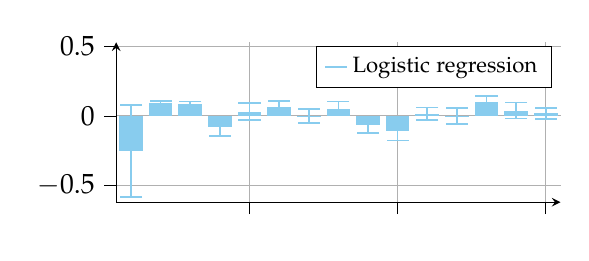
\begin{tikzpicture}

\definecolor{color0}{rgb}{0.533333333333333,0.8,0.933333333333333}

\begin{axis}[
height=1.4222438079424382in,
tick align=outside,
tick pos=left,
width=2.8444876158848764in,
x grid style={white!69.0196078431373!black},
xmajorgrids,
xmin=0.5, xmax=15.5,
xtick style={color=black},
xticklabels={,,},
y grid style={white!69.0196078431373!black},
ymajorgrids,
ymin=-0.623461141126395, ymax=0.530741648814479,
ytick style={color=black},
legend style={font=\footnotesize}
]
\draw[draw=none,fill=color0] (axis cs:0.6,0) rectangle (axis cs:1.4,-0.253461141126395);
\draw[draw=none,fill=color0] (axis cs:1.6,0) rectangle (axis cs:2.4,0.0901171486976447);
\draw[draw=none,fill=color0] (axis cs:2.6,0) rectangle (axis cs:3.4,0.0863947483049856);
\draw[draw=none,fill=color0] (axis cs:3.6,0) rectangle (axis cs:4.4,-0.0772968684905453);
\draw[draw=none,fill=color0] (axis cs:4.6,0) rectangle (axis cs:5.4,0.0300554413526054);
\draw[draw=none,fill=color0] (axis cs:5.6,0) rectangle (axis cs:6.4,0.0644447825923199);
\draw[draw=none,fill=color0] (axis cs:6.6,0) rectangle (axis cs:7.4,0.000906315046421985);
\draw[draw=none,fill=color0] (axis cs:7.6,0) rectangle (axis cs:8.4,0.0527024964515279);
\draw[draw=none,fill=color0] (axis cs:8.6,0) rectangle (axis cs:9.4,-0.0642484568407123);
\draw[draw=none,fill=color0] (axis cs:9.6,0) rectangle (axis cs:10.4,-0.111007430848113);
\draw[draw=none,fill=color0] (axis cs:10.6,0) rectangle (axis cs:11.4,0.0148183210539744);
\draw[draw=none,fill=color0] (axis cs:11.6,0) rectangle (axis cs:12.4,-0.000553836590813862);
\draw[draw=none,fill=color0] (axis cs:12.6,0) rectangle (axis cs:13.4,0.100741648814479);
\draw[draw=none,fill=color0] (axis cs:13.6,0) rectangle (axis cs:14.4,0.0378766308558455);
\draw[draw=none,fill=color0] (axis cs:14.6,0) rectangle (axis cs:15.4,0.0181014244362775);
\path [draw=color0, semithick]
(axis cs:1,-0.587142604409583)
--(axis cs:1,0.0802203221567937);

\path [draw=color0, semithick]
(axis cs:2,0.0731623861401247)
--(axis cs:2,0.107071911255165);

\path [draw=color0, semithick]
(axis cs:3,0.0687951204204073)
--(axis cs:3,0.103994376189564);

\path [draw=color0, semithick]
(axis cs:4,-0.146499644473957)
--(axis cs:4,-0.0080940925071333);

\path [draw=color0, semithick]
(axis cs:5,-0.0313238410576597)
--(axis cs:5,0.0914347237628705);

\path [draw=color0, semithick]
(axis cs:6,0.0198594131562677)
--(axis cs:6,0.109030152028372);

\path [draw=color0, semithick]
(axis cs:7,-0.0499168743976032)
--(axis cs:7,0.0517295044904472);

\path [draw=color0, semithick]
(axis cs:8,0.00179966720486961)
--(axis cs:8,0.103605325698186);

\path [draw=color0, semithick]
(axis cs:9,-0.124803037939885)
--(axis cs:9,-0.00369387574154015);

\path [draw=color0, semithick]
(axis cs:10,-0.178052830807337)
--(axis cs:10,-0.0439620308888901);

\path [draw=color0, semithick]
(axis cs:11,-0.0315422676418746)
--(axis cs:11,0.0611789097498233);

\path [draw=color0, semithick]
(axis cs:12,-0.0592218306178204)
--(axis cs:12,0.0581141574361927);

\path [draw=color0, semithick]
(axis cs:13,0.0576301597775916)
--(axis cs:13,0.143853137851366);

\path [draw=color0, semithick]
(axis cs:14,-0.0196357412360911)
--(axis cs:14,0.0953890029477821);

\path [draw=color0, semithick]
(axis cs:15,-0.0217054681168758)
--(axis cs:15,0.0579083169894307);

\addplot [semithick, color0, mark=-, mark size=4, mark options={solid}, only marks]
table {%
1 -0.587142604409583
2 0.0731623861401247
3 0.0687951204204073
4 -0.146499644473957
5 -0.0313238410576597
6 0.0198594131562677
7 -0.0499168743976032
8 0.00179966720486961
9 -0.124803037939885
10 -0.178052830807337
11 -0.0315422676418746
12 -0.0592218306178204
13 0.0576301597775916
14 -0.0196357412360911
15 -0.0217054681168758
};
\addplot [semithick, color0, mark=-, mark size=4, mark options={solid}, only marks]
table {%
1 0.0802203221567937
2 0.107071911255165
3 0.103994376189564
4 -0.0080940925071333
5 0.0914347237628705
6 0.109030152028372
7 0.0517295044904472
8 0.103605325698186
9 -0.00369387574154015
10 -0.0439620308888901
11 0.0611789097498233
12 0.0581141574361927
13 0.143853137851366
14 0.0953890029477821
15 0.0579083169894307
};
\addlegendimage{semithick, color=color0};
\addlegendentry{Logistic regression};
\end{axis}

\end{tikzpicture}

    \label{fig:03-fi-a}
  \end{subfigure}%
  
  \begin{subfigure}[b]{0.5\textwidth}
    \centering
    % This file was created by tikzplotlib v0.9.8.
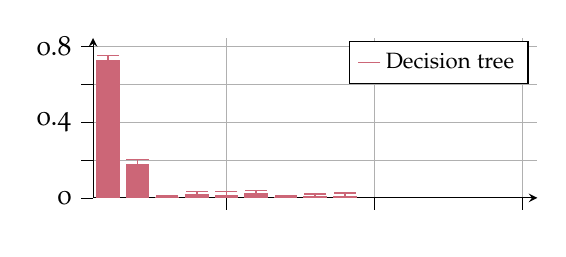
\begin{tikzpicture}

\definecolor{color0}{rgb}{0.8,0.4,0.466666666666667}

\begin{axis}[
height=1.4222438079424382in,
tick align=outside,
tick pos=left,
width=2.8444876158848764in,
x grid style={white!69.0196078431373!black},
xmajorgrids,
xmin=0.5, xmax=15.5,
xtick style={color=black},
xticklabels={,,},
y grid style={white!69.0196078431373!black},
ymajorgrids,
ymin=0, ymax=0.84619547527771,
ytick style={color=black},
yticklabels={,0,, 0.4,,0.8},
legend style={font=\footnotesize}
]
\draw[draw=none,fill=color0] (axis cs:0.6,0) rectangle (axis cs:1.4,0.731619547527771);
\draw[draw=none,fill=color0] (axis cs:1.6,0) rectangle (axis cs:2.4,0.18113983898672);
\draw[draw=none,fill=color0] (axis cs:2.6,0) rectangle (axis cs:3.4,0.00345402728374034);
\draw[draw=none,fill=color0] (axis cs:3.6,0) rectangle (axis cs:4.4,0.0208705310819208);
\draw[draw=none,fill=color0] (axis cs:4.6,0) rectangle (axis cs:5.4,0.0155739365467582);
\draw[draw=none,fill=color0] (axis cs:5.6,0) rectangle (axis cs:6.4,0.0237724911651494);
\draw[draw=none,fill=color0] (axis cs:6.6,0) rectangle (axis cs:7.4,0.003003922613769);
\draw[draw=none,fill=color0] (axis cs:7.6,0) rectangle (axis cs:8.4,0.00923425403456265);
\draw[draw=none,fill=color0] (axis cs:8.6,0) rectangle (axis cs:9.4,0.0113314507596083);
\path [draw=color0, semithick]
(axis cs:1,0.709690218797472)
--(axis cs:1,0.753548876258071);

\path [draw=color0, semithick]
(axis cs:2,0.159795728748012)
--(axis cs:2,0.202483949225428);

\path [draw=color0, semithick]
(axis cs:3,-0.00265218119467417)
--(axis cs:3,0.00956023576215485);

\path [draw=color0, semithick]
(axis cs:4,0.00724021662950192)
--(axis cs:4,0.0345008455343396);

\path [draw=color0, semithick]
(axis cs:5,-0.00216067805943182)
--(axis cs:5,0.0333085511529482);

\path [draw=color0, semithick]
(axis cs:6,0.00816087621620421)
--(axis cs:6,0.0393841061140945);

\path [draw=color0, semithick]
(axis cs:7,-0.00231674240297224)
--(axis cs:7,0.00832458763051024);

\path [draw=color0, semithick]
(axis cs:8,-0.002629967814537)
--(axis cs:8,0.0210984758836623);

\path [draw=color0, semithick]
(axis cs:9,-0.00405574281778054)
--(axis cs:9,0.0267186443369972);

\addplot [semithick, color0, mark=-, mark size=4, mark options={solid}, only marks]
table {%
1 0.709690218797472
2 0.159795728748012
3 -0.00265218119467417
4 0.00724021662950192
5 -0.00216067805943182
6 0.00816087621620421
7 -0.00231674240297224
8 -0.002629967814537
9 -0.00405574281778054
};
\addplot [semithick, color0, mark=-, mark size=4, mark options={solid}, only marks]
table {%
1 0.753548876258071
2 0.202483949225428
3 0.00956023576215485
4 0.0345008455343396
5 0.0333085511529482
6 0.0393841061140945
7 0.00832458763051024
8 0.0210984758836623
9 0.0267186443369972
};
\addlegendimage{semithick, color=color0};
\addlegendentry{Decision tree};
\end{axis}

\end{tikzpicture}

    \label{fig:03-fi-b}
  \end{subfigure}%
  
  \begin{subfigure}[b]{0.5\textwidth}
    \centering
    % This file was created by tikzplotlib v0.9.8.
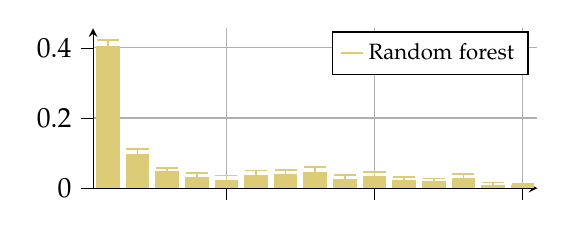
\begin{tikzpicture}

\definecolor{color0}{rgb}{0.866666666666667,0.8,0.466666666666667}

\begin{axis}[
height=1.4222438079424382in,
tick align=outside,
tick pos=left,
width=2.8444876158848764in,
x grid style={white!69.0196078431373!black},
xmajorgrids,
xmin=0.5, xmax=15.5,
xtick style={color=black},
xticklabels={,,},
y grid style={white!69.0196078431373!black},
ymajorgrids,
ymin=0, ymax=0.455941102264594,
ytick style={color=black},
legend style={font=\footnotesize}
]
\draw[draw=none,fill=color0] (axis cs:0.6,0) rectangle (axis cs:1.4,0.405941102264594);
\draw[draw=none,fill=color0] (axis cs:1.6,0) rectangle (axis cs:2.4,0.0980875027579887);
\draw[draw=none,fill=color0] (axis cs:2.6,0) rectangle (axis cs:3.4,0.048776110224331);
\draw[draw=none,fill=color0] (axis cs:3.6,0) rectangle (axis cs:4.4,0.0307695146020032);
\draw[draw=none,fill=color0] (axis cs:4.6,0) rectangle (axis cs:5.4,0.0225284912793522);
\draw[draw=none,fill=color0] (axis cs:5.6,0) rectangle (axis cs:6.4,0.0376912406521808);
\draw[draw=none,fill=color0] (axis cs:6.6,0) rectangle (axis cs:7.4,0.0408639729682783);
\draw[draw=none,fill=color0] (axis cs:7.6,0) rectangle (axis cs:8.4,0.0453356735282065);
\draw[draw=none,fill=color0] (axis cs:8.6,0) rectangle (axis cs:9.4,0.0258685047848363);
\draw[draw=none,fill=color0] (axis cs:9.6,0) rectangle (axis cs:10.4,0.0341199103889856);
\draw[draw=none,fill=color0] (axis cs:10.6,0) rectangle (axis cs:11.4,0.0225669600689547);
\draw[draw=none,fill=color0] (axis cs:11.6,0) rectangle (axis cs:12.4,0.0197271830187896);
\draw[draw=none,fill=color0] (axis cs:12.6,0) rectangle (axis cs:13.4,0.0294260599312947);
\draw[draw=none,fill=color0] (axis cs:13.6,0) rectangle (axis cs:14.4,0.0100732082030255);
\draw[draw=none,fill=color0] (axis cs:14.6,0) rectangle (axis cs:15.4,0.00768012576296064);
\path [draw=color0, semithick]
(axis cs:1,0.38913349982482)
--(axis cs:1,0.422748704704367);

\path [draw=color0, semithick]
(axis cs:2,0.0842715544768568)
--(axis cs:2,0.111903451039121);

\path [draw=color0, semithick]
(axis cs:3,0.0397491095240302)
--(axis cs:3,0.0578031109246318);

\path [draw=color0, semithick]
(axis cs:4,0.0174838367514499)
--(axis cs:4,0.0440551924525565);

\path [draw=color0, semithick]
(axis cs:5,0.00917160744440918)
--(axis cs:5,0.0358853751142952);

\path [draw=color0, semithick]
(axis cs:6,0.0246759311379229)
--(axis cs:6,0.0507065501664387);

\path [draw=color0, semithick]
(axis cs:7,0.0296874637992993)
--(axis cs:7,0.0520404821372574);

\path [draw=color0, semithick]
(axis cs:8,0.0303547427614151)
--(axis cs:8,0.0603166042949978);

\path [draw=color0, semithick]
(axis cs:9,0.0147923986315111)
--(axis cs:9,0.0369446109381616);

\path [draw=color0, semithick]
(axis cs:10,0.0226833594028516)
--(axis cs:10,0.0455564613751197);

\path [draw=color0, semithick]
(axis cs:11,0.0134546981738569)
--(axis cs:11,0.0316792219640525);

\path [draw=color0, semithick]
(axis cs:12,0.0115712020878138)
--(axis cs:12,0.0278831639497654);

\path [draw=color0, semithick]
(axis cs:13,0.0188115961460041)
--(axis cs:13,0.0400405237165853);

\path [draw=color0, semithick]
(axis cs:14,0.00377725683628826)
--(axis cs:14,0.0163691595697627);

\path [draw=color0, semithick]
(axis cs:15,0.00393722295943178)
--(axis cs:15,0.0114230285664895);

\addplot [semithick, color0, mark=-, mark size=4, mark options={solid}, only marks]
table {%
1 0.38913349982482
2 0.0842715544768568
3 0.0397491095240302
4 0.0174838367514499
5 0.00917160744440918
6 0.0246759311379229
7 0.0296874637992993
8 0.0303547427614151
9 0.0147923986315111
10 0.0226833594028516
11 0.0134546981738569
12 0.0115712020878138
13 0.0188115961460041
14 0.00377725683628826
15 0.00393722295943178
};
\addplot [semithick, color0, mark=-, mark size=4, mark options={solid}, only marks]
table {%
1 0.422748704704367
2 0.111903451039121
3 0.0578031109246318
4 0.0440551924525565
5 0.0358853751142952
6 0.0507065501664387
7 0.0520404821372574
8 0.0603166042949978
9 0.0369446109381616
10 0.0455564613751197
11 0.0316792219640525
12 0.0278831639497654
13 0.0400405237165853
14 0.0163691595697627
15 0.0114230285664895
};
\addlegendimage{semithick, color=color0};
\addlegendentry{Random forest};
\end{axis}

\end{tikzpicture}

    \label{fig:03-fi-c}
  \end{subfigure}%
  
  \begin{subfigure}[b]{0.5\textwidth}
    \centering
    % This file was created by tikzplotlib v0.9.8.
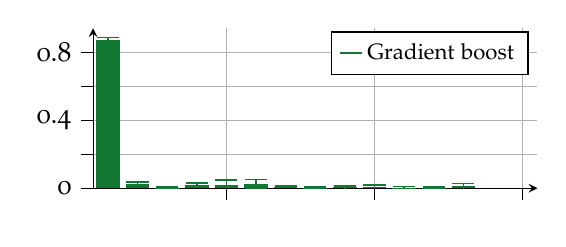
\begin{tikzpicture}

\definecolor{color0}{rgb}{0.0666666666666667,0.466666666666667,0.2}

\begin{axis}[
height=1.4222438079424382in,
tick align=outside,
tick pos=left,
width=2.8444876158848764in,
x grid style={white!69.0196078431373!black},
xmajorgrids,
xmin=0.5, xmax=15.5,
xtick style={color=black},
xticklabels={,,},
y grid style={white!69.0196078431373!black},
ymajorgrids,
ymin=0, ymax=0.941178662009005,
yticklabels={,0,, 0.4,,0.8},
ytick style={color=black},
legend style={font=\footnotesize}
]
\draw[draw=none,fill=color0] (axis cs:0.6,0) rectangle (axis cs:1.4,0.871178662009005);
\draw[draw=none,fill=color0] (axis cs:1.6,0) rectangle (axis cs:2.4,0.0217568511840037);
\draw[draw=none,fill=color0] (axis cs:2.6,0) rectangle (axis cs:3.4,0.00253604996390695);
\draw[draw=none,fill=color0] (axis cs:3.6,0) rectangle (axis cs:4.4,0.0192708196133984);
\draw[draw=none,fill=color0] (axis cs:4.6,0) rectangle (axis cs:5.4,0.0198922275506549);
\draw[draw=none,fill=color0] (axis cs:5.6,0) rectangle (axis cs:6.4,0.0260375424696281);
\draw[draw=none,fill=color0] (axis cs:6.6,0) rectangle (axis cs:7.4,0.0063356815006726);
\draw[draw=none,fill=color0] (axis cs:7.6,0) rectangle (axis cs:8.4,0.00319869517406271);
\draw[draw=none,fill=color0] (axis cs:8.6,0) rectangle (axis cs:9.4,0.00540195176007804);
\draw[draw=none,fill=color0] (axis cs:9.6,0) rectangle (axis cs:10.4,0.00695771640251456);
\draw[draw=none,fill=color0] (axis cs:10.6,0) rectangle (axis cs:11.4,0.00312270971606427);
\draw[draw=none,fill=color0] (axis cs:11.6,0) rectangle (axis cs:12.4,0.0030932299465922);
\draw[draw=none,fill=color0] (axis cs:12.6,0) rectangle (axis cs:13.4,0.0112178627094187);
\path [draw=color0, semithick]
(axis cs:1,0.854956014167526)
--(axis cs:1,0.887401309850484);

\path [draw=color0, semithick]
(axis cs:2,0.00907965200713417)
--(axis cs:2,0.0344340503608733);

\path [draw=color0, semithick]
(axis cs:3,-0.000182654889842383)
--(axis cs:3,0.00525475481765629);

\path [draw=color0, semithick]
(axis cs:4,0.00923661909617688)
--(axis cs:4,0.0293050201306199);

\path [draw=color0, semithick]
(axis cs:5,-0.00820788248180509)
--(axis cs:5,0.0479923375831149);

\path [draw=color0, semithick]
(axis cs:6,0.00143690786973603)
--(axis cs:6,0.0506381770695201);

\path [draw=color0, semithick]
(axis cs:7,-0.00149882818592621)
--(axis cs:7,0.0141701911872714);

\path [draw=color0, semithick]
(axis cs:8,-0.00213482608794717)
--(axis cs:8,0.00853221643607259);

\path [draw=color0, semithick]
(axis cs:9,-0.00260933890414728)
--(axis cs:9,0.0134132424243034);

\path [draw=color0, semithick]
(axis cs:10,-0.0038254976017747)
--(axis cs:10,0.0177409304068038);

\path [draw=color0, semithick]
(axis cs:11,-0.0044786262895489)
--(axis cs:11,0.0107240457216774);

\path [draw=color0, semithick]
(axis cs:12,-0.000395131606741384)
--(axis cs:12,0.00658159149992578);

\path [draw=color0, semithick]
(axis cs:13,-0.00413997684116445)
--(axis cs:13,0.0265757022600018);

\addplot [semithick, color0, mark=-, mark size=4, mark options={solid}, only marks]
table {%
1 0.854956014167526
2 0.00907965200713417
3 -0.000182654889842383
4 0.00923661909617688
5 -0.00820788248180509
6 0.00143690786973603
7 -0.00149882818592621
8 -0.00213482608794717
9 -0.00260933890414728
10 -0.0038254976017747
11 -0.0044786262895489
12 -0.000395131606741384
13 -0.00413997684116445
};
\addplot [semithick, color0, mark=-, mark size=4, mark options={solid}, only marks]
table {%
1 0.887401309850484
2 0.0344340503608733
3 0.00525475481765629
4 0.0293050201306199
5 0.0479923375831149
6 0.0506381770695201
7 0.0141701911872714
8 0.00853221643607259
9 0.0134132424243034
10 0.0177409304068038
11 0.0107240457216774
12 0.00658159149992578
13 0.0265757022600018
};
\addlegendimage{semithick, color=color0};
\addlegendentry{Gradient boost};
\end{axis}

\end{tikzpicture}

    \label{fig:03-fi-d}
  \end{subfigure}%
  
  \begin{subfigure}[b]{0.5\textwidth}
    \centering
    % This file was created by tikzplotlib v0.9.8.
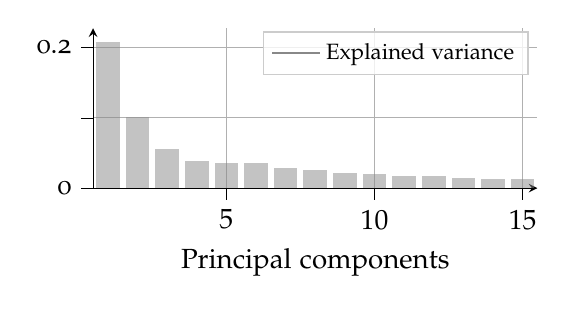
\begin{tikzpicture}

\begin{axis}[
height=1.4222438079424382in,
legend style={fill opacity=0.8, draw opacity=1, text opacity=1, draw=white!80!black},
tick align=outside,
tick pos=left,
width=2.8444876158848764in,
x grid style={white!69.0196078431373!black},
xmajorgrids,
xmin=0.5, xmax=15.5,
xlabel={Principal components},
xtick style={color=black},
y grid style={white!69.0196078431373!black},
ymajorgrids,
ymin=0, ymax=0.227659111193136,
ytick style={color=black},
yticklabels={,0,, 0.2},
legend style={font=\footnotesize}
]
\draw[draw=none,fill=white!53.3333333333333!black,fill opacity=0.5] (axis cs:0.6,0) rectangle (axis cs:1.4,0.207659111193136);
\draw[draw=none,fill=white!53.3333333333333!black,fill opacity=0.5] (axis cs:1.6,0) rectangle (axis cs:2.4,0.100931286761405);
\draw[draw=none,fill=white!53.3333333333333!black,fill opacity=0.5] (axis cs:2.6,0) rectangle (axis cs:3.4,0.0552189869141694);
\draw[draw=none,fill=white!53.3333333333333!black,fill opacity=0.5] (axis cs:3.6,0) rectangle (axis cs:4.4,0.0393144279067069);
\draw[draw=none,fill=white!53.3333333333333!black,fill opacity=0.5] (axis cs:4.6,0) rectangle (axis cs:5.4,0.0359175173728584);
\draw[draw=none,fill=white!53.3333333333333!black,fill opacity=0.5] (axis cs:5.6,0) rectangle (axis cs:6.4,0.0352100230844184);
\draw[draw=none,fill=white!53.3333333333333!black,fill opacity=0.5] (axis cs:6.6,0) rectangle (axis cs:7.4,0.0281116402524651);
\draw[draw=none,fill=white!53.3333333333333!black,fill opacity=0.5] (axis cs:7.6,0) rectangle (axis cs:8.4,0.0255858301182614);
\draw[draw=none,fill=white!53.3333333333333!black,fill opacity=0.5] (axis cs:8.6,0) rectangle (axis cs:9.4,0.020895147833239);
\draw[draw=none,fill=white!53.3333333333333!black,fill opacity=0.5] (axis cs:9.6,0) rectangle (axis cs:10.4,0.020208986578298);
\draw[draw=none,fill=white!53.3333333333333!black,fill opacity=0.5] (axis cs:10.6,0) rectangle (axis cs:11.4,0.0173851755021279);
\draw[draw=none,fill=white!53.3333333333333!black,fill opacity=0.5] (axis cs:11.6,0) rectangle (axis cs:12.4,0.0170402398481309);
\draw[draw=none,fill=white!53.3333333333333!black,fill opacity=0.5] (axis cs:12.6,0) rectangle (axis cs:13.4,0.0150421767580223);
\draw[draw=none,fill=white!53.3333333333333!black,fill opacity=0.5] (axis cs:13.6,0) rectangle (axis cs:14.4,0.0135123051552189);
\draw[draw=none,fill=white!53.3333333333333!black,fill opacity=0.5] (axis cs:14.6,0) rectangle (axis cs:15.4,0.0123812036773514);
\draw[draw=none,fill=white!53.3333333333333!black,fill opacity=0.5] (axis cs:15.6,0) rectangle (axis cs:16.4,0.0121461292946794);
\draw[draw=none,fill=white!53.3333333333333!black,fill opacity=0.5] (axis cs:16.6,0) rectangle (axis cs:17.4,0.0113049221584044);
\draw[draw=none,fill=white!53.3333333333333!black,fill opacity=0.5] (axis cs:17.6,0) rectangle (axis cs:18.4,0.0105679286164572);
\draw[draw=none,fill=white!53.3333333333333!black,fill opacity=0.5] (axis cs:18.6,0) rectangle (axis cs:19.4,0.0099240637848415);
\draw[draw=none,fill=white!53.3333333333333!black,fill opacity=0.5] (axis cs:19.6,0) rectangle (axis cs:20.4,0.00947939547970391);
\draw[draw=none,fill=white!53.3333333333333!black,fill opacity=0.5] (axis cs:20.6,0) rectangle (axis cs:21.4,0.00880748003307345);
\draw[draw=none,fill=white!53.3333333333333!black,fill opacity=0.5] (axis cs:21.6,0) rectangle (axis cs:22.4,0.00854299753930025);
\draw[draw=none,fill=white!53.3333333333333!black,fill opacity=0.5] (axis cs:22.6,0) rectangle (axis cs:23.4,0.00819923337711622);
\draw[draw=none,fill=white!53.3333333333333!black,fill opacity=0.5] (axis cs:23.6,0) rectangle (axis cs:24.4,0.00783441956089457);
\draw[draw=none,fill=white!53.3333333333333!black,fill opacity=0.5] (axis cs:24.6,0) rectangle (axis cs:25.4,0.00725436756435554);
\draw[draw=none,fill=white!53.3333333333333!black,fill opacity=0.5] (axis cs:25.6,0) rectangle (axis cs:26.4,0.00706748361834891);
\draw[draw=none,fill=white!53.3333333333333!black,fill opacity=0.5] (axis cs:26.6,0) rectangle (axis cs:27.4,0.0067946334120975);
\draw[draw=none,fill=white!53.3333333333333!black,fill opacity=0.5] (axis cs:27.6,0) rectangle (axis cs:28.4,0.00649269621923748);
\draw[draw=none,fill=white!53.3333333333333!black,fill opacity=0.5] (axis cs:28.6,0) rectangle (axis cs:29.4,0.00631012021109268);
\draw[draw=none,fill=white!53.3333333333333!black,fill opacity=0.5] (axis cs:29.6,0) rectangle (axis cs:30.4,0.0059935965924482);
\draw[draw=none,fill=white!53.3333333333333!black,fill opacity=0.5] (axis cs:30.6,0) rectangle (axis cs:31.4,0.00591276082294336);
\draw[draw=none,fill=white!53.3333333333333!black,fill opacity=0.5] (axis cs:31.6,0) rectangle (axis cs:32.4,0.00563442172532614);
\draw[draw=none,fill=white!53.3333333333333!black,fill opacity=0.5] (axis cs:32.6,0) rectangle (axis cs:33.4,0.00539612814948874);
\draw[draw=none,fill=white!53.3333333333333!black,fill opacity=0.5] (axis cs:33.6,0) rectangle (axis cs:34.4,0.00529456870611715);
\draw[draw=none,fill=white!53.3333333333333!black,fill opacity=0.5] (axis cs:34.6,0) rectangle (axis cs:35.4,0.0052012922431412);
\draw[draw=none,fill=white!53.3333333333333!black,fill opacity=0.5] (axis cs:35.6,0) rectangle (axis cs:36.4,0.00496741617032561);
\draw[draw=none,fill=white!53.3333333333333!black,fill opacity=0.5] (axis cs:36.6,0) rectangle (axis cs:37.4,0.00483584771153227);
\draw[draw=none,fill=white!53.3333333333333!black,fill opacity=0.5] (axis cs:37.6,0) rectangle (axis cs:38.4,0.00475069774706768);
\draw[draw=none,fill=white!53.3333333333333!black,fill opacity=0.5] (axis cs:38.6,0) rectangle (axis cs:39.4,0.00453755427803973);
\draw[draw=none,fill=white!53.3333333333333!black,fill opacity=0.5] (axis cs:39.6,0) rectangle (axis cs:40.4,0.00431289524873035);
\draw[draw=none,fill=white!53.3333333333333!black,fill opacity=0.5] (axis cs:40.6,0) rectangle (axis cs:41.4,0.00413291864955501);
\draw[draw=none,fill=white!53.3333333333333!black,fill opacity=0.5] (axis cs:41.6,0) rectangle (axis cs:42.4,0.00404009691245206);
\draw[draw=none,fill=white!53.3333333333333!black,fill opacity=0.5] (axis cs:42.6,0) rectangle (axis cs:43.4,0.00384707175639724);
\draw[draw=none,fill=white!53.3333333333333!black,fill opacity=0.5] (axis cs:43.6,0) rectangle (axis cs:44.4,0.00370794252319461);
\draw[draw=none,fill=white!53.3333333333333!black,fill opacity=0.5] (axis cs:44.6,0) rectangle (axis cs:45.4,0.00360347785161737);
\draw[draw=none,fill=white!53.3333333333333!black,fill opacity=0.5] (axis cs:45.6,0) rectangle (axis cs:46.4,0.00350293803678438);
\draw[draw=none,fill=white!53.3333333333333!black,fill opacity=0.5] (axis cs:46.6,0) rectangle (axis cs:47.4,0.00335377406642866);
\draw[draw=none,fill=white!53.3333333333333!black,fill opacity=0.5] (axis cs:47.6,0) rectangle (axis cs:48.4,0.00332782254644005);
\draw[draw=none,fill=white!53.3333333333333!black,fill opacity=0.5] (axis cs:48.6,0) rectangle (axis cs:49.4,0.00325065460225723);
\draw[draw=none,fill=white!53.3333333333333!black,fill opacity=0.5] (axis cs:49.6,0) rectangle (axis cs:50.4,0.00312401268859448);
\draw[draw=none,fill=white!53.3333333333333!black,fill opacity=0.5] (axis cs:50.6,0) rectangle (axis cs:51.4,0.00307409451814868);
\draw[draw=none,fill=white!53.3333333333333!black,fill opacity=0.5] (axis cs:51.6,0) rectangle (axis cs:52.4,0.00295493366839609);
\draw[draw=none,fill=white!53.3333333333333!black,fill opacity=0.5] (axis cs:52.6,0) rectangle (axis cs:53.4,0.00283452933734321);
\draw[draw=none,fill=white!53.3333333333333!black,fill opacity=0.5] (axis cs:53.6,0) rectangle (axis cs:54.4,0.00281415629292076);
\draw[draw=none,fill=white!53.3333333333333!black,fill opacity=0.5] (axis cs:54.6,0) rectangle (axis cs:55.4,0.00277164449537654);
\draw[draw=none,fill=white!53.3333333333333!black,fill opacity=0.5] (axis cs:55.6,0) rectangle (axis cs:56.4,0.0027301380386249);
\draw[draw=none,fill=white!53.3333333333333!black,fill opacity=0.5] (axis cs:56.6,0) rectangle (axis cs:57.4,0.00269085035745271);
\draw[draw=none,fill=white!53.3333333333333!black,fill opacity=0.5] (axis cs:57.6,0) rectangle (axis cs:58.4,0.00256884319342844);
\draw[draw=none,fill=white!53.3333333333333!black,fill opacity=0.5] (axis cs:58.6,0) rectangle (axis cs:59.4,0.00252762617436217);
\draw[draw=none,fill=white!53.3333333333333!black,fill opacity=0.5] (axis cs:59.6,0) rectangle (axis cs:60.4,0.00237101574205109);
\draw[draw=none,fill=white!53.3333333333333!black,fill opacity=0.5] (axis cs:60.6,0) rectangle (axis cs:61.4,0.0023429271914207);
\draw[draw=none,fill=white!53.3333333333333!black,fill opacity=0.5] (axis cs:61.6,0) rectangle (axis cs:62.4,0.00230359137012767);
\draw[draw=none,fill=white!53.3333333333333!black,fill opacity=0.5] (axis cs:62.6,0) rectangle (axis cs:63.4,0.00221364734281885);
\draw[draw=none,fill=white!53.3333333333333!black,fill opacity=0.5] (axis cs:63.6,0) rectangle (axis cs:64.4,0.0021462360088001);
\draw[draw=none,fill=white!53.3333333333333!black,fill opacity=0.5] (axis cs:64.6,0) rectangle (axis cs:65.4,0.00211833683255068);
\draw[draw=none,fill=white!53.3333333333333!black,fill opacity=0.5] (axis cs:65.6,0) rectangle (axis cs:66.4,0.00205592806762017);
\draw[draw=none,fill=white!53.3333333333333!black,fill opacity=0.5] (axis cs:66.6,0) rectangle (axis cs:67.4,0.00203631661765791);
\draw[draw=none,fill=white!53.3333333333333!black,fill opacity=0.5] (axis cs:67.6,0) rectangle (axis cs:68.4,0.00200913992503488);
\draw[draw=none,fill=white!53.3333333333333!black,fill opacity=0.5] (axis cs:68.6,0) rectangle (axis cs:69.4,0.00198860732256562);
\draw[draw=none,fill=white!53.3333333333333!black,fill opacity=0.5] (axis cs:69.6,0) rectangle (axis cs:70.4,0.00191877504746405);
\draw[draw=none,fill=white!53.3333333333333!black,fill opacity=0.5] (axis cs:70.6,0) rectangle (axis cs:71.4,0.00183983787651402);
\draw[draw=none,fill=white!53.3333333333333!black,fill opacity=0.5] (axis cs:71.6,0) rectangle (axis cs:72.4,0.00178967267072127);
\draw[draw=none,fill=white!53.3333333333333!black,fill opacity=0.5] (axis cs:72.6,0) rectangle (axis cs:73.4,0.00176113054018146);
\draw[draw=none,fill=white!53.3333333333333!black,fill opacity=0.5] (axis cs:73.6,0) rectangle (axis cs:74.4,0.00175587755437847);
\draw[draw=none,fill=white!53.3333333333333!black,fill opacity=0.5] (axis cs:74.6,0) rectangle (axis cs:75.4,0.00166568926296783);
\draw[draw=none,fill=white!53.3333333333333!black,fill opacity=0.5] (axis cs:75.6,0) rectangle (axis cs:76.4,0.00164865674220492);
\draw[draw=none,fill=white!53.3333333333333!black,fill opacity=0.5] (axis cs:76.6,0) rectangle (axis cs:77.4,0.00163963642273892);
\draw[draw=none,fill=white!53.3333333333333!black,fill opacity=0.5] (axis cs:77.6,0) rectangle (axis cs:78.4,0.00152246485297179);
\draw[draw=none,fill=white!53.3333333333333!black,fill opacity=0.5] (axis cs:78.6,0) rectangle (axis cs:79.4,0.00150671318108692);
\draw[draw=none,fill=white!53.3333333333333!black,fill opacity=0.5] (axis cs:79.6,0) rectangle (axis cs:80.4,0.00146762230969936);
\draw[draw=none,fill=white!53.3333333333333!black,fill opacity=0.5] (axis cs:80.6,0) rectangle (axis cs:81.4,0.00144254604987905);
\draw[draw=none,fill=white!53.3333333333333!black,fill opacity=0.5] (axis cs:81.6,0) rectangle (axis cs:82.4,0.00142852516970499);
\draw[draw=none,fill=white!53.3333333333333!black,fill opacity=0.5] (axis cs:82.6,0) rectangle (axis cs:83.4,0.00140797817653715);
\draw[draw=none,fill=white!53.3333333333333!black,fill opacity=0.5] (axis cs:83.6,0) rectangle (axis cs:84.4,0.00137907370730369);
\draw[draw=none,fill=white!53.3333333333333!black,fill opacity=0.5] (axis cs:84.6,0) rectangle (axis cs:85.4,0.00137189411391102);
\draw[draw=none,fill=white!53.3333333333333!black,fill opacity=0.5] (axis cs:85.6,0) rectangle (axis cs:86.4,0.00134894755604915);
\draw[draw=none,fill=white!53.3333333333333!black,fill opacity=0.5] (axis cs:86.6,0) rectangle (axis cs:87.4,0.00131887269241828);
\draw[draw=none,fill=white!53.3333333333333!black,fill opacity=0.5] (axis cs:87.6,0) rectangle (axis cs:88.4,0.00125161529911504);
\draw[draw=none,fill=white!53.3333333333333!black,fill opacity=0.5] (axis cs:88.6,0) rectangle (axis cs:89.4,0.00123038981331776);
\draw[draw=none,fill=white!53.3333333333333!black,fill opacity=0.5] (axis cs:89.6,0) rectangle (axis cs:90.4,0.00120293547721247);
\draw[draw=none,fill=white!53.3333333333333!black,fill opacity=0.5] (axis cs:90.6,0) rectangle (axis cs:91.4,0.00118929296627723);
\draw[draw=none,fill=white!53.3333333333333!black,fill opacity=0.5] (axis cs:91.6,0) rectangle (axis cs:92.4,0.00115421686183217);
\draw[draw=none,fill=white!53.3333333333333!black,fill opacity=0.5] (axis cs:92.6,0) rectangle (axis cs:93.4,0.00113288923394035);
\draw[draw=none,fill=white!53.3333333333333!black,fill opacity=0.5] (axis cs:93.6,0) rectangle (axis cs:94.4,0.00108899958168978);
\draw[draw=none,fill=white!53.3333333333333!black,fill opacity=0.5] (axis cs:94.6,0) rectangle (axis cs:95.4,0.00107268732150737);
\draw[draw=none,fill=white!53.3333333333333!black,fill opacity=0.5] (axis cs:95.6,0) rectangle (axis cs:96.4,0.00104142782755626);
\draw[draw=none,fill=white!53.3333333333333!black,fill opacity=0.5] (axis cs:96.6,0) rectangle (axis cs:97.4,0.00101906762512476);
\draw[draw=none,fill=white!53.3333333333333!black,fill opacity=0.5] (axis cs:97.6,0) rectangle (axis cs:98.4,0.00101077830297021);
\draw[draw=none,fill=white!53.3333333333333!black,fill opacity=0.5] (axis cs:98.6,0) rectangle (axis cs:99.4,0.000989640667068959);
\draw[draw=none,fill=white!53.3333333333333!black,fill opacity=0.5] (axis cs:99.6,0) rectangle (axis cs:100.4,0.000984439118691105);
\draw[draw=none,fill=white!53.3333333333333!black,fill opacity=0.5] (axis cs:100.6,0) rectangle (axis cs:101.4,0.000960734989790538);
\draw[draw=none,fill=white!53.3333333333333!black,fill opacity=0.5] (axis cs:101.6,0) rectangle (axis cs:102.4,0.000941461336335633);
\draw[draw=none,fill=white!53.3333333333333!black,fill opacity=0.5] (axis cs:102.6,0) rectangle (axis cs:103.4,0.000928355012563315);
\draw[draw=none,fill=white!53.3333333333333!black,fill opacity=0.5] (axis cs:103.6,0) rectangle (axis cs:104.4,0.000913315342059004);
\draw[draw=none,fill=white!53.3333333333333!black,fill opacity=0.5] (axis cs:104.6,0) rectangle (axis cs:105.4,0.000897708116603778);
\draw[draw=none,fill=white!53.3333333333333!black,fill opacity=0.5] (axis cs:105.6,0) rectangle (axis cs:106.4,0.000874661763686027);
\draw[draw=none,fill=white!53.3333333333333!black,fill opacity=0.5] (axis cs:106.6,0) rectangle (axis cs:107.4,0.000854349918034593);
\draw[draw=none,fill=white!53.3333333333333!black,fill opacity=0.5] (axis cs:107.6,0) rectangle (axis cs:108.4,0.000841201883286582);
\draw[draw=none,fill=white!53.3333333333333!black,fill opacity=0.5] (axis cs:108.6,0) rectangle (axis cs:109.4,0.000819094760963474);
\addlegendimage{semithick, color=white!53.3333333333333!black};
\addlegendentry{Explained variance};
\end{axis}

\end{tikzpicture}

    \label{fig:03-fi-e}
  \end{subfigure}%
  
  \caption{Visualization of different parameters for the $15$ most principal components ranked in descending order by the explained variance for the empirical approach. The panels show the logistic regression coefficients, decision trees feature importance, random forests feature importance, gradient boosting feature importance, and explained variance that is retained by including each of the eigenvectors. }
  \label{fig:03-fi}
\end{figure}

Lastly, gradient boosting performs optimally at $13$ principal components with a mean F$1$-score of $0.96$. The relevant hyperparameters were the regularization term for logistic regression, which was set to $0.021$, and the maximum number of iterations at $400$. The decision trees uses a maximum depth of $6$, where larger values increased the training accuracy but not any other metric. The maximum depth for  random forests was set to $6$. For gradient boosting, which uses a weak learner, the depth of the trees was set to  $4$. 

%OH: Commented out the three next paragraphs, since this is mentioned in main text.
%The empirical approach differs in many aspects from the Ferrenti and extended Ferrenti approaches. Firstly, we find that the number of principal components necessary to obtain $95 \ \%$ variance is reduced to $103$ components, which is $41$ and $56$ less than the Ferrenti and extended Ferrenti approach, respectively. Thus, the variance of the training set is found to be described with fewer principal components, indicating a simpler model.   

%Secondly, we find that the first principal component is by far the most important feature for all models, as visualized in Figure~\ref{fig:03-fi}. This is part of the reason why we experience a large accuracy for only a single feature, as seen in Figure~\ref{fig:03-pca}. The first principal component's corresponding features are challenging to explain due to small variations of values, but we see it including 
%However, it differs when it comes to which top features the first principal component describes, which includes 
%bond orientational parameters, coordination numbers, and the radial distribution function of a compound's crystal system.

%Thirdly, the empirical approach differs in how much explained variation is retained by the first component, which is $21 \ \%$, while it is $14 \ \%$ for the Ferrenti approach and $11 \ \%$ for the extended Ferrenti approach. We find the difference striking considering that the approaches share the same ultimate goal, but where the training sets apparently exhibit large and significant variations. 


\begin{figure}[t]
    \centering
    (a) Ferrenti approach
    \\
    \begin{forest}
        for tree={l sep=1em, s sep=1em, anchor=center, inner sep=0.3em, fill=red!50, circle}
        [$23623$ compounds, node box, alias=bagging, above=1em
        [Logistic regression,node box,alias=a1
          [$11243$]
          [$12380$,fill=green!50,edge label={node[above=1ex,green arrow]{}}
          ]
        ]
        [Decision trees,node box,alias=a1
          [$12308$]
          [$11315$,fill=green!50,edge label={node[above=1ex,green arrow]{}}
          ]
        ]
        [Random forests,node box,alias=a1
          [$9345$]
          [$14278$,fill=green!50,edge label={node[above=1ex,green arrow]{}}
          ]
        ]
        [Gradient boosting,node box,alias=a1
          [$11835$]
          [$11788$,fill=green!50,edge label={node[above=1ex,green arrow]{}}
          ]
        ]
        ]
    \end{forest}
%\vspace*{-95mm}
    \\
    (b) Augmented Ferrenti approach 
    \\
\begin{forest}
    for tree={l sep=1em, s sep=1em, anchor=center, inner sep=0.3em, fill=red!50, circle}
    [$22550$ compounds, node box, alias=bagging, above=1em
    [Logistic regression,node box,alias=a1
      [$7557$]
      [$14993$,fill=green!50,edge label={node[above=1ex,green arrow]{}}
      ]
    ]
    [Decision trees,node box,alias=a1
      [$8143$]
      [$14407$,fill=green!50,edge label={node[above=1ex,green arrow]{}}
      ]
    ]
    [Random forests,node box,alias=a1
      [$7199$]
      [$15351$,fill=green!50,edge label={node[above=1ex,green arrow]{}}
      ]
    ]
    [Gradient boosting,node box,alias=a1
      [$8762$]
      [$13788$,fill=green!50,edge label={node[above=1ex,green arrow]{}}
      ]
    ]
    ]
  \end{forest}
%\vspace*{20mm}
    \\
    (c) Intuitive approach
    \\
 \begin{forest}
    for tree={l sep=1em, s sep=1em, anchor=center, inner sep=0.3em, fill=red!50, circle}
    [$24544$ compounds, node box, alias=bagging, above=1em
    [Logistic regression,node box,alias=a1
      [$23702$]
      [$842$,fill=green!50,edge label={node[above=1ex,green arrow]{}}
      ]
    ]
    [Decision trees,node box,alias=a1
      [$23347$]
      [$1197$,fill=green!50,edge label={node[above=1ex,green arrow]{}}
      ]
    ]
    [Random forests,node box,alias=a1
      [$24001$]
      [$543$,fill=green!50,edge label={node[above=1ex,green arrow]{}}
      ]
    ]
    [Gradient boosting,node box,alias=a1
      [$23948$]
      [$596$,fill=green!50,edge label={node[above=1ex,green arrow]{}}
      ]
    ]
    ]
  \end{forest}
%\vspace*{-95mm}
\caption{Visualization of the predicted material candidates from the (a) Ferrenti, (b) augmented Ferrenti and (c) intuitive approaches. Green and red nodes represent suitable and unsuitable candidates, respectively. }
\label{fig:predictions}
\end{figure}



\section*{Supplementary results} 

\subsection*{Prediction statistics}

Figure~\ref{fig:predictions} provides a visualization of the number of predicted material candidates from the (a) Ferrenti, (b) extended Ferrenti and (c) empirical approaches. Suitable and unsuitable candidates are marked in green and red, respectively. We observe that the number of predicted suitable candidates is similar for the Ferrenti and extended Ferrenti approaches, albeit higher in the case of the latter, for all four ML methods, while the empirical approach results in a substantially narrower selection of contender materials. Note that the confidence threshold was set to $0.5$ in this case. 

For the Ferrenti approach, logistic regression finds a total of $12.380$ suitable candidates, while decision trees is the most conservative with $11.315$. Random forests has the most optimistic estimate with $14.278$, while gradient boosting finds $11.835$ suitable candidates. The four ML methods agree on $6804$ suitable candidates,  however, many of the materials are predicted with a confidence similar to that of a coin-flip.
If we were to raise the minimum bar of a prediction to  
%$0.7$, the four methods would only agree on $3000$ suitable candidates
$0.75$, the four methods would only agree on $1784$ suitable candidates. 

The perhaps more liberal extended Ferrenti approach yields the largest number of predicted candidates with $14.993$, $14.407$, $15.351$ and $13.788$ for logistic regression, decision trees, random forests, and gradient boosting, respectively. Due to the less stringent restrictions compared to the Ferrenti approach, we find a large number ($9227$) of entries that the four ML methods  agree on.

The four ML methods predict radically fewer suitable candidates for the empirical approach as compared to the two former approaches, where only $842$, $1197$, $543$, and $596$ materials are predicted as suitable by logistic regression, decision trees, random forests, and gradient boosting, respectively. The large majority of the unsuitable candidates are predicted with high probability except for random forests due to the ensemble of trees. All methods, however, agree on $214$ suitable candidates above a $0.5$ threshold limit.  

\subsection*{Predicted materials}

Table~\ref{tab:03-probability-candidates} displays the $66$ predicted candidate materials that all four machine learning methods, using the training and test sets derived in the empirical approach, agreed on with a confidence cut-off set to $0.75$. All band gaps are taken from the Materials Project database as calculated using DFT and the PBE functional. Note that materials can appear several times in the list due  to  different  structures of the same composition. The  list  contains $5$ elementary (unary), $46$ binary and  $15$ ternary compounds. 

\begin{center}
\begin{longtable}{M{3.5cm} M{6.5cm} M{2.0cm}}
\caption{The $66$ predicted candidates that all models in the intuitive approach agreed on to a cut-off of $0.75$. All band gaps were taken from the Materials Project (MP) database, and materials can appear several times in the list due to different structures. The list contains $5$ elementary (unary), $46$ binary and $15$ ternary compounds.}
\label{tab:03-probability-candidates}  
\\ \hline
Compound formula & MP ID & Band gap from MP (eV) \\
\hline
  Ge & mp-137 & 0.87\\
  CdTe & mp-406 & 1.22\\
  HgSe & mp-820 & 0.12\\
  GeTe & mp-938 & 0.82\\
  MgTe & mp-1039 & 2.36\\
  CdSe & mp-1070 & 0.55\\
  GaSb & mp-1156 & 0.36\\
  BP & mp-1479 & 1.46\\
  MoSe$_2$ & mp-1634 & 1.41\\
  BN & mp-1639 & 4.64\\
  YbTe & mp-1779 & 1.52\\
  SnS & mp-1876 & 0.95\\
  SnTe & mp-1883 & 0.66\\
  GeTe & mp-2612 & 0.61\\
  AlSb & mp-2624 & 1.26\\
  CdSe & mp-2691 & 0.50\\
  SnSe & mp-2693 & 0.82\\
  CdSnAs$_2$ & mp-3829 & 0.30\\
  GaCuTe$_2$ & mp-3839 & 0.55\\
  ZnGeAs$_2$ & mp-4008 & 0.56\\
  ZnGeP$_2$ & mp-4524 & 1.20\\
  GaAgTe$_2$ & mp-4899 & 0.19\\
  CdSnP$_2$ & mp-5213 & 0.67\\
  GaCuS$_2$ & mp-5238 & 0.70\\
  SnS & mp-10013 & 0.23\\
  BAs & mp-10044 & 1.25\\
  GeSe & mp-10759 & 0.44\\
  MgSe & mp-10760 & 1.97\\
  CdTe & mp-12779 & 0.61\\
  MgSe & mp-13031 & 2.54\\
  MgTe & mp-13033 & 2.31\\
  TePb & mp-19717 & 1.05\\
  InAs & mp-20305 & 0.30\\
  InP & mp-20351 & 0.46\\
  InAgSe$_2$ & mp-20554 & 0.36\\
  InN & mp-22205 & 0.47\\
  AgI & mp-22894 & 1.39\\
  CuI & mp-22895 & 1.17\\
  CuBr & mp-22913 & 0.48\\
  CuCl & mp-22914 & 0.80\\
  AgI & mp-22919 & 1.00\\
  AgI & mp-22925 & 1.72\\
  Br & mp-23154 & 1.32\\
  TlI & mp-23197 & 2.25\\
  AgBr & mp-23231 & 0.79\\
  BC$_2$N & mp-30148 & 2.10\\
  CuI & mp-569346 & 1.21\\
  Hg & mp-569360 & 0.22\\
  Ga$_2$Os & mp-570875 & 0.66\\
  BC$_2$N & mp-629458 & 1.84\\
  InP & mp-966800 & 0.51\\
  GeC & mp-1002164 & 1.84\\
  TlP & mp-1007776 & 0.12\\
  BC$_2$N & mp-1008523 & 1.64\\
  BP & mp-1008559 & 1.07\\
  OsC & mp-1009540 & 0.17\\
  SiSn & mp-1009813 & 0.41\\
  ZnCdSe$_2$ & mp-1017534 & 1.85\\
  MgSe & mp-1018040 & 2.57\\
  AlSb & mp-1018100 & 0.91\\
  AlBi & mp-1018132 & 0.30\\
  Ge & mp-1067619 & 0.791\\
  Ga$_2$Ru & mp-1072429 & 0.12\\
  ZnCd$_3$Se$_4$ & mp-1078597 & 1.72\\
  BC$_2$N & mp-1079201 & 1.17\\
  Ge & mp-1198022 & 0.67\\
  \hline
\end{longtable}
\end{center}


Table~\ref{tab:04-probability-candidates} displays the $47$ predicted candidates that all four machine learning methods and all three approaches (Ferrenti, extended Ferrenti and empirical) agreed on (to a $0.5$ cut-off value).    
The list contains $8$ elemental, $29$ binary, and $10$ tertiary compounds.

\begin{center}
\begin{longtable}{M{3.5cm} M{6.5cm} M{2.0cm}}
\caption{A table displaying the $46$? predicted candidates that all models and all approaches agree on.}
\label{tab:03-probability-candidates}  
\hline
Compound formula & MP ID & Band gap from MP (eV) \\
\hline
  P & mp-157 & 7.47\\
  SiRu & mp-189 & 0.63\\
  BN & mp-344 & 0.41\\
  HgSe & mp-820 & 3.96\\
  FeSi & mp-871 & 2.06\\
  MgTe & mp-1039 & 6.62\\
  CdSe & mp-1070 & 3.91\\
  BP & mp-1479 & 2.89\\
  CdSe & mp-2691 & 2.40\\
  ZnSiAs$_2$ & mp-3595 & 1.57\\
  ZnGeAs$_2$ & mp-4008 & 1.52\\
  CdSnP$_2$ & mp-5213 & 0.95\\
  Si$_2$Mo & mp-8938 & 0.66\\
  BAs & mp-10044 & 0.61\\
  GeSe & mp-10759 & 1.26\\
  N$_2$ & mp-12103 & 0.50\\
  BeSiN$_2$ & mp-15704 & 0.82\\
  InP & mp-20351 & 0.30\\
  InN & mp-22205 & 0.55\\
  AgCl & mp-22922 & 0.56\\
  I & mp-23153 & 1.20\\
  Br & mp-23154 & 0.19\\
  TlI & mp-23197 & 0.67\\
  AgBr & mp-23231 & 0.70\\
  H$_2$ & mp-23907 & 0.23\\
  Ge$_3$As$_4$ & mp-569600 & 1.25\\
  TlCl & mp-569639 & 0.44\\
  Sn$_3$As$_4$ & mp-570377 & 1.97\\
  H$_2$ & mp-634659 & 0.61\\
  N$_2$ & mp-672234 & 2.54\\
  TiFe$_2$Ge & mp-866375 & 2.31\\
  InP & mp-966800 & 1.05\\
  GeC & mp-1002164 & 0.30\\
  B$_2$AsP & mp-1008528 & 0.46\\
  BP & mp-1008559 & 0.36\\
  BeSiAs$_2$ & mp-1009087 & 0.47\\
  OsC & mp-1009540 & 1.39\\
  ScP & mp-1009746 & 1.17\\
  SiSn & mp-1009813 & 0.48\\
  SnC & mp-1009820 & 0.80\\
  AlBi & mp-1018132 & 1.00\\
  Al$_3$BN$_4$ & mp-1019380 & 1.72\\
  GeRu & mp-1025397 & 1.32\\
  PbS & mp-1057015 & 2.25\\
  Ge & mp-1067619 & 0.79\\
  ZnCd$_3$S$_4$ & mp-1078780 & 2.10\\
  Ga$_4$BiAs$_3$ & mp-1079228 & 1.21\\
  \hline
\end{longtable}
\end{center}


\subsection*{Feature analysis}

%histograms 
\begin{figure}[ht!]
\begin{subfigure}[t]{1\textwidth}
    % This file was created by tikzplotlib v0.9.8.
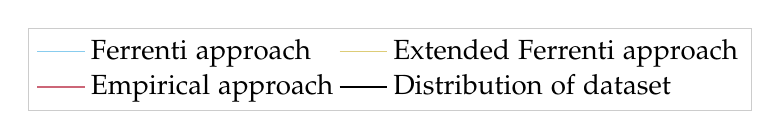
\begin{tikzpicture}

\definecolor{color0}{rgb}{0.866666666666667,0.8,0.466666666666667}
\definecolor{color1}{rgb}{0.533333333333333,0.8,0.933333333333333}
\definecolor{color3}{rgb}{0.8,0.4,0.466666666666667}
\begin{axis}[%
 hide axis,
 xmin=0,
 xmax=1,
 ymin=0,
 ymax=1,
 legend columns=2,
 legend cell align={left},
 legend style={
   fill opacity=1,
   draw opacity=1,
   text opacity=1,
   align=center,
   anchor=north,
   draw=white!80!black
 },
 ]
 \addlegendimage{semithick, color1}
 \addlegendentry{Ferrenti approach};
 \addlegendimage{semithick, color0}
 \addlegendentry{Extended Ferrenti approach};
 \addlegendimage{semithick, color3}
 \addlegendentry{Empirical approach};
 \addlegendimage{semithick, black}
 \addlegendentry{Distribution of dataset};
 \end{axis}

\end{tikzpicture}

\end{subfigure}
\begin{subfigure}[b]{0.45\textwidth}
    \scalebox{0.85}{% This file was created with tikzplotlib v0.9.16.
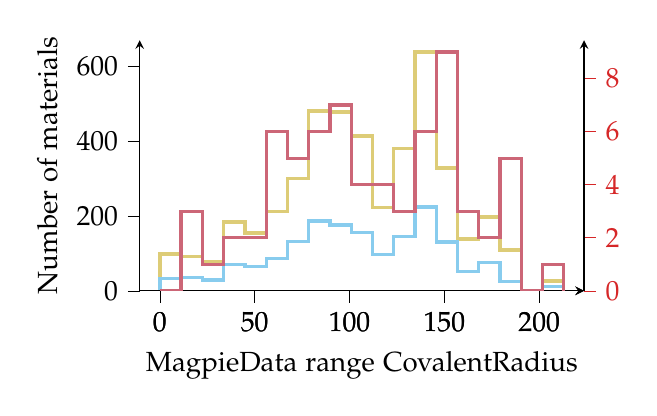
\begin{tikzpicture}

\definecolor{color0}{rgb}{0.866666666666667,0.8,0.466666666666667}
\definecolor{color1}{rgb}{0.533333333333333,0.8,0.933333333333333}
\definecolor{color2}{rgb}{0.83921568627451,0.152941176470588,0.156862745098039}
\definecolor{color3}{rgb}{0.8,0.4,0.466666666666667}

\begin{axis}[
height=1.875590092707901in,
legend cell align={left},
legend style={fill opacity=0.8, draw opacity=1, text opacity=1, draw=white!80!black},
tick align=outside,
tick pos=left,
width=2.8444876158848764in,
x grid style={white!69.0196078431373!black},
xlabel={MagpieData range CovalentRadius},
xmin=-10.65, xmax=223.65,
xtick style={color=black},
y grid style={white!69.0196078431373!black},
ylabel={Number of materials},
ymin=0, ymax=668.85,
ytick style={color=black}
]
\path [draw=color0, very thick]
(axis cs:0,0)
--(axis cs:0,98)
--(axis cs:11.2105263157895,98)
--(axis cs:11.2105263157895,92)
--(axis cs:22.4210526315789,92)
--(axis cs:22.4210526315789,79)
--(axis cs:33.6315789473684,79)
--(axis cs:33.6315789473684,184)
--(axis cs:44.8421052631579,184)
--(axis cs:44.8421052631579,154)
--(axis cs:56.0526315789474,154)
--(axis cs:56.0526315789474,211)
--(axis cs:67.2631578947368,211)
--(axis cs:67.2631578947368,300)
--(axis cs:78.4736842105263,300)
--(axis cs:78.4736842105263,480)
--(axis cs:89.6842105263158,480)
--(axis cs:89.6842105263158,477)
--(axis cs:100.894736842105,477)
--(axis cs:100.894736842105,413)
--(axis cs:112.105263157895,413)
--(axis cs:112.105263157895,223)
--(axis cs:123.315789473684,223)
--(axis cs:123.315789473684,379)
--(axis cs:134.526315789474,379)
--(axis cs:134.526315789474,637)
--(axis cs:145.736842105263,637)
--(axis cs:145.736842105263,328)
--(axis cs:156.947368421053,328)
--(axis cs:156.947368421053,138)
--(axis cs:168.157894736842,138)
--(axis cs:168.157894736842,197)
--(axis cs:179.368421052632,197)
--(axis cs:179.368421052632,109)
--(axis cs:190.578947368421,109)
--(axis cs:190.578947368421,0)
--(axis cs:201.789473684211,0)
--(axis cs:201.789473684211,26)
--(axis cs:213,26)
--(axis cs:213,0);

\path [draw=color1, very thick]
(axis cs:0,0)
--(axis cs:0,32)
--(axis cs:11.2105263157895,32)
--(axis cs:11.2105263157895,36)
--(axis cs:22.4210526315789,36)
--(axis cs:22.4210526315789,29)
--(axis cs:33.6315789473684,29)
--(axis cs:33.6315789473684,71)
--(axis cs:44.8421052631579,71)
--(axis cs:44.8421052631579,65)
--(axis cs:56.0526315789474,65)
--(axis cs:56.0526315789474,87)
--(axis cs:67.2631578947368,87)
--(axis cs:67.2631578947368,132)
--(axis cs:78.4736842105263,132)
--(axis cs:78.4736842105263,186)
--(axis cs:89.6842105263158,186)
--(axis cs:89.6842105263158,176)
--(axis cs:100.894736842105,176)
--(axis cs:100.894736842105,156)
--(axis cs:112.105263157895,156)
--(axis cs:112.105263157895,97)
--(axis cs:123.315789473684,97)
--(axis cs:123.315789473684,145)
--(axis cs:134.526315789474,145)
--(axis cs:134.526315789474,224)
--(axis cs:145.736842105263,224)
--(axis cs:145.736842105263,130)
--(axis cs:156.947368421053,130)
--(axis cs:156.947368421053,51)
--(axis cs:168.157894736842,51)
--(axis cs:168.157894736842,76)
--(axis cs:179.368421052632,76)
--(axis cs:179.368421052632,25)
--(axis cs:190.578947368421,25)
--(axis cs:190.578947368421,0)
--(axis cs:201.789473684211,0)
--(axis cs:201.789473684211,11)
--(axis cs:213,11)
--(axis cs:213,0);

\end{axis}

\begin{axis}[
axis y line=right,
height=1.875590092707901in,
tick align=outside,
width=2.8444876158848764in,
x grid style={white!69.0196078431373!black},
xmin=-10.65, xmax=223.65,
xtick pos=left,
xtick style={color=black},
y grid style={white!69.0196078431373!black},
ymin=0, ymax=9.45,
ytick pos=right,
ytick style={color=color2},
yticklabel style={anchor=west, color2}
]
\path [draw=color3, very thick]
(axis cs:0,0)
--(axis cs:0,0)
--(axis cs:11.2105263157895,0)
--(axis cs:11.2105263157895,3)
--(axis cs:22.4210526315789,3)
--(axis cs:22.4210526315789,1)
--(axis cs:33.6315789473684,1)
--(axis cs:33.6315789473684,2)
--(axis cs:44.8421052631579,2)
--(axis cs:44.8421052631579,2)
--(axis cs:56.0526315789474,2)
--(axis cs:56.0526315789474,6)
--(axis cs:67.2631578947368,6)
--(axis cs:67.2631578947368,5)
--(axis cs:78.4736842105263,5)
--(axis cs:78.4736842105263,6)
--(axis cs:89.6842105263158,6)
--(axis cs:89.6842105263158,7)
--(axis cs:100.894736842105,7)
--(axis cs:100.894736842105,4)
--(axis cs:112.105263157895,4)
--(axis cs:112.105263157895,4)
--(axis cs:123.315789473684,4)
--(axis cs:123.315789473684,3)
--(axis cs:134.526315789474,3)
--(axis cs:134.526315789474,6)
--(axis cs:145.736842105263,6)
--(axis cs:145.736842105263,9)
--(axis cs:156.947368421053,9)
--(axis cs:156.947368421053,3)
--(axis cs:168.157894736842,3)
--(axis cs:168.157894736842,2)
--(axis cs:179.368421052632,2)
--(axis cs:179.368421052632,5)
--(axis cs:190.578947368421,5)
--(axis cs:190.578947368421,0)
--(axis cs:201.789473684211,0)
--(axis cs:201.789473684211,1)
--(axis cs:213,1)
--(axis cs:213,0);
\end{axis}

\end{tikzpicture}
}
    \subcaption{}
\end{subfigure}
\begin{subfigure}[b]{0.45\textwidth}
    \scalebox{0.85}{% This file was created with tikzplotlib v0.9.16.
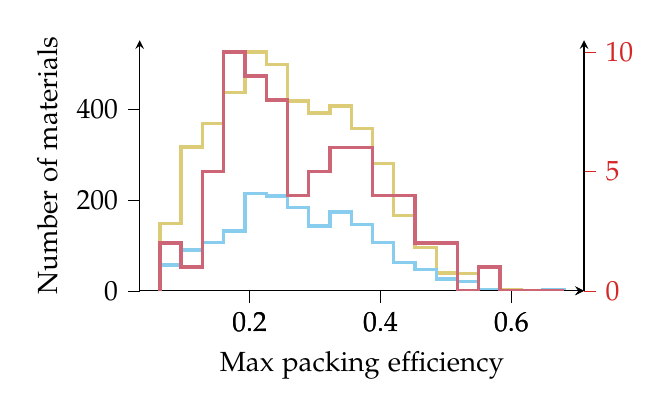
\begin{tikzpicture}

\definecolor{color0}{rgb}{0.866666666666667,0.8,0.466666666666667}
\definecolor{color1}{rgb}{0.533333333333333,0.8,0.933333333333333}
\definecolor{color2}{rgb}{0.83921568627451,0.152941176470588,0.156862745098039}
\definecolor{color3}{rgb}{0.8,0.4,0.466666666666667}

\begin{axis}[
height=1.875590092707901in,
legend cell align={left},
legend style={fill opacity=0.8, draw opacity=1, text opacity=1, draw=white!80!black},
tick align=outside,
tick pos=left,
width=2.8444876158848764in,
x grid style={white!69.0196078431373!black},
xlabel={Max packing efficiency},
xmin=0.0318178138255053, xmax=0.711048901957466,
xtick style={color=black},
y grid style={white!69.0196078431373!black},
ylabel={Number of materials},
ymin=0, ymax=552.3,
ytick style={color=black}
]
\path [draw=color0, very thick]
(axis cs:0.0626919541951399,0)
--(axis cs:0.0626919541951399,148)
--(axis cs:0.0951910493210711,148)
--(axis cs:0.0951910493210711,317)
--(axis cs:0.127690144447002,317)
--(axis cs:0.127690144447002,369)
--(axis cs:0.160189239572933,369)
--(axis cs:0.160189239572933,437)
--(axis cs:0.192688334698864,437)
--(axis cs:0.192688334698864,526)
--(axis cs:0.225187429824796,526)
--(axis cs:0.225187429824796,498)
--(axis cs:0.257686524950727,498)
--(axis cs:0.257686524950727,418)
--(axis cs:0.290185620076658,418)
--(axis cs:0.290185620076658,392)
--(axis cs:0.322684715202589,392)
--(axis cs:0.322684715202589,407)
--(axis cs:0.35518381032852,407)
--(axis cs:0.35518381032852,358)
--(axis cs:0.387682905454451,358)
--(axis cs:0.387682905454451,281)
--(axis cs:0.420182000580382,281)
--(axis cs:0.420182000580382,166)
--(axis cs:0.452681095706314,166)
--(axis cs:0.452681095706314,95)
--(axis cs:0.485180190832245,95)
--(axis cs:0.485180190832245,39)
--(axis cs:0.517679285958176,39)
--(axis cs:0.517679285958176,38)
--(axis cs:0.550178381084107,38)
--(axis cs:0.550178381084107,3)
--(axis cs:0.582677476210038,3)
--(axis cs:0.582677476210038,2)
--(axis cs:0.615176571335969,2)
--(axis cs:0.615176571335969,1)
--(axis cs:0.6476756664619,1)
--(axis cs:0.6476756664619,3)
--(axis cs:0.680174761587832,3)
--(axis cs:0.680174761587832,0);

\path [draw=color1, very thick]
(axis cs:0.0626919541951399,0)
--(axis cs:0.0626919541951399,57)
--(axis cs:0.0951910493210711,57)
--(axis cs:0.0951910493210711,90)
--(axis cs:0.127690144447002,90)
--(axis cs:0.127690144447002,107)
--(axis cs:0.160189239572933,107)
--(axis cs:0.160189239572933,132)
--(axis cs:0.192688334698864,132)
--(axis cs:0.192688334698864,215)
--(axis cs:0.225187429824796,215)
--(axis cs:0.225187429824796,209)
--(axis cs:0.257686524950727,209)
--(axis cs:0.257686524950727,183)
--(axis cs:0.290185620076658,183)
--(axis cs:0.290185620076658,143)
--(axis cs:0.322684715202589,143)
--(axis cs:0.322684715202589,174)
--(axis cs:0.35518381032852,174)
--(axis cs:0.35518381032852,146)
--(axis cs:0.387682905454451,146)
--(axis cs:0.387682905454451,106)
--(axis cs:0.420182000580382,106)
--(axis cs:0.420182000580382,63)
--(axis cs:0.452681095706314,63)
--(axis cs:0.452681095706314,47)
--(axis cs:0.485180190832245,47)
--(axis cs:0.485180190832245,26)
--(axis cs:0.517679285958176,26)
--(axis cs:0.517679285958176,21)
--(axis cs:0.550178381084107,21)
--(axis cs:0.550178381084107,3)
--(axis cs:0.582677476210038,3)
--(axis cs:0.582677476210038,0)
--(axis cs:0.615176571335969,0)
--(axis cs:0.615176571335969,0)
--(axis cs:0.6476756664619,0)
--(axis cs:0.6476756664619,3)
--(axis cs:0.680174761587832,3)
--(axis cs:0.680174761587832,0);

\end{axis}

\begin{axis}[
axis y line=right,
height=1.875590092707901in,
tick align=outside,
width=2.8444876158848764in,
x grid style={white!69.0196078431373!black},
xmin=0.0318178138255053, xmax=0.711048901957466,
xtick pos=left,
xtick style={color=black},
y grid style={white!69.0196078431373!black},
ymin=0, ymax=10.5,
ytick pos=right,
ytick style={color=color2},
yticklabel style={anchor=west, color=color2}
]
\path [draw=color3, very thick]
(axis cs:0.0626919541951399,0)
--(axis cs:0.0626919541951399,2)
--(axis cs:0.0951910493210711,2)
--(axis cs:0.0951910493210711,1)
--(axis cs:0.127690144447002,1)
--(axis cs:0.127690144447002,5)
--(axis cs:0.160189239572933,5)
--(axis cs:0.160189239572933,10)
--(axis cs:0.192688334698864,10)
--(axis cs:0.192688334698864,9)
--(axis cs:0.225187429824796,9)
--(axis cs:0.225187429824796,8)
--(axis cs:0.257686524950727,8)
--(axis cs:0.257686524950727,4)
--(axis cs:0.290185620076658,4)
--(axis cs:0.290185620076658,5)
--(axis cs:0.322684715202589,5)
--(axis cs:0.322684715202589,6)
--(axis cs:0.35518381032852,6)
--(axis cs:0.35518381032852,6)
--(axis cs:0.387682905454451,6)
--(axis cs:0.387682905454451,4)
--(axis cs:0.420182000580382,4)
--(axis cs:0.420182000580382,4)
--(axis cs:0.452681095706314,4)
--(axis cs:0.452681095706314,2)
--(axis cs:0.485180190832245,2)
--(axis cs:0.485180190832245,2)
--(axis cs:0.517679285958176,2)
--(axis cs:0.517679285958176,0)
--(axis cs:0.550178381084107,0)
--(axis cs:0.550178381084107,1)
--(axis cs:0.582677476210038,1)
--(axis cs:0.582677476210038,0)
--(axis cs:0.615176571335969,0)
--(axis cs:0.615176571335969,0)
--(axis cs:0.6476756664619,0)
--(axis cs:0.6476756664619,0)
--(axis cs:0.680174761587832,0)
--(axis cs:0.680174761587832,0);
\end{axis}

\end{tikzpicture}
}
    \subcaption{}
\end{subfigure}%

\begin{subfigure}[b]{0.45\textwidth}
    \scalebox{0.85}{% This file was created with tikzplotlib v0.9.16.
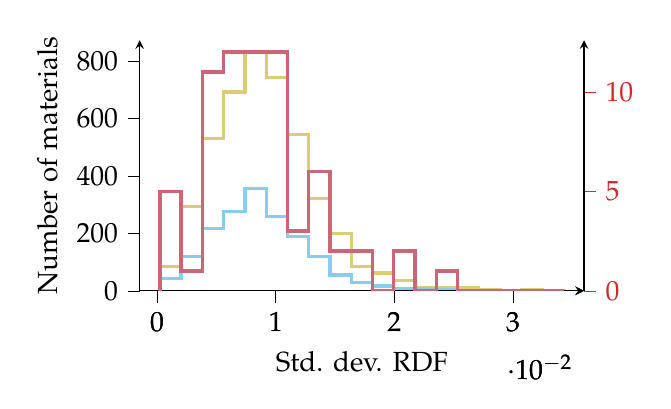
\begin{tikzpicture}

\definecolor{color0}{rgb}{0.866666666666667,0.8,0.466666666666667}
\definecolor{color1}{rgb}{0.533333333333333,0.8,0.933333333333333}
\definecolor{color2}{rgb}{0.83921568627451,0.152941176470588,0.156862745098039}
\definecolor{color3}{rgb}{0.8,0.4,0.466666666666667}

\begin{axis}[
height=1.875590092707901in,
legend cell align={left},
legend style={fill opacity=0.8, draw opacity=1, text opacity=1, draw=white!80!black},
tick align=outside,
tick pos=left,
width=2.8444876158848764in,
x grid style={white!69.0196078431373!black},
xlabel={Std. dev. RDF},
xmin=-0.00146657305751061, xmax=0.0359919745342756,
xtick style={color=black},
y grid style={white!69.0196078431373!black},
ylabel={Number of materials},
ymin=0, ymax=873.6,
ytick style={color=black}
]
\path [draw=color0, very thick]
(axis cs:0.000236088196661485,0)
--(axis cs:0.000236088196661485,84)
--(axis cs:0.00202836320105317,84)
--(axis cs:0.00202836320105317,293)
--(axis cs:0.00382063820544485,293)
--(axis cs:0.00382063820544485,530)
--(axis cs:0.00561291320983653,530)
--(axis cs:0.00561291320983653,693)
--(axis cs:0.00740518821422822,693)
--(axis cs:0.00740518821422822,832)
--(axis cs:0.0091974632186199,832)
--(axis cs:0.0091974632186199,743)
--(axis cs:0.0109897382230116,743)
--(axis cs:0.0109897382230116,544)
--(axis cs:0.0127820132274033,544)
--(axis cs:0.0127820132274033,322)
--(axis cs:0.0145742882317949,322)
--(axis cs:0.0145742882317949,200)
--(axis cs:0.0163665632361866,200)
--(axis cs:0.0163665632361866,85)
--(axis cs:0.0181588382405783,85)
--(axis cs:0.0181588382405783,62)
--(axis cs:0.01995111324497,62)
--(axis cs:0.01995111324497,37)
--(axis cs:0.0217433882493617,37)
--(axis cs:0.0217433882493617,11)
--(axis cs:0.0235356632537534,11)
--(axis cs:0.0235356632537534,12)
--(axis cs:0.025327938258145,12)
--(axis cs:0.025327938258145,10)
--(axis cs:0.0271202132625367,10)
--(axis cs:0.0271202132625367,5)
--(axis cs:0.0289124882669284,5)
--(axis cs:0.0289124882669284,0)
--(axis cs:0.0307047632713201,0)
--(axis cs:0.0307047632713201,3)
--(axis cs:0.0324970382757118,3)
--(axis cs:0.0324970382757118,1)
--(axis cs:0.0342893132801035,1)
--(axis cs:0.0342893132801035,0);

\path [draw=color1, very thick]
(axis cs:0.000236088196661485,0)
--(axis cs:0.000236088196661485,42)
--(axis cs:0.00202836320105317,42)
--(axis cs:0.00202836320105317,119)
--(axis cs:0.00382063820544485,119)
--(axis cs:0.00382063820544485,217)
--(axis cs:0.00561291320983653,217)
--(axis cs:0.00561291320983653,276)
--(axis cs:0.00740518821422822,276)
--(axis cs:0.00740518821422822,356)
--(axis cs:0.0091974632186199,356)
--(axis cs:0.0091974632186199,260)
--(axis cs:0.0109897382230116,260)
--(axis cs:0.0109897382230116,190)
--(axis cs:0.0127820132274033,190)
--(axis cs:0.0127820132274033,119)
--(axis cs:0.0145742882317949,119)
--(axis cs:0.0145742882317949,55)
--(axis cs:0.0163665632361866,55)
--(axis cs:0.0163665632361866,28)
--(axis cs:0.0181588382405783,28)
--(axis cs:0.0181588382405783,17)
--(axis cs:0.01995111324497,17)
--(axis cs:0.01995111324497,7)
--(axis cs:0.0217433882493617,7)
--(axis cs:0.0217433882493617,8)
--(axis cs:0.0235356632537534,8)
--(axis cs:0.0235356632537534,4)
--(axis cs:0.025327938258145,4)
--(axis cs:0.025327938258145,0)
--(axis cs:0.0271202132625367,0)
--(axis cs:0.0271202132625367,2)
--(axis cs:0.0289124882669284,2)
--(axis cs:0.0289124882669284,1)
--(axis cs:0.0307047632713201,1)
--(axis cs:0.0307047632713201,1)
--(axis cs:0.0324970382757118,1)
--(axis cs:0.0324970382757118,0)
--(axis cs:0.0342893132801035,0)
--(axis cs:0.0342893132801035,0);

\end{axis}

\begin{axis}[
axis y line=right,
height=1.875590092707901in,
tick align=outside,
width=2.8444876158848764in,
x grid style={white!69.0196078431373!black},
xmin=-0.00146657305751061, xmax=0.0359919745342756,
xtick pos=left,
xtick style={color=black},
y grid style={white!69.0196078431373!black},
ymin=0, ymax=12.6,
ytick pos=right,
ytick style={color=color2},
yticklabel style={anchor=west, color=color2}
]
\path [draw=color3, very thick]
(axis cs:0.000236088196661485,0)
--(axis cs:0.000236088196661485,5)
--(axis cs:0.00202836320105317,5)
--(axis cs:0.00202836320105317,1)
--(axis cs:0.00382063820544485,1)
--(axis cs:0.00382063820544485,11)
--(axis cs:0.00561291320983653,11)
--(axis cs:0.00561291320983653,12)
--(axis cs:0.00740518821422822,12)
--(axis cs:0.00740518821422822,12)
--(axis cs:0.0091974632186199,12)
--(axis cs:0.0091974632186199,12)
--(axis cs:0.0109897382230116,12)
--(axis cs:0.0109897382230116,3)
--(axis cs:0.0127820132274033,3)
--(axis cs:0.0127820132274033,6)
--(axis cs:0.0145742882317949,6)
--(axis cs:0.0145742882317949,2)
--(axis cs:0.0163665632361866,2)
--(axis cs:0.0163665632361866,2)
--(axis cs:0.0181588382405783,2)
--(axis cs:0.0181588382405783,0)
--(axis cs:0.01995111324497,0)
--(axis cs:0.01995111324497,2)
--(axis cs:0.0217433882493617,2)
--(axis cs:0.0217433882493617,0)
--(axis cs:0.0235356632537534,0)
--(axis cs:0.0235356632537534,1)
--(axis cs:0.025327938258145,1)
--(axis cs:0.025327938258145,0)
--(axis cs:0.0271202132625367,0)
--(axis cs:0.0271202132625367,0)
--(axis cs:0.0289124882669284,0)
--(axis cs:0.0289124882669284,0)
--(axis cs:0.0307047632713201,0)
--(axis cs:0.0307047632713201,0)
--(axis cs:0.0324970382757118,0)
--(axis cs:0.0324970382757118,0)
--(axis cs:0.0342893132801035,0)
--(axis cs:0.0342893132801035,0);
\end{axis}

\end{tikzpicture}
}
    \subcaption{}
\end{subfigure}
\begin{subfigure}[b]{0.45\textwidth}
    \scalebox{0.85}{% This file was created with tikzplotlib v0.9.16.
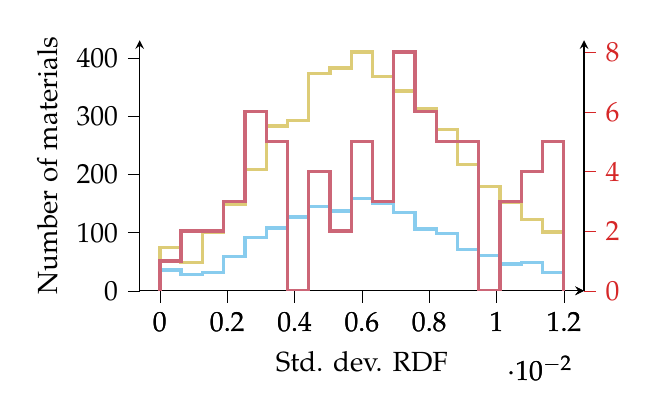
\begin{tikzpicture}

\definecolor{color0}{rgb}{0.866666666666667,0.8,0.466666666666667}
\definecolor{color1}{rgb}{0.533333333333333,0.8,0.933333333333333}
\definecolor{color2}{rgb}{0.83921568627451,0.152941176470588,0.156862745098039}
\definecolor{color3}{rgb}{0.8,0.4,0.466666666666667}

\begin{axis}[
height=1.875590092707901in,
legend cell align={left},
legend style={fill opacity=0.8, draw opacity=1, text opacity=1, draw=white!80!black},
tick align=outside,
tick pos=left,
width=2.8444876158848764in,
x grid style={white!69.0196078431373!black},
xlabel={Std. dev. RDF},
xmin=-0.000599766697946528, xmax=0.0125951006568771,
xtick style={color=black},
y grid style={white!69.0196078431373!black},
ylabel={Number of materials},
ymin=0, ymax=430.5,
ytick style={color=black}
]
\path [draw=color0, very thick]
(axis cs:0,0)
--(axis cs:0,74)
--(axis cs:0.000631333366259504,74)
--(axis cs:0.000631333366259504,49)
--(axis cs:0.00126266673251901,49)
--(axis cs:0.00126266673251901,100)
--(axis cs:0.00189400009877851,100)
--(axis cs:0.00189400009877851,148)
--(axis cs:0.00252533346503801,148)
--(axis cs:0.00252533346503801,208)
--(axis cs:0.00315666683129752,208)
--(axis cs:0.00315666683129752,283)
--(axis cs:0.00378800019755702,283)
--(axis cs:0.00378800019755702,292)
--(axis cs:0.00441933356381652,292)
--(axis cs:0.00441933356381652,373)
--(axis cs:0.00505066693007603,373)
--(axis cs:0.00505066693007603,383)
--(axis cs:0.00568200029633553,383)
--(axis cs:0.00568200029633553,410)
--(axis cs:0.00631333366259504,410)
--(axis cs:0.00631333366259504,368)
--(axis cs:0.00694466702885454,368)
--(axis cs:0.00694466702885454,343)
--(axis cs:0.00757600039511404,343)
--(axis cs:0.00757600039511404,313)
--(axis cs:0.00820733376137354,313)
--(axis cs:0.00820733376137354,277)
--(axis cs:0.00883866712763305,277)
--(axis cs:0.00883866712763305,217)
--(axis cs:0.00947000049389255,217)
--(axis cs:0.00947000049389255,179)
--(axis cs:0.0101013338601521,179)
--(axis cs:0.0101013338601521,152)
--(axis cs:0.0107326672264116,152)
--(axis cs:0.0107326672264116,122)
--(axis cs:0.0113640005926711,122)
--(axis cs:0.0113640005926711,101)
--(axis cs:0.0119953339589306,101)
--(axis cs:0.0119953339589306,0);

\path [draw=color1, very thick]
(axis cs:0,0)
--(axis cs:0,36)
--(axis cs:0.000631333366259504,36)
--(axis cs:0.000631333366259504,28)
--(axis cs:0.00126266673251901,28)
--(axis cs:0.00126266673251901,31)
--(axis cs:0.00189400009877851,31)
--(axis cs:0.00189400009877851,59)
--(axis cs:0.00252533346503801,59)
--(axis cs:0.00252533346503801,92)
--(axis cs:0.00315666683129752,92)
--(axis cs:0.00315666683129752,108)
--(axis cs:0.00378800019755702,108)
--(axis cs:0.00378800019755702,127)
--(axis cs:0.00441933356381652,127)
--(axis cs:0.00441933356381652,145)
--(axis cs:0.00505066693007603,145)
--(axis cs:0.00505066693007603,137)
--(axis cs:0.00568200029633553,137)
--(axis cs:0.00568200029633553,158)
--(axis cs:0.00631333366259504,158)
--(axis cs:0.00631333366259504,151)
--(axis cs:0.00694466702885454,151)
--(axis cs:0.00694466702885454,135)
--(axis cs:0.00757600039511404,135)
--(axis cs:0.00757600039511404,106)
--(axis cs:0.00820733376137354,106)
--(axis cs:0.00820733376137354,98)
--(axis cs:0.00883866712763305,98)
--(axis cs:0.00883866712763305,71)
--(axis cs:0.00947000049389255,71)
--(axis cs:0.00947000049389255,61)
--(axis cs:0.0101013338601521,61)
--(axis cs:0.0101013338601521,46)
--(axis cs:0.0107326672264116,46)
--(axis cs:0.0107326672264116,49)
--(axis cs:0.0113640005926711,49)
--(axis cs:0.0113640005926711,31)
--(axis cs:0.0119953339589306,31)
--(axis cs:0.0119953339589306,0);

\end{axis}

\begin{axis}[
axis y line=right,
height=1.875590092707901in,
tick align=outside,
width=2.8444876158848764in,
x grid style={white!69.0196078431373!black},
xmin=-0.000599766697946528, xmax=0.0125951006568771,
xtick pos=left,
xtick style={color=black},
y grid style={white!69.0196078431373!black},
ymin=0, ymax=8.4,
ytick pos=right,
ytick style={color=color2},
yticklabel style={anchor=west, color=color2}
]
\path [draw=color3, very thick]
(axis cs:0,0)
--(axis cs:0,1)
--(axis cs:0.000631333366259504,1)
--(axis cs:0.000631333366259504,2)
--(axis cs:0.00126266673251901,2)
--(axis cs:0.00126266673251901,2)
--(axis cs:0.00189400009877851,2)
--(axis cs:0.00189400009877851,3)
--(axis cs:0.00252533346503801,3)
--(axis cs:0.00252533346503801,6)
--(axis cs:0.00315666683129752,6)
--(axis cs:0.00315666683129752,5)
--(axis cs:0.00378800019755702,5)
--(axis cs:0.00378800019755702,0)
--(axis cs:0.00441933356381652,0)
--(axis cs:0.00441933356381652,4)
--(axis cs:0.00505066693007603,4)
--(axis cs:0.00505066693007603,2)
--(axis cs:0.00568200029633553,2)
--(axis cs:0.00568200029633553,5)
--(axis cs:0.00631333366259504,5)
--(axis cs:0.00631333366259504,3)
--(axis cs:0.00694466702885454,3)
--(axis cs:0.00694466702885454,8)
--(axis cs:0.00757600039511404,8)
--(axis cs:0.00757600039511404,6)
--(axis cs:0.00820733376137354,6)
--(axis cs:0.00820733376137354,5)
--(axis cs:0.00883866712763305,5)
--(axis cs:0.00883866712763305,5)
--(axis cs:0.00947000049389255,5)
--(axis cs:0.00947000049389255,0)
--(axis cs:0.0101013338601521,0)
--(axis cs:0.0101013338601521,3)
--(axis cs:0.0107326672264116,3)
--(axis cs:0.0107326672264116,4)
--(axis cs:0.0113640005926711,4)
--(axis cs:0.0113640005926711,5)
--(axis cs:0.0119953339589306,5)
--(axis cs:0.0119953339589306,0);
\end{axis}

\end{tikzpicture}
}
    \subcaption{}
\end{subfigure}%
\end{figure}

Figure~\ref{fig:histograms_supp} displays the number of predicted suitable materials for all approaches (all ML methods in an approach agree to a $0.75$ confidence level) as a function of the (a) covalent radius of the elements in the composition, (b) maximum packing efficiency, and standard deviation of the radial distribution function (RDF) with center at (c) $2.0$ and (d) $3.0$. The corresponding figure in the main text shows the standard deviation of the RDF with Gaussian center at $1.0$. 
%Several observations can be made based on the histograms. 
Panels (e) chemical environment site fingerprint, (f) crystal fingerprint and (g) OP site fingerprint are related to bond orientational parameters, while (h) shows the material band gaps referenced to the normalized mean of the entire data set.  

\begin{figure}[ht!]\ContinuedFloat
\begin{subfigure}[b]{0.45\textwidth}
    \scalebox{0.85}{% This file was created with tikzplotlib v0.9.16.
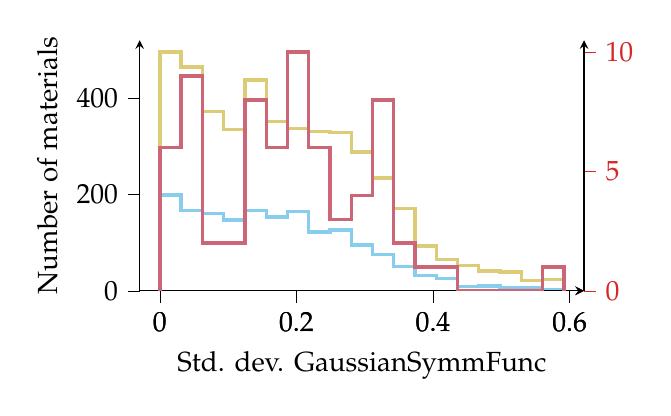
\begin{tikzpicture}

\definecolor{color0}{rgb}{0.866666666666667,0.8,0.466666666666667}
\definecolor{color1}{rgb}{0.533333333333333,0.8,0.933333333333333}
\definecolor{color2}{rgb}{0.83921568627451,0.152941176470588,0.156862745098039}
\definecolor{color3}{rgb}{0.8,0.4,0.466666666666667}

\begin{axis}[
height=1.875590092707901in,
legend cell align={left},
legend style={fill opacity=0.8, draw opacity=1, text opacity=1, draw=white!80!black},
tick align=outside,
tick pos=left,
width=2.8444876158848764in,
x grid style={white!69.0196078431373!black},
xlabel={Std. dev. GaussianSymmFunc},
xmin=-0.0295818294063694, xmax=0.621218417533758,
xtick style={color=black},
y grid style={white!69.0196078431373!black},
ylabel={Number of materials},
ymin=0, ymax=519.75,
ytick style={color=black}
]
\path [draw=color0, very thick]
(axis cs:0,0)
--(axis cs:0,495)
--(axis cs:0.0311387677961784,495)
--(axis cs:0.0311387677961784,464)
--(axis cs:0.0622775355923567,464)
--(axis cs:0.0622775355923567,372)
--(axis cs:0.0934163033885351,372)
--(axis cs:0.0934163033885351,334)
--(axis cs:0.124555071184713,334)
--(axis cs:0.124555071184713,437)
--(axis cs:0.155693838980892,437)
--(axis cs:0.155693838980892,351)
--(axis cs:0.18683260677707,351)
--(axis cs:0.18683260677707,337)
--(axis cs:0.217971374573249,337)
--(axis cs:0.217971374573249,331)
--(axis cs:0.249110142369427,331)
--(axis cs:0.249110142369427,329)
--(axis cs:0.280248910165605,329)
--(axis cs:0.280248910165605,288)
--(axis cs:0.311387677961784,288)
--(axis cs:0.311387677961784,234)
--(axis cs:0.342526445757962,234)
--(axis cs:0.342526445757962,170)
--(axis cs:0.37366521355414,170)
--(axis cs:0.37366521355414,93)
--(axis cs:0.404803981350319,93)
--(axis cs:0.404803981350319,65)
--(axis cs:0.435942749146497,65)
--(axis cs:0.435942749146497,52)
--(axis cs:0.467081516942676,52)
--(axis cs:0.467081516942676,41)
--(axis cs:0.498220284738854,41)
--(axis cs:0.498220284738854,39)
--(axis cs:0.529359052535032,39)
--(axis cs:0.529359052535032,22)
--(axis cs:0.560497820331211,22)
--(axis cs:0.560497820331211,23)
--(axis cs:0.591636588127389,23)
--(axis cs:0.591636588127389,0);

\path [draw=color1, very thick]
(axis cs:0,0)
--(axis cs:0,199)
--(axis cs:0.0311387677961784,199)
--(axis cs:0.0311387677961784,167)
--(axis cs:0.0622775355923567,167)
--(axis cs:0.0622775355923567,160)
--(axis cs:0.0934163033885351,160)
--(axis cs:0.0934163033885351,147)
--(axis cs:0.124555071184713,147)
--(axis cs:0.124555071184713,166)
--(axis cs:0.155693838980892,166)
--(axis cs:0.155693838980892,153)
--(axis cs:0.18683260677707,153)
--(axis cs:0.18683260677707,164)
--(axis cs:0.217971374573249,164)
--(axis cs:0.217971374573249,122)
--(axis cs:0.249110142369427,122)
--(axis cs:0.249110142369427,126)
--(axis cs:0.280248910165605,126)
--(axis cs:0.280248910165605,95)
--(axis cs:0.311387677961784,95)
--(axis cs:0.311387677961784,75)
--(axis cs:0.342526445757962,75)
--(axis cs:0.342526445757962,50)
--(axis cs:0.37366521355414,50)
--(axis cs:0.37366521355414,32)
--(axis cs:0.404803981350319,32)
--(axis cs:0.404803981350319,26)
--(axis cs:0.435942749146497,26)
--(axis cs:0.435942749146497,9)
--(axis cs:0.467081516942676,9)
--(axis cs:0.467081516942676,10)
--(axis cs:0.498220284738854,10)
--(axis cs:0.498220284738854,7)
--(axis cs:0.529359052535032,7)
--(axis cs:0.529359052535032,7)
--(axis cs:0.560497820331211,7)
--(axis cs:0.560497820331211,3)
--(axis cs:0.591636588127389,3)
--(axis cs:0.591636588127389,0);

\end{axis}

\begin{axis}[
axis y line=right,
height=1.875590092707901in,
tick align=outside,
width=2.8444876158848764in,
x grid style={white!69.0196078431373!black},
xmin=-0.0295818294063694, xmax=0.621218417533758,
xtick pos=left,
xtick style={color=black},
y grid style={white!69.0196078431373!black},
ymin=0, ymax=10.5,
ytick pos=right,
ytick style={color=color2},
yticklabel style={anchor=west, color=color2}
]
\path [draw=color3, very thick]
(axis cs:0,0)
--(axis cs:0,6)
--(axis cs:0.0311387677961784,6)
--(axis cs:0.0311387677961784,9)
--(axis cs:0.0622775355923567,9)
--(axis cs:0.0622775355923567,2)
--(axis cs:0.0934163033885351,2)
--(axis cs:0.0934163033885351,2)
--(axis cs:0.124555071184713,2)
--(axis cs:0.124555071184713,8)
--(axis cs:0.155693838980892,8)
--(axis cs:0.155693838980892,6)
--(axis cs:0.18683260677707,6)
--(axis cs:0.18683260677707,10)
--(axis cs:0.217971374573249,10)
--(axis cs:0.217971374573249,6)
--(axis cs:0.249110142369427,6)
--(axis cs:0.249110142369427,3)
--(axis cs:0.280248910165605,3)
--(axis cs:0.280248910165605,4)
--(axis cs:0.311387677961784,4)
--(axis cs:0.311387677961784,8)
--(axis cs:0.342526445757962,8)
--(axis cs:0.342526445757962,2)
--(axis cs:0.37366521355414,2)
--(axis cs:0.37366521355414,1)
--(axis cs:0.404803981350319,1)
--(axis cs:0.404803981350319,1)
--(axis cs:0.435942749146497,1)
--(axis cs:0.435942749146497,0)
--(axis cs:0.467081516942676,0)
--(axis cs:0.467081516942676,0)
--(axis cs:0.498220284738854,0)
--(axis cs:0.498220284738854,0)
--(axis cs:0.529359052535032,0)
--(axis cs:0.529359052535032,0)
--(axis cs:0.560497820331211,0)
--(axis cs:0.560497820331211,1)
--(axis cs:0.591636588127389,1)
--(axis cs:0.591636588127389,0);
\end{axis}

\end{tikzpicture}
}
    \subcaption{}
\end{subfigure}
\begin{subfigure}[b]{0.45\textwidth}
    \scalebox{0.85}{% This file was created with tikzplotlib v0.9.16.
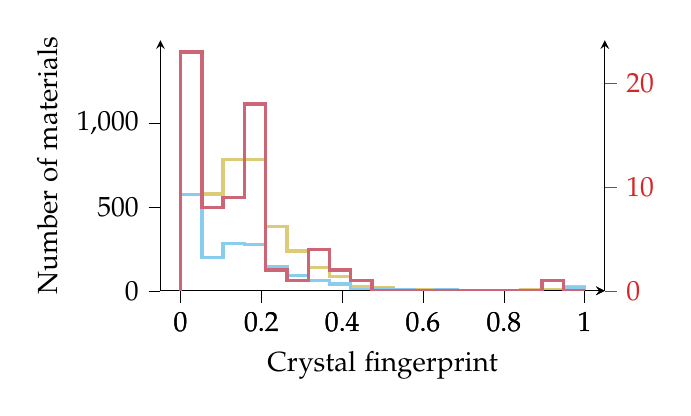
\begin{tikzpicture}

\definecolor{color0}{rgb}{0.866666666666667,0.8,0.466666666666667}
\definecolor{color1}{rgb}{0.533333333333333,0.8,0.933333333333333}
\definecolor{color2}{rgb}{0.83921568627451,0.152941176470588,0.156862745098039}
\definecolor{color3}{rgb}{0.8,0.4,0.466666666666667}

\begin{axis}[
height=1.875590092707901in,
legend cell align={left},
legend style={fill opacity=0.8, draw opacity=1, text opacity=1, draw=white!80!black},
tick align=outside,
tick pos=left,
width=2.8444876158848764in,
x grid style={white!69.0196078431373!black},
xlabel={Crystal fingerprint},
xmin=-0.05, xmax=1.05,
xtick style={color=black},
y grid style={white!69.0196078431373!black},
ylabel={Number of materials},
ymin=0, ymax=1492.05,
ytick style={color=black}
]
\path [draw=color0, very thick]
(axis cs:0,0)
--(axis cs:0,1421)
--(axis cs:0.0526315789473684,1421)
--(axis cs:0.0526315789473684,577)
--(axis cs:0.105263157894737,577)
--(axis cs:0.105263157894737,780)
--(axis cs:0.157894736842105,780)
--(axis cs:0.157894736842105,781)
--(axis cs:0.210526315789474,781)
--(axis cs:0.210526315789474,382)
--(axis cs:0.263157894736842,382)
--(axis cs:0.263157894736842,237)
--(axis cs:0.315789473684211,237)
--(axis cs:0.315789473684211,138)
--(axis cs:0.368421052631579,138)
--(axis cs:0.368421052631579,86)
--(axis cs:0.421052631578947,86)
--(axis cs:0.421052631578947,22)
--(axis cs:0.473684210526316,22)
--(axis cs:0.473684210526316,18)
--(axis cs:0.526315789473684,18)
--(axis cs:0.526315789473684,5)
--(axis cs:0.578947368421053,5)
--(axis cs:0.578947368421053,5)
--(axis cs:0.631578947368421,5)
--(axis cs:0.631578947368421,7)
--(axis cs:0.684210526315789,7)
--(axis cs:0.684210526315789,1)
--(axis cs:0.736842105263158,1)
--(axis cs:0.736842105263158,0)
--(axis cs:0.789473684210526,0)
--(axis cs:0.789473684210526,3)
--(axis cs:0.842105263157895,3)
--(axis cs:0.842105263157895,7)
--(axis cs:0.894736842105263,7)
--(axis cs:0.894736842105263,5)
--(axis cs:0.947368421052632,5)
--(axis cs:0.947368421052632,26)
--(axis cs:1,26)
--(axis cs:1,0);

\path [draw=color1, very thick]
(axis cs:0,0)
--(axis cs:0,574)
--(axis cs:0.0526315789473684,574)
--(axis cs:0.0526315789473684,197)
--(axis cs:0.105263157894737,197)
--(axis cs:0.105263157894737,283)
--(axis cs:0.157894736842105,283)
--(axis cs:0.157894736842105,274)
--(axis cs:0.210526315789474,274)
--(axis cs:0.210526315789474,146)
--(axis cs:0.263157894736842,146)
--(axis cs:0.263157894736842,91)
--(axis cs:0.315789473684211,91)
--(axis cs:0.315789473684211,63)
--(axis cs:0.368421052631579,63)
--(axis cs:0.368421052631579,40)
--(axis cs:0.421052631578947,40)
--(axis cs:0.421052631578947,7)
--(axis cs:0.473684210526316,7)
--(axis cs:0.473684210526316,11)
--(axis cs:0.526315789473684,11)
--(axis cs:0.526315789473684,5)
--(axis cs:0.578947368421053,5)
--(axis cs:0.578947368421053,2)
--(axis cs:0.631578947368421,2)
--(axis cs:0.631578947368421,4)
--(axis cs:0.684210526315789,4)
--(axis cs:0.684210526315789,0)
--(axis cs:0.736842105263158,0)
--(axis cs:0.736842105263158,2)
--(axis cs:0.789473684210526,2)
--(axis cs:0.789473684210526,2)
--(axis cs:0.842105263157895,2)
--(axis cs:0.842105263157895,1)
--(axis cs:0.894736842105263,1)
--(axis cs:0.894736842105263,3)
--(axis cs:0.947368421052632,3)
--(axis cs:0.947368421052632,19)
--(axis cs:1,19)
--(axis cs:1,0);

\end{axis}

\begin{axis}[
axis y line=right,
height=1.875590092707901in,
tick align=outside,
width=2.8444876158848764in,
x grid style={white!69.0196078431373!black},
xmin=-0.05, xmax=1.05,
xtick pos=left,
xtick style={color=black},
y grid style={white!69.0196078431373!black},
ymin=0, ymax=24.15,
ytick pos=right,
ytick style={color=color2},
yticklabel style={anchor=west,color=color2}
]
\path [draw=color3, very thick]
(axis cs:0,0)
--(axis cs:0,23)
--(axis cs:0.0526315789473684,23)
--(axis cs:0.0526315789473684,8)
--(axis cs:0.105263157894737,8)
--(axis cs:0.105263157894737,9)
--(axis cs:0.157894736842105,9)
--(axis cs:0.157894736842105,18)
--(axis cs:0.210526315789474,18)
--(axis cs:0.210526315789474,2)
--(axis cs:0.263157894736842,2)
--(axis cs:0.263157894736842,1)
--(axis cs:0.315789473684211,1)
--(axis cs:0.315789473684211,4)
--(axis cs:0.368421052631579,4)
--(axis cs:0.368421052631579,2)
--(axis cs:0.421052631578947,2)
--(axis cs:0.421052631578947,1)
--(axis cs:0.473684210526316,1)
--(axis cs:0.473684210526316,0)
--(axis cs:0.526315789473684,0)
--(axis cs:0.526315789473684,0)
--(axis cs:0.578947368421053,0)
--(axis cs:0.578947368421053,0)
--(axis cs:0.631578947368421,0)
--(axis cs:0.631578947368421,0)
--(axis cs:0.684210526315789,0)
--(axis cs:0.684210526315789,0)
--(axis cs:0.736842105263158,0)
--(axis cs:0.736842105263158,0)
--(axis cs:0.789473684210526,0)
--(axis cs:0.789473684210526,0)
--(axis cs:0.842105263157895,0)
--(axis cs:0.842105263157895,0)
--(axis cs:0.894736842105263,0)
--(axis cs:0.894736842105263,1)
--(axis cs:0.947368421052632,1)
--(axis cs:0.947368421052632,0)
--(axis cs:1,0)
--(axis cs:1,0);
\end{axis}

\end{tikzpicture}
}
    \subcaption{}
\end{subfigure}%

\begin{subfigure}[b]{0.45\textwidth}
    \scalebox{0.85}{% This file was created with tikzplotlib v0.9.16.
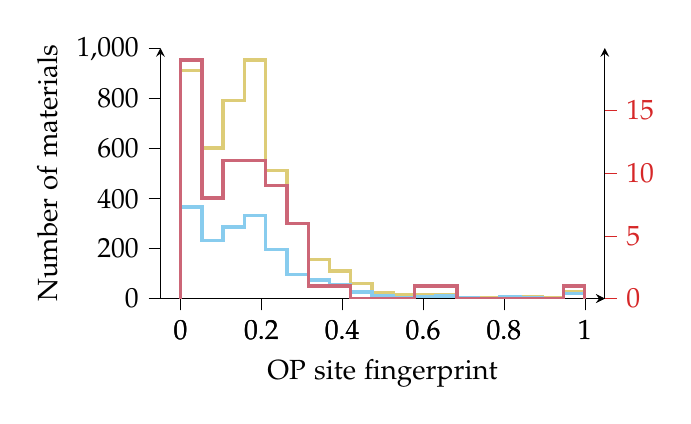
\begin{tikzpicture}

\definecolor{color0}{rgb}{0.866666666666667,0.8,0.466666666666667}
\definecolor{color1}{rgb}{0.533333333333333,0.8,0.933333333333333}
\definecolor{color2}{rgb}{0.83921568627451,0.152941176470588,0.156862745098039}
\definecolor{color3}{rgb}{0.8,0.4,0.466666666666667}

\begin{axis}[
height=1.875590092707901in,
legend cell align={left},
legend style={fill opacity=0.8, draw opacity=1, text opacity=1, draw=white!80!black},
tick align=outside,
tick pos=left,
width=2.8444876158848764in,
x grid style={white!69.0196078431373!black},
xlabel={OP site fingerprint},
xmin=-0.04945, xmax=1.04945,
xtick style={color=black},
y grid style={white!69.0196078431373!black},
ylabel={Number of materials},
ymin=0, ymax=1002.75,
ytick style={color=black}
]
\path [draw=color0, very thick]
(axis cs:0.0005,0)
--(axis cs:0.0005,913)
--(axis cs:0.0530789473684211,913)
--(axis cs:0.0530789473684211,602)
--(axis cs:0.105657894736842,602)
--(axis cs:0.105657894736842,793)
--(axis cs:0.158236842105263,793)
--(axis cs:0.158236842105263,955)
--(axis cs:0.210815789473684,955)
--(axis cs:0.210815789473684,512)
--(axis cs:0.263394736842105,512)
--(axis cs:0.263394736842105,301)
--(axis cs:0.315973684210526,301)
--(axis cs:0.315973684210526,156)
--(axis cs:0.368552631578947,156)
--(axis cs:0.368552631578947,110)
--(axis cs:0.421131578947369,110)
--(axis cs:0.421131578947369,61)
--(axis cs:0.47371052631579,61)
--(axis cs:0.47371052631579,24)
--(axis cs:0.526289473684211,24)
--(axis cs:0.526289473684211,16)
--(axis cs:0.578868421052632,16)
--(axis cs:0.578868421052632,17)
--(axis cs:0.631447368421053,17)
--(axis cs:0.631447368421053,15)
--(axis cs:0.684026315789474,15)
--(axis cs:0.684026315789474,4)
--(axis cs:0.736605263157895,4)
--(axis cs:0.736605263157895,5)
--(axis cs:0.789184210526316,5)
--(axis cs:0.789184210526316,4)
--(axis cs:0.841763157894737,4)
--(axis cs:0.841763157894737,6)
--(axis cs:0.894342105263158,6)
--(axis cs:0.894342105263158,5)
--(axis cs:0.946921052631579,5)
--(axis cs:0.946921052631579,26)
--(axis cs:0.9995,26)
--(axis cs:0.9995,0);

\path [draw=color1, very thick]
(axis cs:0.0005,0)
--(axis cs:0.0005,366)
--(axis cs:0.0530789473684211,366)
--(axis cs:0.0530789473684211,232)
--(axis cs:0.105657894736842,232)
--(axis cs:0.105657894736842,287)
--(axis cs:0.158236842105263,287)
--(axis cs:0.158236842105263,332)
--(axis cs:0.210815789473684,332)
--(axis cs:0.210815789473684,197)
--(axis cs:0.263394736842105,197)
--(axis cs:0.263394736842105,96)
--(axis cs:0.315973684210526,96)
--(axis cs:0.315973684210526,75)
--(axis cs:0.368552631578947,75)
--(axis cs:0.368552631578947,55)
--(axis cs:0.421131578947369,55)
--(axis cs:0.421131578947369,26)
--(axis cs:0.47371052631579,26)
--(axis cs:0.47371052631579,10)
--(axis cs:0.526289473684211,10)
--(axis cs:0.526289473684211,4)
--(axis cs:0.578868421052632,4)
--(axis cs:0.578868421052632,8)
--(axis cs:0.631447368421053,8)
--(axis cs:0.631447368421053,10)
--(axis cs:0.684026315789474,10)
--(axis cs:0.684026315789474,2)
--(axis cs:0.736605263157895,2)
--(axis cs:0.736605263157895,1)
--(axis cs:0.789184210526316,1)
--(axis cs:0.789184210526316,6)
--(axis cs:0.841763157894737,6)
--(axis cs:0.841763157894737,2)
--(axis cs:0.894342105263158,2)
--(axis cs:0.894342105263158,1)
--(axis cs:0.946921052631579,1)
--(axis cs:0.946921052631579,19)
--(axis cs:0.9995,19)
--(axis cs:0.9995,0);
\end{axis}

\begin{axis}[
axis y line=right,
height=1.875590092707901in,
tick align=outside,
width=2.8444876158848764in,
x grid style={white!69.0196078431373!black},
xmin=-0.04945, xmax=1.04945,
xtick pos=left,
xtick style={color=black},
y grid style={white!69.0196078431373!black},
ymin=0, ymax=19.95,
ytick pos=right,
ytick style={color=color2},
yticklabel style={anchor=west, color=color2}
]
\path [draw=color3, very thick]
(axis cs:0.0005,0)
--(axis cs:0.0005,19)
--(axis cs:0.0530789473684211,19)
--(axis cs:0.0530789473684211,8)
--(axis cs:0.105657894736842,8)
--(axis cs:0.105657894736842,11)
--(axis cs:0.158236842105263,11)
--(axis cs:0.158236842105263,11)
--(axis cs:0.210815789473684,11)
--(axis cs:0.210815789473684,9)
--(axis cs:0.263394736842105,9)
--(axis cs:0.263394736842105,6)
--(axis cs:0.315973684210526,6)
--(axis cs:0.315973684210526,1)
--(axis cs:0.368552631578947,1)
--(axis cs:0.368552631578947,1)
--(axis cs:0.421131578947369,1)
--(axis cs:0.421131578947369,0)
--(axis cs:0.47371052631579,0)
--(axis cs:0.47371052631579,0)
--(axis cs:0.526289473684211,0)
--(axis cs:0.526289473684211,0)
--(axis cs:0.578868421052632,0)
--(axis cs:0.578868421052632,1)
--(axis cs:0.631447368421053,1)
--(axis cs:0.631447368421053,1)
--(axis cs:0.684026315789474,1)
--(axis cs:0.684026315789474,0)
--(axis cs:0.736605263157895,0)
--(axis cs:0.736605263157895,0)
--(axis cs:0.789184210526316,0)
--(axis cs:0.789184210526316,0)
--(axis cs:0.841763157894737,0)
--(axis cs:0.841763157894737,0)
--(axis cs:0.894342105263158,0)
--(axis cs:0.894342105263158,0)
--(axis cs:0.946921052631579,0)
--(axis cs:0.946921052631579,1)
--(axis cs:0.9995,1)
--(axis cs:0.9995,0);
\end{axis}

\end{tikzpicture}
}
    \subcaption{}
\end{subfigure}
\begin{subfigure}[b]{0.45\textwidth}
    \scalebox{0.85}{% This file was created with tikzplotlib v0.9.16.
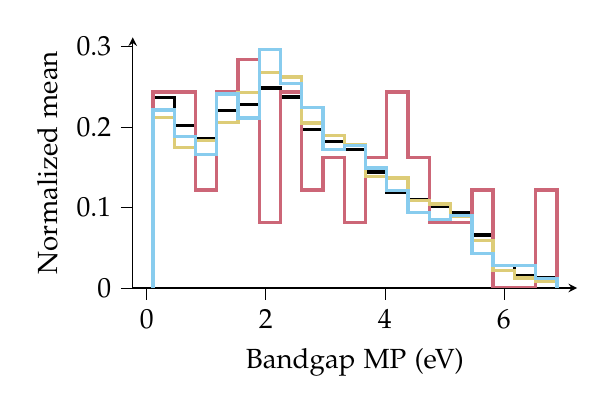
\begin{tikzpicture}

\definecolor{color0}{rgb}{0.8,0.4,0.466666666666667}
\definecolor{color1}{rgb}{0.866666666666667,0.8,0.466666666666667}
\definecolor{color2}{rgb}{0.533333333333333,0.8,0.933333333333333}

\begin{axis}[
height=1.875590092707901in,
legend cell align={left},
legend style={fill opacity=0.8, draw opacity=1, text opacity=1, draw=white!80!black},
tick align=outside,
tick pos=left,
width=2.8444876158848764in,
x grid style={white!69.0196078431373!black},
xlabel={Bandgap MP (eV)},
xmin=-0.234255, xmax=7.229355,
xtick style={color=black},
y grid style={white!69.0196078431373!black},
ylabel={Normalized mean},
ymin=0, ymax=0.311403263332343,
ytick style={color=black}
]
\path [draw=black, very thick]
(axis cs:0.105,0)
--(axis cs:0.105,0.236513148142053)
--(axis cs:0.462110526315789,0.236513148142053)
--(axis cs:0.462110526315789,0.201717735548859)
--(axis cs:0.819221052631579,0.201717735548859)
--(axis cs:0.819221052631579,0.185455961965786)
--(axis cs:1.17633157894737,0.185455961965786)
--(axis cs:1.17633157894737,0.22025137455898)
--(axis cs:1.53344210526316,0.22025137455898)
--(axis cs:1.53344210526316,0.227784402027609)
--(axis cs:1.89055263157895,0.227784402027609)
--(axis cs:1.89055263157895,0.248350762735614)
--(axis cs:2.24766315789474,0.248350762735614)
--(axis cs:2.24766315789474,0.237350151194123)
--(axis cs:2.60477368421053,0.237350151194123)
--(axis cs:2.60477368421053,0.196695717236439)
--(axis cs:2.96188421052632,0.196695717236439)
--(axis cs:2.96188421052632,0.18162966229918)
--(axis cs:3.31899473684211,0.18162966229918)
--(axis cs:3.31899473684211,0.17230305686183)
--(axis cs:3.67610526315789,0.17230305686183)
--(axis cs:3.67610526315789,0.143964524956032)
--(axis cs:4.03321578947368,0.143964524956032)
--(axis cs:4.03321578947368,0.118854433393934)
--(axis cs:4.39032631578947,0.118854433393934)
--(axis cs:4.39032631578947,0.110364831008653)
--(axis cs:4.74743684210526,0.110364831008653)
--(axis cs:4.74743684210526,0.101516513029628)
--(axis cs:5.10454736842105,0.101516513029628)
--(axis cs:5.10454736842105,0.0941030574255792)
--(axis cs:5.46165789473684,0.0941030574255792)
--(axis cs:5.46165789473684,0.066003669248945)
--(axis cs:5.81876842105263,0.066003669248945)
--(axis cs:5.81876842105263,0.0282189600412156)
--(axis cs:6.17587894736842,0.0282189600412156)
--(axis cs:6.17587894736842,0.0159030579893291)
--(axis cs:6.53298947368421,0.0159030579893291)
--(axis cs:6.53298947368421,0.0132724769685379)
--(axis cs:6.8901,0.0132724769685379)
--(axis cs:6.8901,0);

\path [draw=color0, very thick]
(axis cs:0.105,0)
--(axis cs:0.105,0.243500304054985)
--(axis cs:0.462110526315789,0.243500304054985)
--(axis cs:0.462110526315789,0.243500304054985)
--(axis cs:0.819221052631579,0.243500304054985)
--(axis cs:0.819221052631579,0.121750152027492)
--(axis cs:1.17633157894737,0.121750152027492)
--(axis cs:1.17633157894737,0.243500304054985)
--(axis cs:1.53344210526316,0.243500304054985)
--(axis cs:1.53344210526316,0.284083688064149)
--(axis cs:1.89055263157895,0.284083688064149)
--(axis cs:1.89055263157895,0.0811667680183283)
--(axis cs:2.24766315789474,0.0811667680183283)
--(axis cs:2.24766315789474,0.243500304054985)
--(axis cs:2.60477368421053,0.243500304054985)
--(axis cs:2.60477368421053,0.121750152027492)
--(axis cs:2.96188421052632,0.121750152027492)
--(axis cs:2.96188421052632,0.162333536036657)
--(axis cs:3.31899473684211,0.162333536036657)
--(axis cs:3.31899473684211,0.0811667680183284)
--(axis cs:3.67610526315789,0.0811667680183284)
--(axis cs:3.67610526315789,0.162333536036656)
--(axis cs:4.03321578947368,0.162333536036656)
--(axis cs:4.03321578947368,0.243500304054985)
--(axis cs:4.39032631578947,0.243500304054985)
--(axis cs:4.39032631578947,0.162333536036657)
--(axis cs:4.74743684210526,0.162333536036657)
--(axis cs:4.74743684210526,0.0811667680183287)
--(axis cs:5.10454736842105,0.0811667680183287)
--(axis cs:5.10454736842105,0.0811667680183283)
--(axis cs:5.46165789473684,0.0811667680183283)
--(axis cs:5.46165789473684,0.121750152027492)
--(axis cs:5.81876842105263,0.121750152027492)
--(axis cs:5.81876842105263,0)
--(axis cs:6.17587894736842,0)
--(axis cs:6.17587894736842,0)
--(axis cs:6.53298947368421,0)
--(axis cs:6.53298947368421,0.121750152027492)
--(axis cs:6.8901,0.121750152027492)
--(axis cs:6.8901,0);

\path [draw=color1, very thick]
(axis cs:0.105,0)
--(axis cs:0.105,0.211705159535762)
--(axis cs:0.462110526315789,0.211705159535762)
--(axis cs:0.462110526315789,0.1748597187906)
--(axis cs:0.819221052631579,0.1748597187906)
--(axis cs:0.819221052631579,0.18297820573445)
--(axis cs:1.17633157894737,0.18297820573445)
--(axis cs:1.17633157894737,0.205460169578955)
--(axis cs:1.53344210526316,0.205460169578955)
--(axis cs:1.53344210526316,0.242930109319798)
--(axis cs:1.89055263157895,0.242930109319798)
--(axis cs:1.89055263157895,0.267910069147027)
--(axis cs:2.24766315789474,0.267910069147027)
--(axis cs:2.24766315789474,0.262289578185901)
--(axis cs:2.60477368421053,0.262289578185901)
--(axis cs:2.60477368421053,0.204835670583274)
--(axis cs:2.96188421052632,0.204835670583274)
--(axis cs:2.96188421052632,0.189223195691257)
--(axis cs:3.31899473684211,0.189223195691257)
--(axis cs:3.31899473684211,0.178606712764685)
--(axis cs:3.67610526315789,0.178606712764685)
--(axis cs:3.67610526315789,0.138638777041119)
--(axis cs:4.03321578947368,0.138638777041119)
--(axis cs:4.03321578947368,0.136765280054077)
--(axis cs:4.39032631578947,0.136765280054077)
--(axis cs:4.39032631578947,0.108662825248444)
--(axis cs:4.74743684210526,0.108662825248444)
--(axis cs:4.74743684210526,0.10429133227868)
--(axis cs:5.10454736842105,0.10429133227868)
--(axis cs:5.10454736842105,0.0893033563823422)
--(axis cs:5.46165789473684,0.0893033563823422)
--(axis cs:5.46165789473684,0.0593274045896679)
--(axis cs:5.81876842105263,0.0593274045896679)
--(axis cs:5.81876842105263,0.021857464848825)
--(axis cs:6.17587894736842,0.021857464848825)
--(axis cs:6.17587894736842,0.0124899799136143)
--(axis cs:6.53298947368421,0.0124899799136143)
--(axis cs:6.53298947368421,0.00811848694384929)
--(axis cs:6.8901,0.00811848694384929)
--(axis cs:6.8901,0);
\path [draw=color2, very thick]
(axis cs:0.105,0)
--(axis cs:0.105,0.221202002367094)
--(axis cs:0.462110526315789,0.221202002367094)
--(axis cs:0.462110526315789,0.188431335349747)
--(axis cs:0.819221052631579,0.188431335349747)
--(axis cs:0.819221052631579,0.165491868437604)
--(axis cs:1.17633157894737,0.165491868437604)
--(axis cs:1.17633157894737,0.240864402577503)
--(axis cs:1.53344210526316,0.240864402577503)
--(axis cs:1.53344210526316,0.21137080226189)
--(axis cs:1.89055263157895,0.21137080226189)
--(axis cs:1.89055263157895,0.296574536506993)
--(axis cs:2.24766315789474,0.296574536506993)
--(axis cs:2.24766315789474,0.253972669384442)
--(axis cs:2.60477368421053,0.253972669384442)
--(axis cs:2.60477368421053,0.224479069068829)
--(axis cs:2.96188421052632,0.224479069068829)
--(axis cs:2.96188421052632,0.172046001841073)
--(axis cs:3.31899473684211,0.172046001841073)
--(axis cs:3.31899473684211,0.176961601893676)
--(axis cs:3.67610526315789,0.176961601893676)
--(axis cs:3.67610526315789,0.14910653492893)
--(axis cs:4.03321578947368,0.14910653492893)
--(axis cs:4.03321578947368,0.121251467964185)
--(axis cs:4.39032631578947,0.121251467964185)
--(axis cs:4.39032631578947,0.0933964009994398)
--(axis cs:4.74743684210526,0.0933964009994398)
--(axis cs:4.74743684210526,0.0852037342451034)
--(axis cs:5.10454736842105,0.0852037342451034)
--(axis cs:5.10454736842105,0.090119334297705)
--(axis cs:5.46165789473684,0.090119334297705)
--(axis cs:5.46165789473684,0.0426018671225515)
--(axis cs:5.81876842105263,0.0426018671225515)
--(axis cs:5.81876842105263,0.0278550669647452)
--(axis cs:6.17587894736842,0.0278550669647452)
--(axis cs:6.17587894736842,0.0278550669647452)
--(axis cs:6.53298947368421,0.0278550669647452)
--(axis cs:6.53298947368421,0.0114697334560715)
--(axis cs:6.8901,0.0114697334560715)
--(axis cs:6.8901,0);

\end{axis}

\end{tikzpicture}
}
    \subcaption{}
\end{subfigure}
\caption{Number of predicted suitable materials as a function of the (a) covalent radius, (b) maximum packing efficiency, and standard deviation of the radial distribution function with center at (c) $2.0$ and (d) $3.0$. Panel (e) shows standard deviation of the chemical environment of the gaussian symmetric function. Panels (f) crystal fingerprint and (g) OP site fingerprint are related to bond orientational parameters, while (h) shows the band gap referenced to the normalized mean of the entire data set. 
%The total number of predicted materials is  $6804$ for the Ferrenti approach, $9227$ for the extended Ferrenti approach, and $214$ for the empirical approach. 
The Ferrenti and extended Ferrenti approaches refer to the left y-axis and the empirical approach to the right. All panels were taken for a $0.75$ cut-off. }
\label{fig:histograms_supp}
\end{figure}


Firstly, we find that the covalent radii of the materials (see Fig.~\ref{fig:histograms_supp}a) distribute with two peaks in the data in all approaches. The maxima are slightly shifted towards the right for the empirical approach compared to the two others but otherwise the data distributions are similar. The trend of two data peaks is repeated for the maximum packing efficiency (see Fig.~\ref{fig:histograms_supp}b) but is much more prominent for the empirical approach. This indicates that the material density, or in other words the bond length, is an important parameter for QT suitability.  

\bibliography{apssamp}% Produces the bibliography via BibTeX.

\end{document}

